%%%%%%%%%%%%%%%%%%%%%%%%%%%%%%%%%%%%%%%%%%%%%%%%%%%%%%%%%%%%%%%%%%%%%%%%%%%%%%%%
% M7M02 (Ammonite) Microcontroller Hypervisor -- Chinese User Manual
%
% Build with XeLaTeX:
%   latexmk -xelatex -outdir=Build rvm-manual.tex
%
% Nine-chapter R3T1 organisation.
%%%%%%%%%%%%%%%%%%%%%%%%%%%%%%%%%%%%%%%%%%%%%%%%%%%%%%%%%%%%%%%%%%%%%%%%%%%%%%%%
\documentclass[10pt,a4paper,twoside,openany]{book}
\usepackage{rvm-style}

\begin{document}

\frontmatter
\begin{titlepage}
    \thispagestyle{empty}
    \centering
    \vspace*{1.6cm}
    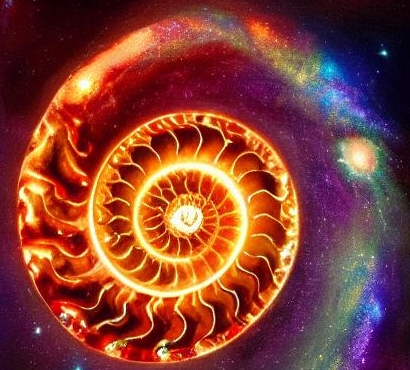
\includegraphics[width=5.55cm]{Figure/logo.png}\par
    \vspace{0.55cm}
    {\sffamily\small\color{rvmmid}AMMONITE\par}
    \vfill
    {\sffamily\fontsize{28}{34}\selectfont\color{rvmpurple}
        M7M02（Ammonite）R3T1\\[6pt]
        微控制器嵌入式虚拟机监视器\\[2pt]
        （三版一型）\par}
    \vspace{1.1em}
    {\sffamily\fontsize{21}{25}\selectfont\color{rvmgray}技术参考手册\par}
    \vspace{1.4em}
    {\rmfamily\large\color{rvmmid}
    版本 R3T1\quad$\cdot$\quad 二〇二五年三月二十日\par}
    \vfill
    {\sffamily\small\color{rvmmid}
    EDI-Systems\quad$\cdot$\quad \texttt{www.edi-systems.org}\par}
    \vspace*{1.4cm}
\end{titlepage}

\chapter*{系统特性}
\addcontentsline{toc}{chapter}{系统特性}
\markboth{系统特性}{}

\begin{center}
{\sffamily\large\color{rvmgray}突越·中生·菊石（七阶）}\\[4pt]
{\sffamily\large\color{rvmgray}Mutatus·Mesozoa·Ammonite（R.VII）}\\[10pt]
{\sffamily\large\color{rvmgray}M7M02（Ammonite）R3T1}\\[4pt]
{\sffamily\Large\bfseries\color{rvmgray}微控制器嵌入式虚拟机监视器（三版一型）}\\[8pt]
{\rmfamily\color{rvmmid}技术手册}\\[12pt]
\end{center}

\begin{description}[leftmargin=0pt,labelindent=0pt,style=nextline,itemsep=8pt]
    \item[\textsf{\color{rvmpurple}高性能实时响应}]
    原生进程提供优秀的实时性能。
    虚拟机进程提供优秀的兼容性和执行效率。

    \item[\textsf{\color{rvmpurple}全面的体系架构支持}]
    可简易地在多种架构之间移植。
    在微控制器上支持准虚拟化。

    \item[\textsf{\color{rvmpurple}高安全性}]
    虚拟机之间硬件隔离。
    支持故障重启功能。

    \item[\textsf{\color{rvmpurple}全面的生态环境}]
    支持虚拟化绝大多数操作系统。
    原系统应用程序无需修改即可使用。

    \item[\textsf{\color{rvmpurple}高易用性}]
    提供带图形化界面的工程生成器。
\end{description}

\newcommand{\RVMRevisionHistory}{%
\chapter*{版本历史}
\addcontentsline{toc}{chapter}{版本历史}
\markboth{版本历史}{}
\begin{table}[htbp]
    \centering
    \renewcommand{\arraystretch}{1.25}
    \small
    \begin{tabularx}{\textwidth}{@{}>{\sffamily\bfseries\color{rvmpurple}}m{1.8cm}
                                  >{\raggedright\arraybackslash}m{3.2cm}X@{}}
    \toprule
    版本 & 日期（年-月-日） & 说明 \\
    \midrule
    R1T1 & 2018-03-09 & 初始发布。 \\
    R2T1 & 2018-09-18 & 增加了移植说明。 \\
    R3T1 & 2025-03-20 & 发布 R3T1 技术参考手册。 \\
    \bottomrule
    \end{tabularx}
\end{table}
}


\tableofcontents
\clearpage
\phantomsection
\addcontentsline{toc}{chapter}{表目录}
\listoftables
\clearpage
\phantomsection
\addcontentsline{toc}{chapter}{图目录}
\listoffigures
\clearpage
\RVMRevisionHistory

\mainmatter
\chapter{概述}\label{ch:1-overview}

\section{简介}\label{sec:1-1}

在现代微控制器（MCU）应用中，人们对灵活性、安全性和可靠性的要求日益提高。越来越多的微控制器应用要求多个互不信任的来源的应用程序一起运行，也可能同时要求实时可靠部分\footnote{如电机控制等}、性能优先部分\footnote{如网络协议栈、高级语言虚拟机等}和某些对信息安全有要求的应用\footnote{如加解密算法等}一起运行，而且互相之间不能干扰。在某些应用程序宕机时，要求它们能够单独重启，并且在此过程中还要求保证那些直接控制物理机电输出的应用程序不受干扰。

由于传统实时操作系统（Real-Time Operating
System，RTOS）的内核和应用程序通常静态链接在一起，而且互相之间没有内存保护隔离，因此达不到应用间信息隔离的要求；一旦其中一个应用程序崩溃而破坏内核数据，其他所有应用程序必然同时崩溃。一部分RTOS号称提供了内存保护，但是其具体实现机理表明其内存保护仅仅能够提供一定程度的应用间可靠性而无法提供应用间安全性，不适合现代微控制器应用的信息安全要求。此外，传统RTOS的内核服务\footnote{如内核定时器等}是在高优先级应用和低优先级应用之间共用的，一旦低优先级应用调用大量的内核服务，势必影响高优先级应用内核服务的响应，从而造成时间干扰问题\protect\hyperref[cite:1-1]{{[}1{]}}。

RVM（Real-time Virtual machine
Monitor）就是针对上述问题而提出的、面向高性能MCU的、基于RME微内核的用户态库。它是运行在RME操作系统上的一个宿主型虚拟机监视器，使得在微控制器平台上运行多个虚拟机成为可能，也同时满足用户运行原生RME应用程序的需求。这样，实时和非实时应用一起运行的需求，在实时应用和非实时应用之间不会产生时间干扰。它也能够使多来源应用程序在同一芯片上运行而不发生信息安全问题。

由于RVM强制隔离了系统中安全的部分和不安全的部分，这两部分就可以用不同的标准分开开发和认证。这方便了调试，也节省了开发和认证成本，尤其是当使用到那些较为复杂、认证程度较低和实时性较差的的软件包如用户图形界面（Graphical
User
Interface，GUI）和高级语言虚拟机（Python、Java虚拟机）等的时候。此外，在老平台上已得到认证的微控制器应用程序可以作为一个虚拟机直接运行在RVM上，无需重新认证；这进一步节省了成本。

本手册从用户的角度提供了RVM的功能描述。关于各个架构的具体使用，请参看各个架构相应的手册。在本手册中，我们先简要回顾关于虚拟化的若干概念，然后分章节介绍RVM的特性和API。

\subsection{微控制器的特点}\label{subsec:1-1-1}

在实际应用中，MCU系统占据了实时系统中的相当部分。它常常有如下几个特点：

\subsubsection{深度嵌入}\label{subsubsec:1-1-1-1}

微控制器的应用场合往往和设备本身融为一体，用户通常无法直接感知到此类系统的存在。微控制器的应用程序\footnote{通常称为``固件''}一旦写入，往往在整个生命周期中不再更改，或者很少更改。即便有升级的需求，往往也由厂家进行升级。

\subsubsection{高度可靠}\label{subsubsec:1-1-1-2}

微控制器应用程序对于可靠性有近乎偏执的追求，任何系统故障都会引起相对严重的后果。从小型电压力锅到大型起重机，这些系统都不允许发生严重错误，否则会造成重大财产损失或人身伤亡。此外，对于应用的实时性也有非常高的要求，它们通常要么要求整个系统都是硬实时系统，或者系统中直接控制物理系统的那部分为硬实时系统。

\subsubsection{资源有限}\label{subsubsec:1-1-1-3}

由于微控制器本身资源不多，因此高效地利用它们就非常重要了。微控制器所使用的软件无论是在编写上和编译上总体都为空间复杂度优化，只有小部分对性能和功能至关重要的程序使用时间复杂度优化。

\subsubsection{静态分配和链接}\label{subsubsec:1-1-1-4}

与微处理器不同，由于深度嵌入的原因，微控制器应用中的绝大部分资源，包括内存和设备在内，都是在系统上电时创建并分配的。通常而言，在微控制器内使用过多的动态特性是不明智的，因为动态特性不仅会对系统的实时响应造成压力，另一方面也会增加功能成功执行的不确定性。如果某些至关重要的功能和某个普通功能都依赖于动态内存分配，那么当普通功能耗尽内存时，可能导致重要功能的内存分配失败。基于同样的或类似的理由，在微控制器中绝大多数代码都是静态链接的，一般不使用动态链接。

\subsubsection{仅物理地址空间}\label{subsubsec:1-1-1-5}

与微处理器不同，微控制器通常都不具备内存管理单元（Memory Management
Unit，MMU），因此无法实现物理地址到虚拟地址的转换。但是，RVM也支持使用内存保护单元（Memory
Protection
Unit，MPU），并且大量的中高端微控制器都具备MPU。与MMU不同，MPU往往仅支持保护一段或几段内存范围，有些还有很复杂的地址对齐限制，因此内存管理功能在微控制器上往往是有很大局限性的。

\subsubsection{单核处理器}\label{subsubsec:1-1-1-6}

如今，绝大多数的微处理器都是多核设计。然而，与微处理器不同，微控制器通常均为单核设计，因此无需考虑很多竞争冒险问题。这可以进一步简化微控制器用户态库的设计。考虑到的确有少部分微控制器采取多核设计或者甚至不对称多核设计，RVM也支持多核运行环境。当然，这首先需要底层的RME被正确配置为支持多核。

考虑到以上几点，在设计RVM时，所有的内核对象都会在系统启动时创建完全，并且在此时，系统中可用内核对象的上限也就决定了。各个虚拟机则被固化于微控制器的片上非易失性存储器中。

\subsection{软件版权与许可证}\label{subsec:1-1-2}

综合考虑到微控制器应用、深度嵌入式应用和传统应用对开源系统的不同要求，RVM微控制器库所采用的许可证为Unlicensed，但是对一些特殊情况\footnote{比如安防器材、军工系统、航空航天装备、电力系统和医疗器材等}使用特殊的规定。这些特殊规定是就事论事的，对于每一种可能情况的具体条款都会有不同。

\subsection{主要参考系统}\label{subsec:1-1-3}

RTOS通用服务主要参考了如下系统的实现：

\begin{quote}
RMProkaron（@EDI）

FreeRTOS（@Real-Time Engineering LTD）

Contiki（@The Contiki Community）
\end{quote}

\needspace{8\baselineskip}
Contiki虚拟机监视器的设计参考了如下系统的实现：

\begin{quote}
Nova（@TU Dresden）

XEN（@Cambridge University）

KVM（@The Linux Foundation）
\end{quote}

其他各章的参考文献和参考资料在该章列出。

\section{前言}\label{sec:1-2}

作为一个虚拟机监视器，RVM依赖于底层RME操作系统提供的内核服务来维持运行。RVM采用准虚拟化技术，最大限度节省虚拟化开销，典型情况下仅增加约1\%的CPU开销。

RVM完全支持低功耗技术，可以实现虚拟化系统的各个分区处于无节拍工作，最大限度减少电力需求。

对于RME原生进程应用，其响应时间和FreeRTOS一档小型RTOS的响应时间相若，完全能够满足那些对实时性要求最苛刻的应用。

对于RVM宿主型虚拟机\footnote{虚拟机分类见下文所述}，中断响应时间和线程切换时间将会增加到原小型RTOS的约4倍。值得注意的是，RVM本身并不提供任何POSIX支持；POSIX支持是依赖于所移植的操作系统本身的。幸运的是，很多RTOS都具备POSIX支持，因此直接虚拟化它们就可以使用其POSIX功能了。

RME和RVM在全功能配置下共占用最小16kB内存\footnote{此时可支持4个虚拟机，若分配128kB内存则可支持32个虚拟机}，外加固定占用48kB程序存储器，适合中高性能微控制器使用。此外，如果多个RVM虚拟机同时使用网络协议栈等组件，使用本技术甚至可节省内存，因为网络协议栈等共享组件可以只在系统中创建一个副本，而且多个操作系统的底层切换代码和管理逻辑由于完全被抽象出去，因此在系统中只有一个副本。

在此我们回顾一下虚拟化的种类。在本手册中，我们把虚拟机按照其运行平台分成三类，分别称为原生型（I型）、宿主型（II型）和容器型（III型）。同时，依照虚拟机支持虚拟化方式的不同，又可以分为全虚拟化型（Full
Virtualization，FV）和准虚拟化型（Para-Virtualization，PV）。这两种分类方法是互相独立的。

\subsection{原生型虚拟机监视器}\label{subsec:1-2-1}

原生型虚拟机监视器作为底层软件直接运行在硬件上，创造出多个物理机的实例，也叫I型虚拟机监视器。多个虚拟机在这些物理机的实例上运行。这类虚拟机监视器的优势在于高性能、低开销，但缺点则是自身不具备虚拟机管理功能，需要0域\footnote{也即第一个启动的、具有管理特权的虚拟机}对其他虚拟机进行管理，且无法像常规操作系统那样运行轻量级的普通进程。此类虚拟机监视器有KVM\footnote{KVM模糊了原生型和宿主型的边界，严格地讲不属于其中任何一类}、Hyper-V、VMware ESXi Server、Xen、XtratuM等。

\subsection{宿主型虚拟机监视器}\label{subsec:1-2-2}

宿主型虚拟机监视器作为应用程序运行在操作系统上，创造出多个物理机的实例，也叫II型虚拟机监视器。多个虚拟机在这些物理机的实例上运行。这类虚拟机的优势在于系统独立、自身具备一定的管理功能，并允许将它们的虚拟机进程和其它普通的宿主机进程一起调度，因此得到了最广泛的应用，但效率通常认为比原生型要低一些。此类虚拟机监视器有VMware Workstation、Virtual Box、QEMU\footnote{不包括其KVM版本}等。RVM是在RME上开发的一个应用程序，其虚拟机也作为进程运行在RME上，因此也属于宿主型虚拟机监视器。

\subsection{容器型虚拟机监视器}\label{subsec:1-2-3}

容器型虚拟机监视器是由操作系统本身提供的功能，创造出多个相互隔离的操作系统资源分配空间的独立实例，严格来讲并不属于虚拟机监视器，但由于它也具有一定的资源分区功能而在某些场合被称为III型虚拟机监视器。多个应用程序直接在这些资源分配空间实例上运行。通常而言，这类虚拟机监视器的性能最高，虚拟化的内存和时间开销最低，但是它要求应用程序必须是针对它提供的接口编写的。通常而言，这接口与操作系统自身的系统调用一致，而其它接口均不被兼容，因而普适性很差。此类虚拟机监视器有Docker、Pouch、RKT、LXC等。当RVM导致的性能开销被认为不合适时，由于RME操作系统自身也原生具备容器型虚拟机监视器的能力，也可以不使用RVM而把其提供的用户态库用来开发原生的容器型虚拟机应用。事实上，如果不在RVM配置文件中声明任何虚拟机，RVM的虚拟化功能会在编译时被从系统中自动去掉以适应资源极端的环境\footnote{如Cortex-M0+等RAM在20KiB上下的环境}。

\subsection{全虚拟化型虚拟机监视器}\label{subsec:1-2-4}

全虚拟化型虚拟机监视器是有能力创建和原裸机完全一致的硬件实例的虚拟机监视器。通常而言，这需要MMU的介入来进行地址转换，而且对特权指令要进行二进制翻译、陷阱重定向或专用硬件\footnote{如Intel VT-x、AMD AMD-V等}处理，对于I/O也需要特殊硬件功能\footnote{如Intel VT-d等}来重定向。此类虚拟机在MCU环境上难于实现，因为微控制器通常都不提供MMU，也不提供相应的虚拟化硬件进行重定向功能。此类虚拟机监视器有VMware Workstation、Virtual Box、QEMU、KVM、Hyper-V、ESX Server等。

\subsection{准虚拟化型虚拟机监视器}\label{subsec:1-2-5}

准虚拟化型虚拟机监视器是创建了和原裸机有些许差别的硬件实例的虚拟机监视器。它使用超调用（Hypercall）处理特权指令和特殊I/O，并借此避开那些复杂、不必要的全虚拟化必须提供的细节。此类虚拟机在MCU环境上能够以较高的性能实现。此类虚拟机监视器有Xen等。RVM也是一个准虚拟化型虚拟机监视器，通过超调用处理系统功能。

\section{手册总览}\label{sec:1-3}

本手册从用户的角度解释了RVM的基本组成与运行原理，并假定读者对虚拟化的基本概念有一般了解。在本手册中，所有的typedef类型之前的``rvm\_''前缀均被省去。

本手册的第一部分为\protect\hyperref[sec:2-1]{第2章}
。在该章节中将概略描述RVM的架构，推荐详细阅读。

本手册的第二部分为第3章到第5章。在这些章节中将分别详细描述RVM的技术细节，推荐按需查阅。其中，\protect\hyperref[sec:3-1]{第3章}
介绍原生进程的细节信息，\protect\hyperref[sec:4-1]{第4章}
介绍虚拟机的细节信息，\protect\hyperref[sec:5-1]{第5章}
介绍工程生成器的细节信息。

本手册的第三部分为\protect\hyperref[ch:6-using-rvm]{第6章}
。在该章节中将从用户角度详述RVM及其工程生成器的使用方式，推荐详细阅读。

本手册的最后部分为\protect\hyperref[sec:8-1]{第8章}
。在该章节中将详细描述如何移植RVM到新架构。如果用户不需要进行移植，无需阅读该章节。

\needspace{12\baselineskip}
\section{本章参考文献}\label{sec:1-4}

\begin{enumerate}
\def\labelenumi{{[}\arabic{enumi}{]}}
\item
  \protect\phantomsection\label{cite:1-1}
  P. Patel, M. Vanga, and B. B. Brandenburg, ``TimerShield: protecting
  high-priority tasks from low-priority timer interference,'' in
  \textit{Proceedings of the IEEE Real-Time and Embedded Technology and
  Applications Symposium (RTAS)}, 2017, pp. 3--12.
\item
  \protect\phantomsection\label{cite:1-2}
  A. Dunkels, B. Gronvall, and T. Voigt, ``Contiki---a lightweight and
  flexible operating system for tiny networked sensors,'' in
  \textit{Proceedings of the 29th Annual IEEE International Conference
  on Local Computer Networks}, 2004, pp. 455--462.
\end{enumerate}


\chapter{虚拟化架构}\label{ch:2-virtualization-architecture}

\section{架构总览}\label{sec:2-1}

RVM是专为资源受限的微控制器打造的虚拟机监视器，它能够将一颗微控制器分解成时空上互不影响的多颗虚拟微控制器。即便其中一颗虚拟微控制器发生了致命故障，其它虚拟微控制器仍然能保持正常运作，不会受到不利影响，从而有效阻止故障或安全漏洞在整个系统中的扩散。

与常见的KVM、Virtual
Box、VMWare等产品不同，RVM将微控制器的资源静态分配给各颗虚拟微控制器，其资源分配信息在系统编译时就能够确定。三个重要因素导致了这种设计：（1）绝大多数微控制器依赖于Flash存储器保存程序，缺乏加载动态运行时库的能力，（2）微控制器的资源非常少，需要极为高效地进行利用，因此很难承担动态数据结构带来的额外开销，以及（3）在关键系统中引入过多动态性可能导致系统行为难以预测。当然，在各个虚拟微控制器内部，还是可以使用动态内存分配、动态线程创建等功能的；即便这些动态行为导致虚拟微控制器故障，也不会引起其它虚拟微控制器的正常运作。

RVM与传统虚拟化解决方案的另一个不同在于其客户机运行实时操作系统（Real-Time
Operating
System，RTOS）。这些操作系统有两个特点：（1）它们要求系统时延是确定性的，（2）它们要求虚拟化的开销要非常低。常规的虚拟化解决方案往往是基于操作\footnote{或二进制}翻译的，其底层原语往往离客户机操作系统的接口语义有一定偏离，一个简单的客户机请求就有可能被翻译成大量的超级调用（Hypercall），引起上百倍的时延放大。为了解决这个问题，RVM（1）内部的一切代码均是按照实时系统的标准设计的，其执行时延确定，（2）内部操作原语和超级调用的语义上被设计为RTOS友好的，一个RTOS操作仅会被翻译成一个操作原语或超级调用。

RVM与传统虚拟化解决方案的最后不同在于其往往要面临（极端）苛刻的存储器要求。这些要求是相当极端\footnote{某些场合几十个甚至几个字节都要争取}的，但并非不可理解：任何被用于资源隔离的CPU和存储器开销在那些不重视产品质量的设计中都可以节省；偏偏微控制器的价格非常低、用量非常高，任何一点增加的成本都能极大地反映在产品最终的售价上；如果隔离开销过高以至于需要哪怕稍贵一点的微控制器，就得不偿失了。为此，RVM被设计为极端节约存储器。它自身只需要最少5kB
RAM和20kB
ROM即可运行，因而可能是世界上最小的虚拟化环境。这使得它可以普遍用于那些128kB
ROM、64kB RAM的主流微控制器系列，只要它们具备内存保护单元（Memory
Protection Unit，MPU）。

为了应对上述挑战，RVM要求在系统编译时静态确定大量的地址信息，并创建一系列具备特定参数的内核对象。相应的数据结构也是特化设计的，这使得手工填充它们十分困难。为此，RVM还提供了工程生成器，可以根据对系统的描述生成工程所需的初始化代码、链接器脚本甚至是对应于相应构建环境的工程文件。

这样，RME微内核、RVM监视器、运行在其上的原生进程和各RTOS虚拟机，以及用以生成整个工程的工程生成器构成了RME的微控制器操作系统生态。虚拟化的总架构见下图所示：图中实线代表硬件隔离机制，虚线代表软件模组的边界。


\begin{figure}[htbp]
\centering
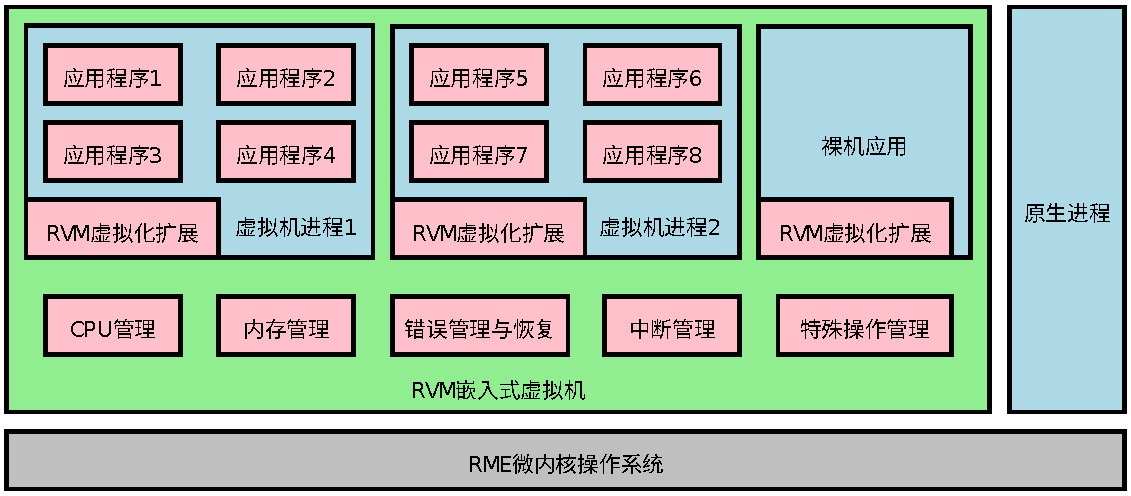
\includegraphics[width=0.90\textwidth]{Figure/image2.pdf}
\caption{RVM架构简图}\label{fig:2-1}
\end{figure}


RVM虚拟机运行在一个基于准虚拟化技术实现的虚拟机监视器上。它实现了虚拟化的所有基本功能：内存管理、CPU管理、中断向量虚拟化和虚拟机错误处理。关于这些实现的具体信息请参见下文所述。

\subsection{RME微内核}\label{subsec:2-1-1}

RME微内核作为RVM的底层支撑存在，负责向RVM提供基本的操作系统服务。其它一切运行在微控制器上的组件都是作为RME进程存在的。有关RME微内核，请参见相关内核文档。

\subsection{RVM虚拟机监视器}\label{subsec:2-1-2}

RVM虚拟机监视器负责具体的虚拟机管理工作，它作为II型虚拟机监视器运行在RME上。具体地，它将物理中断和事件源信号下发到各个虚拟机，并响应来自各个虚拟机的超级调用请求。在虚拟机遇到异常时，RVM还负责重启对应的虚拟机。虚拟机监视器包括五个守护线程：启动守护线程（Initialization
Daemon，INIT）、安全守护协程（Safety Daemon，SFTD）、时间守护协程（Timer
Daemon，TIMD）、向量守护协程（Vector
Daemon，VCTD）和超级调用守护线程（Hypercall
Daemon，HYPD），其中后三个协程，它们共同运行于虚拟化守护线程（Virtual
Machine Monitor Daemon，VMMD）之上。下文将对这五个守护线程加以一一介绍。

\subsubsection{启动守护线程INIT}\label{subsubsec:2-1-2-1}

INIT是RME在启动时创建的，由它负责初始化系统中的原生线程与虚拟机，并启动剩下的四个守护线程。在这一工作完成后，INIT即进入休眠，并仅在系统中无可运行的线程时被调度。它一旦被调度，就反复执行处理器休眠命令，令处理器进入低功耗状态以等待中断来临。

\subsubsection{安全守护协程SFTD}\label{subsubsec:2-1-2-2}

SFTD运行在系统的最高优先级\footnote{Kern\_Prio-1}，负责监控原生进程和虚拟机的运行。它平时阻塞在错误处理端点RVM\_Sftd\_Sig\_Cap上，一旦原生进程和虚拟机发生任何异常，SFTD便解除阻塞开始运行。若发生异常的是原生进程，SFTD将重启整个系统；若发生异常的是虚拟机，则SFTD仅重启该虚拟机。

\subsubsection{向量守护协程VCTD}\label{subsubsec:2-1-2-3}

VCTD运行在较原生进程低，但较虚拟机高的优先级上，负责将系统中的物理中断和事件激活转送给各个虚拟机的中断源。它平时阻塞在中断向量端点RVM\_BOOT\_INIT\_VCT上，一旦该端点收到任何信号，VCTD便解除阻塞开始运行。VCTD将从分别位于RVM\_PHYS\_VCT\_BASE和RVM\_VIRT\_EVT\_BASE的两个RVM\_Flag数据结构中提取中断向量和事件源激活信息，并将其转送给虚拟机。

每个RVM\_Flag数据结构都由两个相同的struct
\_\_RME\_RVM\_Flag合并而成。这是因为，VCTD访问struct
\_\_RME\_RVM\_Flag时需要独占它，而此时内核若需要传递激活信息给RVM，只能选择填充另一个结构体副本。每个结构体内部都有如下三个域：

\begin{xltabular}{\textwidth}{@{}>{\hsize=0.4500\hsize\raggedright\arraybackslash}X>{\hsize=1.5500\hsize\raggedright\arraybackslash}X@{}}
\caption{struct \_\allowbreak{}\_\allowbreak{}RME\_\allowbreak{}RVM\_\allowbreak{}Flag中各个域的意义}\label{tab:2-1}\\
\toprule
域名称 & 作用\tabularnewline
\endfirsthead
\toprule
域名称 & 作用\tabularnewline
\midrule
\endhead
\bottomrule
\endlastfoot
ptr\_\allowbreak{}t Lock &
决定此结构体是否正被VCTD使用。如果VCTD正在使用该结构体，内核无法对此结构体进行操作，否则可能引起竞争冒险。则内核会选择去填充另一个结构体。\tabularnewline
ptr\_\allowbreak{}t Fast &
指示快速信号源的激活。如果为1，则快速中断源激活。当前，这一个域仅在位于RVM\_\allowbreak{}PHYS\_\allowbreak{}VCT\_\allowbreak{}BASE的结构体中使用，用来传达时钟中断信号。\tabularnewline
ptr\_\allowbreak{}t Group &
指示被激活的慢速信号源的组别，是一个位图。若某位被置位，则意味着Flag域中该组别有被激活的信号：如果第2位被置位，则意味着Flag{[}2{]}的某一位不为0。设置该域的目的是快速查找被激活的信号所在的组别。\tabularnewline
ptr\_\allowbreak{}t Flag{[}{]} &
一个位图，指示具体的被激活的信号源。其长度由信号的数量决定：如果某处理器的字长为32位，而有96个中断源，则此域的长度为96/32=3个机器字长。\tabularnewline
\end{xltabular}

比如，在32位处理器上，若34号物理中断源被激活，内核会首先查找位于RVM\_PHYS\_VCT\_BASE的两个struct
\_\_RME\_RVM\_Flag结构体，并选择一个Lock域为0的副本。然后，内核会将Flag{[}1{]}的第{[}2{]}个位置位，并将Group的第{[}1{]}个位置位。最后，内核会向RVM\_BOOT\_INIT\_VCT发送信号，激活VCTD。VCTD被激活后，会交替查找两个struct
\_\_RME\_RVM\_Flag中存在的置位的位。它在查找时，首先将第一个struct
\_\_RME\_RVM\_Flag的Lock置1，然后查询Group中哪些位被置位，并根据该信息查询对应的Flag{[}{]}，得到具体的中断源编号。若激活的是34号中断源，则应当查询到Group的位{[}1{]}置位，并转去查询Flag{[}1{]}；在Flag{[}1{]}中则发现其位{[}2{]}置位。由此，VCTD可以推算出被激活的中断源是第34号，并将登记了34号物理中断源的那些虚拟机激活。有关虚拟机的激活，请参见\protect\hyperref[subsec:2-2-4]{2.2.4}
。

事件源的激活过程与物理中断源的激活过程是类似的。关于事件源，请参见\protect\hyperref[subsec:2-2-7]{2.2.7}
。

\subsubsection{时间守护协程TIMD}\label{subsubsec:2-1-2-4}

时间守护线程TIMD运行在与VCTD相同的优先级上，负责将RVM时钟嘀嗒传递给各个虚拟机。它平时阻塞在时钟中断端点RVM\_BOOT\_INIT\_VCT上，一旦该端点收到定时器中断就将该中断传递给所有虚拟机。TIMD每在时钟中断端点RVM\_BOOT\_INIT\_VCT上收到一次信号，就称作一个RVM时钟嘀嗒。每个虚拟机可以指定一个分频系数Period\footnote{请参见\protect4.2}，在收到Period个RVM时钟嘀嗒后才会向虚拟机发送一个虚拟时钟中断。

时间守护线程还允许为每个虚拟机指定一个看门狗超时时间Watchdog\footnote{请参见\protect4.2}。虚拟机可以使用超级调用RVM\_Hyp\_Wdg\_Clr来投喂看门狗；如果该虚拟机在Watchdog个时钟嘀嗒后仍未喂狗，则判断该虚拟机陷入死循环，此时TIMD将重启它。

\subsubsection{超级调用守护协程HYPD}\label{subsubsec:2-1-2-5}

超级调用守护线程HYPD运行在与VCTD相同的优先级上，负责接受并处理各个虚拟机发来的超级调用。它平时阻塞在超级调用处理端点RVM\_BOOT\_INIT\_VCT上，一旦该端点收到信号就处理当前虚拟机发起的超级调用。有关超级调用的具体处理方法，请参见\protect\hyperref[subsec:2-2-6]{2.2.6}
。

\needspace{14\baselineskip}
\subsection{保护域}\label{subsec:2-1-3}

\needspace{10\baselineskip}
RVM提供两种保护域，分别是原生进程和虚拟机。两者的简要对比如下：

\begin{xltabular}{\textwidth}{@{}>{\hsize=1.0000\hsize\raggedright\arraybackslash}X>{\hsize=1.0000\hsize\raggedright\arraybackslash}X>{\hsize=1.0000\hsize\raggedright\arraybackslash}X>{\hsize=1.0000\hsize\raggedright\arraybackslash}X>{\hsize=1.0000\hsize\raggedright\arraybackslash}X>{\hsize=1.0000\hsize\raggedright\arraybackslash}X>{\hsize=1.0000\hsize\raggedright\arraybackslash}X>{\hsize=1.0000\hsize\raggedright\arraybackslash}X>{\hsize=1.0000\hsize\raggedright\arraybackslash}X@{}}
\caption{原生进程与虚拟机的对比}\label{tab:2-2}\\
\toprule
保护域 & 秘密性 & 完整性 & 可用性 & 可审计性 & 实时性 & 紧凑性 & 可靠性
& 易用性\tabularnewline
\endfirsthead
\toprule
保护域 & 秘密性 & 完整性 & 可用性 & 可审计性 & 实时性 & 紧凑性 & 可靠性
& 易用性\tabularnewline
\midrule
\endhead
\bottomrule
\endlastfoot
原生进程 & 强 & 弱 & 弱 & 弱 & 强 & 强 & 弱 & 弱\tabularnewline
虚拟机 & 强 & 强 & 强 & 强 & 弱 & 弱 & 强 & 强\tabularnewline
\end{xltabular}

\subsubsection{原生进程}\label{subsubsec:2-1-3-1}

RME原生进程直接运行在RME微内核上，它们不受RVM虚拟机监视器的制约，且资源消耗要比虚拟机低。它们主要用来接受从中断向量来的信号，并在进行初步处理后将这些信号转发给虚拟机。原生进程内的线程的时间片都是无限的，且在整个系统中拥有最高的优先级。即使RVM和它负责管理的所有虚拟机都已崩溃，原生进程内的线程仍能正常运行，从而维护被控设备的安全。

即便原生进程不是虚拟机，工程生成器仍对它们提供了完善的支持，RVM的用户态库也提供一系列对系统调用的封装以方便在C程序中使用系统调用。工程生成器甚至可以生成不含虚拟机的工程，此时只能使用原生进程和系统调用来完成应用程序的功能。

RVM没有为原生进程提供容错功能；如果任何一个原生进程发生异常，则RVM的SFTD将认为系统中出现了严重的问题，并重启整个系统。因此，原生进程仅具备安全三要素中的秘密性，一旦被入侵，则系统的完整性和可用性将荡然无存。

\subsubsection{虚拟机}\label{subsubsec:2-1-3-2}

每个RVM虚拟机都是一个单独的进程，其内部可以模拟RTOS运行时依赖的硬件抽象层。它具备一个中断向量线程Vct和一个用户程序线程Usr来分别模拟处理器中断和正常的程序执行流：为方便RTOS的软中断线程切换，Usr线程可以直接触发Vct线程的运行，且Vct线程可以直接修改Usr线程的寄存器组。

在基于RVM的系统中，推荐将任何稍复杂的功能，尤其是那些语言虚拟机、图形界面等放置在虚拟机中实现。这不仅是因为虚拟机中的RTOS提供了一系列库、可能的POSIX支持和已认证的软件，更是因为虚拟机在发生故障后仅会自动重启自身而非整个系统。这对于功能安全中的故障隔离是至关重要的。

虚拟机可以通过超级调用来访问一系列与虚拟化相关的特殊功能，包括中断管理、事件源管理与通信等。这些超级调用将被RVM的HYPD拦截并响应。

\subsection{工程生成器}\label{subsec:2-1-4}

RVM提供的工程生成器能够根据工程描述文件生成可编译的工程。它能够自动计算并分配各个内核对象的地址，并生成对应的配置文件，无需用户做任何手动调整。

\section{虚拟化原理}\label{sec:2-2}

在RVM启动后，第一个执行的是启动守护线程INIT。它会加载各个虚拟机。并负责启动安全守护线程、向量守护线程、超调用守护线程和时间守护线程。其中，安全守护线程会在虚拟机发生错误时重启它\footnote{RVM不原生支持用户自定义错误处理}，向量守护线程会把来自设备的物理中断或事件源的激活重定向给对应虚拟机的虚拟中断向量，超调用守护线程负责处理超级调用和虚拟机调度；时间守护线程则负责向各个虚拟机发送时钟中断。

每一个虚拟机内部则运行两个线程，一个负责处理虚拟机内部的中断，另一个则负责运行用户代码。具体的虚拟化原理会在以下各小节分别介绍。

\subsection{优先级配置}\label{subsec:2-2-1}

在RVM中，安全守护线程SFTD永远运行在系统的最高优先级。紧随其后的是原生进程中的线程，它们负责快速处理系统中的部分来不及发送给虚拟机处理的中断。再接下来是VCTD、TIMD和HYPD三个守护线程，它们运行在比原生进程低但比虚拟机高的优先级上。然后则是在运行的虚拟机的中断处理线程Vct和用户线程Usr，其中Vct的优先级又要高于Usr。再之后是系统本身的INIT进程，该进程负责无限循环调用空闲钩子，在没有虚拟机就绪时让系统进入休眠。最后则是未在运行的虚拟机的中断处理线程和用户程序线程。整个虚拟化体系的各线程的中断优先级如下所示：


\begin{figure}[htbp]
\centering
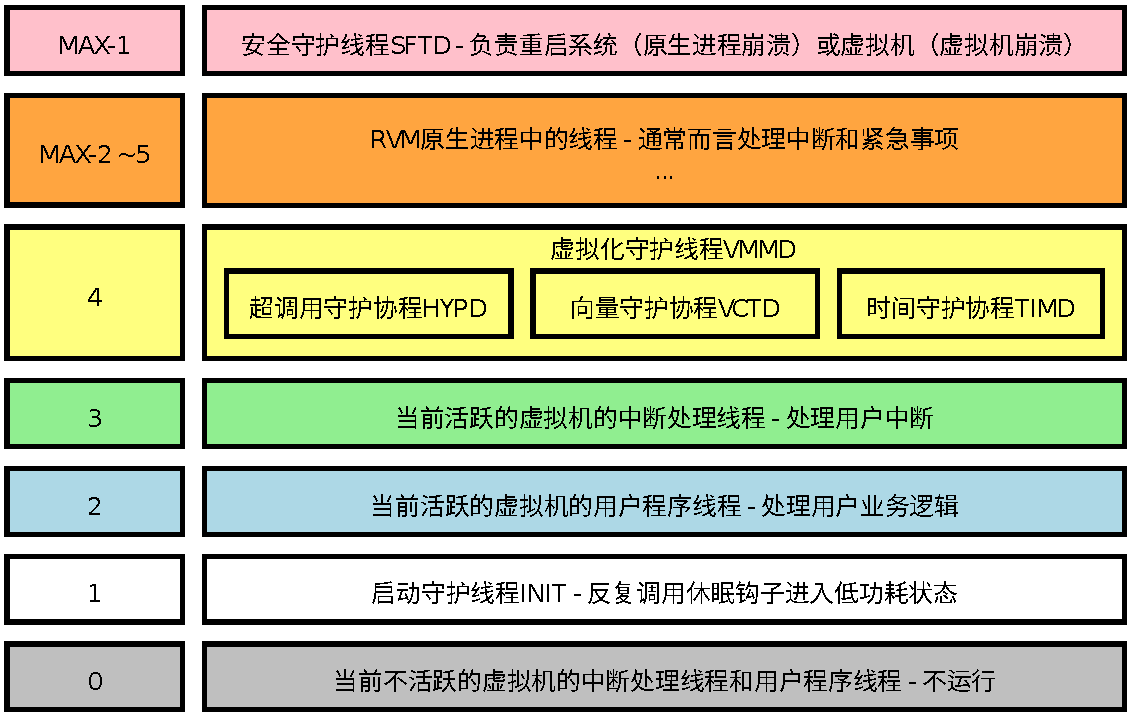
\includegraphics[width=0.90\textwidth]{Figure/image3.pdf}
\caption{虚拟化体系的中断优先级}\label{fig:2-2}
\end{figure}


各个虚拟机采用固定优先级时间片轮转法调度。它们之间的优先级则是由调度器守护线程决定的。为了系统安全，虚拟机的时间片和优先级是在系统编译时静态决定好的，RVM并不提供可以修改这两点的超级调用。这从根本上保证了虚拟机之间的时间隔离，使得没有虚拟机可以破坏整个系统的实时性。

\subsection{内存管理}\label{subsec:2-2-2}

在虚拟机中，最重要的事项之一就是内存管理。考虑到微控制器应用的一般特点，每个虚拟机的私有内存和共享内存，都是在编译时静态指定的。在系统开始运行之后，不再允许修改内存映射。对于每一种处理器，页表信息的格式都是不同的。请参看相应处理器的使用手册确定该处理器的页表形式。

手动构造和填充页表是非常繁琐的；为了避免不必要的麻烦，工程生成器提供了页表自动构造和填充的相关功能。

\subsection{CPU的虚拟化}\label{subsec:2-2-3}

在不同的准虚拟化平台中，CPU的虚拟化主要有两种主流设计策略，分别如下：

\begin{enumerate}
\def\labelenumi{{[}\arabic{enumi}{]}}
\item
  将每个虚拟机作为一个线程运行。这是专用准虚拟化平台最常见的解决方案，Xen即采取该策略。在每个客户机中，线程平时执行应用程序的代码；一旦设备中断或异常发生\footnote{在x86上，Xen利用了硬件特有的Ring1来加速系统调用和异常的处理，并不经过Xen，但设备中断依然需要经过Xen进行分发}，虚拟机监视器即强制修改线程的执行地址，迫使其执行一段中断处理代码，待处理结束后该线程自行返回应用程序中执行。在虚拟机监视器看来，此种方法最为方便，一方面每个客户机只有一个执行上下文，另一方面激活中断只要修改该上下文的指令指针。然而，在客户机看来，中断结束（End-Of-Interrupt，EOI）是否需要特意通知虚拟机监视器的问题会变得很难处理。这里主要有两种情况：相对简单的（1）虚拟机监视器一旦迫使某客户机执行虚拟中断向量，在客户机使用专用的超级调用通知虚拟机监视器当前中断已结束之前，虚拟机监视器不得再修改指令指针以迫使虚拟机执行中断向量，和较为复杂的（2）虚拟机监视器会无视客户机是否正在执行虚拟中断向量而总是修改指令指针迫使虚拟机执行中断向量。在情况（1）中，客户机端需要调用超级调用来通知虚拟机，这无疑增加了一次超级调用。对于直接运行在特权态的原生型虚拟机监视器Xen而言，一次超级调用就是一次上下文切换，开销还是可以忍受的；对于运行在用户态的宿主型虚拟机监视器RVM而言，一次超级调用意味着两次上下文切换，引入的延迟就不可忽视了。如果采取情况（2）中的解决方案，则更加糟糕：这意味着中断向量入口是必须可重入的，因此需要一段非常特殊的汇编代码。这段代码必须负责在重入的执行实例执行到真正的中断向量之前识别重入且在此后主动退出，在退出的过程中还要涉及对栈框的修补以使执行流带着正确的栈指针返回正在执行的中断向量。一方面这段代码非常难以正确编写\footnote{对五花八门的非标准嵌入式架构就更是如此}，另一方面它的开头总是大片的压栈。如果发生一系列紧密连续的中断，开头的压栈代码就会在来得及进行栈框修补之前重入多次，在嵌入式环境下会导致潜在的栈溢出。因此，即便（2）在Xen中非常高效，我们也不采用这种方式。
\item
  将每个客户机中的每个线程都作为一个独立的虚拟机线程运行。这是基于微内核的虚拟化的常见方案，L4Linux即采用该策略\protect\hyperref[cite:2-2]{{[}2{]}}。在微控制器上，这种策略的问题是（1）需要将原客户机操作系统的线程接口想办法对接到微内核的系统调用，这需要充分理解原操作系统的设计，甚至可能涉及到线程控制块等架构不相关部分的修改，（2）将每一个客户机线程都对应到微内核线程会导致创建出大量的微内核线程对象，这在Linux等线程结构本就庞大的重量级操作系统中是没有问题的，但在线程普遍极为轻量的RTOS中就等于成倍放大了存储器消耗，（3）微内核的线程切换需要经过一系列操作权能检查、时间预算检查和保护域切换检查，而甚至不具备保护域的RTOS线程根本用不着这些检查，每次都调用微内核系统调用来进行线程切换相当于成倍放大了执行时间消耗，在那些把时间资源作为独立可分配资源的微内核\footnote{如Composite和某些L4变体等}上就更是如此。

  为了解决上面的困境，RVM采用双线程的方法进行客户机的CPU虚拟化。每个客户机都具有Vct和Usr两个线程，Vct线程负责中断处理，Usr线程则负责处理用户程序。Vct平时不运行，只有当接收到了来自RVM的中断触发信号时才运行。当中断处理完成后，Vct又阻塞，Usr开始运行。Vct到Usr的切换利用了微内核的高效异步信号机制，不涉及RVM，因此比超级调用快得多。

  在Usr被切换走时，其寄存器组会被保存在由Reg\_Base\footnote{请参见\protect4.2}指定的地址。因此，要在Vct中修改Usr的寄存器组，只要修改那个地址上的寄存器数据即可。利用这个方法，可以在无需理解原RTOS设计的基础上对其硬件抽象层、尤其是其线程切换汇编进行逐行替换，从而轻松模拟RTOS中非常常见的线程上下文切换。
\end{enumerate}

\subsection{中断的虚拟化}\label{subsec:2-2-4}

对于虚拟机而言，中断虚拟化是必不可少的。RVM的每个客户机中都具有一个中断处理线程Vct，该线程的优先级比处理用户程序的Usr线程要高。该线程平时阻塞在各个虚拟机专属的虚拟中断向量端点上\footnote{该端点在每个虚拟机内部都位于权能号1的位置}，直到收到RVM发来的虚拟中断信号才被唤醒运行。

系统中的中断大概可以分成三类，第一类是时钟中断，它负责向操作系统提供时钟嘀嗒；第二类是线程切换中断，它负责进行RTOS的线程切换；第三类则是其他系统中断，它们负责响应其他外设的事务。这三类中断的特点也不同：时钟中断是周期性频繁发生的；线程切换中断本质上是自己发送给自己的软中断；其他系统中断则是不时发生的无规律中断。因此，RVM对于这三种中断采取了不同的虚拟化策略。

每个虚拟机都维护一个RVM\_State数据结构，其地址被State\_Base\footnote{请参见\protect4.2}指定。其内部的域如下：

\begin{xltabular}{\textwidth}{@{}>{\hsize=0.4500\hsize\raggedright\arraybackslash}X>{\hsize=1.5500\hsize\raggedright\arraybackslash}X@{}}
\caption{struct RVM\_\allowbreak{}State中各个域的意义}\label{tab:2-3}\\
\toprule
域名称 & 作用\tabularnewline
\endfirsthead
\toprule
域名称 & 作用\tabularnewline
\midrule
\endhead
\bottomrule
\endlastfoot
ptr\_\allowbreak{}t Vct\_\allowbreak{}Act &
指示当前虚拟机中运行的线程。如果置1，说明Vct线程正在运行，否则说明Usr线程正在运行。\tabularnewline
struct RVM\_\allowbreak{}Param Vct & Vct线程专用的超级调用参数区。\tabularnewline
struct RVM\_\allowbreak{}Param Usr & Usr线程专用的超级调用参数区。\tabularnewline
struct RVM\_\allowbreak{}Vctf Flag &
指示当前虚拟机中被激活的虚拟中断向量。\tabularnewline
\end{xltabular}

在该数据结构中，与中断虚拟化相关的数据结构为struct RVM\_Vctf Flag，它的各个域如下表所示。关于其它域，请参见\protect\hyperref[subsec:2-2-6]{2.2.6}
。

\begin{xltabular}{\textwidth}{@{}>{\hsize=0.4500\hsize\raggedright\arraybackslash}X>{\hsize=1.5500\hsize\raggedright\arraybackslash}X@{}}
\caption{struct RVM\_\allowbreak{}Vctf中各个域的意义}\label{tab:2-4}\\
\toprule
域名称 & 作用\tabularnewline
\endfirsthead
\toprule
域名称 & 作用\tabularnewline
\midrule
\endhead
\bottomrule
\endlastfoot
ptr\_\allowbreak{}t Tim & 指示时钟中断激活。\tabularnewline
ptr\_\allowbreak{}t Ctx & 指示线程切换中断激活。\tabularnewline
u8\_\allowbreak{}t Vct{[}{]} &
指示其它虚拟中断向量激活。每个字节对应一个虚拟中断向量。\tabularnewline
\end{xltabular}

在该数据结构中，时钟中断和线程切换中断的激活由两个单独的机器字指示，其它虚拟中断向量则每个对应于一个字节。当对应的中断被激活时，相应的域就被置1。这里不采取一个二进制位对应一个中断向量的方法，这样就不需要原子逻辑与指令\footnote{VCTD在置位某个向量时，Vct线程可能正在复位其中的某个向量。如果采取每个二进制位对应一个中断向量，则Vct线程必须使用原子逻辑与操作来复位标志位。部分架构，如ARMv6-M，是没有这种原子操作的，因此一个字节对应一个标志兼容性更好。}。由于每个虚拟机的虚拟中断向量数都有限，所以造成的存储空间浪费是可以容忍的。

比如，若VCTD判定某虚拟机的4号中断向量被激活，它会将Vct{[}4{]}置1，并向该虚拟机的Vct线程的专属端点发送信号。收到该信号的Vct线程被激活后，会先扫描整个结构体，并通过Vct{[}4{]}被置1判断4号虚拟中断向量被激活。之后，Vct线程会先将Vct{[}4{]}清零，再调用用户使用RVM\_Virt\_Vct\_Reg\footnote{请参见\protect4.5.5}注册的4号虚拟中断向量。这样一来，即便用户注册的中断向量执行时有新的4号中断到来，也不会产生中断丢失，因为Vct{[}4{]}将重新置位：Vct线程将在下一个循环后检测到4号中断悬起并再次进入它。

虚拟机的中断开关，以及虚拟机的虚拟中断向量与对应物理中断向量或事件源的对应关系是可以通过超级调用设置的。有关这些超级调用的信息请参见\protect\hyperref[sec:4-4]{4.4}
。一个标准的虚拟机中断初始化流程是：

\begin{enumerate}
\def\labelenumi{{[}\arabic{enumi}{]}}
\item
  调用RVM\_Virt\_Tim\_Reg注册时钟中断，
\item
  调用RVM\_Virt\_Ctx\_Reg注册线程切换中断，
\item
  调用RVM\_Virt\_Vct\_Reg注册其它虚拟中断，
\item
  调用RVM\_Hyp\_Vct\_Phys将所需的物理中断源映射到虚拟中断源，
\item
  调用RVM\_Hyp\_Vct\_Evt将所需的事件源映射到虚拟中断源，
\item
  调用RVM\_Hyp\_Vct\_Lck将事件源映射锁死以防止后续篡改，
\item
  在合适的地方调用RVM\_Hyp\_Int\_Ena开启虚拟机总中断。如果虚拟机还使用看门狗，需要调用RVM\_Hyp\_Wdg\_Clr来启动看门狗。看门狗一经启动则无法关闭。
\item
  虚拟机内的RTOS在其空闲线程中应当反复调用RVM\_Hyp\_Vct\_Wait以使虚拟机在空闲时进入休眠，并等待下一次中断来临。如果虚拟机还使用看门狗，需要在合适的地方调用RVM\_Hyp\_Wdg\_Clr来喂狗。
\end{enumerate}

\subsubsection{定时器中断的虚拟化}\label{subsubsec:2-2-4-1}

在RVM上运行的RTOS按照对定时器的运用方式可以分为两类，分别是有节拍（Periodic）内核和无节拍（Tickless）内核。前者要求系统中具备一个周期性发送中断的自动重装（Auto-reload）定时器，后者则要求每次上下文切换时按需编程一个倒计时结束后发送中断的一次性（One-shot）定时器。在裸机上，后者在低功耗特性方面更加优越，因为在处理器休眠或仅调度一个任务时不产生时钟中断。为此，在那些支持无节拍内核的RTOS上，我们常常启用这个特性。

然而，在虚拟化环境中则正好相反。无节拍内核对定时器的编程不再能直接完成，而要通过超级调用求助RVM。这会导致在每次上下文切换时多出一个超级调用，从而造成难以忍受的性能和实时性开销。此外，并非所有的RTOS都支持无节拍内核模式：哪怕有一个有节拍内核运行在RVM上，RVM还是要周期性地被唤醒以发送定时器中断给它，从而不可能降低功耗；这让其它内核的无节拍特性变得徒增开销。退一步讲，即便运行在RVM上的一切虚拟机都是无节拍的，它们对定时器的编程次数的总和也会非常多，而RVM必须将硬件定时器的超时时间设置成所有时刻中的最小值。这会导致定时器总是在一小段时间后就被触发，也不太可能起到低功耗效果。

基于上述原因，RVM使用有节拍设计。它需要的周期性时钟信号由RME的底层定时器产生，并且通过RVM\_BOOT\_INIT\_TIM端点发送到RVM的时钟处理守护线程。该守护线程会计算当前经过的时间周期数，并且根据各个虚拟机配置的分频系数Period\footnote{请参见\protect4.2}给各个虚拟机发送时钟中断。

具体地，Vct线程将调用用户使用RVM\_Virt\_Tim\_Reg\footnote{请参见\protect4.5.7}注册的线程切换钩子Tim。该钩子函数可以直接使用原裸机RTOS的定时器中断向量，且在需要时可使用RVM\_Virt\_Yield\footnote{请参见\protect4.5.7}来触发上下文切换\footnote{就好像在原RTOS中触发PendSV等上下文切换中断那样}。

\subsubsection{线程切换中断的虚拟化}\label{subsubsec:2-2-4-2}

线程切换中断本质上是一个软中断，它来源于虚拟机自身的内部。这个中断的响应效率将直接决定虚拟机的线程切换时间，因此保证它的效率非常重要。为此，RVM被特别设计为可以由用户线程Usr在不经过虚拟机监视器介入的情况下使用RVM\_Virt\_Yield\footnote{请参见\protect4.5.7}直接触发Vct线程主导的上下文切换，且在Vct线程中可直接修改提前映射到Reg\_Base\footnote{请参见\protect4.2}的Usr寄存器组，无需再使用任何系统调用。这个实现最大限度地贴近了常见RTOS的线程切换语义，大大降低了虚拟机内部的线程切换开销。

具体地，Vct线程将调用用户使用RVM\_Virt\_Ctx\_Reg\footnote{请参见\protect4.5.7}注册的线程切换钩子Ctx。在该钩子中将实现对Usr的各个寄存器的保存和恢复，从而完成RTOS线程的切换。常见的线程切换手段包括两个步骤，（1）将一切寄存器压到老线程栈上，（2）再从新线程栈上恢复一切寄存器；这个过程在裸机RTOS中通常是由汇编语言完成的。在RVM中，实现该流程的Ctx钩子则可由C语言写成\footnote{具体例子可以参见RMP的RVM移植}。

与裸机RTOS不同，寄存器的保存和恢复必须包括Usr线程使用的超级调用参数缓冲区，它位于struct
RVM\_State结构体的struct RVM\_Param
Usr域。这是因为，Usr线程对应的多个RTOS线程可能会并发访问它\footnote{比如它们同时进行超级调用}。关于该域的详细信息，请参见\protect\hyperref[subsec:2-2-6]{2.2.6}
。

\subsubsection{其他中断的虚拟化}\label{subsubsec:2-2-4-3}

由于不同的虚拟机需要接收不同的外设中断，因此其他外设中断要按需送往各个虚拟机。因此，系统提供了调用接口来让各个虚拟机设置自己的每个虚拟中断向量对应的物理中断源。每个虚拟机能且只能设置自己的虚拟中断向量对应的物理中断源。一旦该物理中断被触发，登记于这个物理中断上的所有的虚拟机的相应虚拟中断向量均会收到此中断。虚拟中断源的编号越小，其优先级就越高，但虚拟中断之间不会发生抢占和嵌套。

各虚拟中断对应的中断处理向量可以注册为不可掩蔽的``透明中断''或可掩蔽的``可感知中断''\footnote{这模拟了ARMv7-M等的PRIMASK功能，允许客户机在锁调度器时响应与RTOS无关的中断，提高了实时性}。前者在中断被掩蔽时仍会被响应，后者在中断被掩蔽时则不会被响应。定时器中断和线程切换中断则总是可掩蔽的。有关这些超级调用的信息，请参见\protect\hyperref[sec:4-4]{4.4}
。

\subsection{设备的虚拟化}\label{subsec:2-2-5}

在不同的虚拟化平台中，设备及其驱动的虚拟化主要有四种主流设计策略，分别如下：

\begin{enumerate}
\def\labelenumi{{[}\arabic{enumi}{]}}
\item
  将设备驱动放进一个单独的、具备特权虚拟机Dom0中，其余虚拟机通过向该虚拟机发送请求来访问设备。这是Xen等原生型虚拟机监视器常采取的策略\protect\hyperref[cite:2-1]{{[}1{]}}。采取这种策略的动力很好理解：（1）将设备直接交给虚拟机是无法安全共享的，要将它们与虚拟机隔离就需要将其放进单独的保护域，而虚拟机监视器提供了虚拟机作为隔离手段，（2）客户机操作系统中已有现成的驱动，单独为虚拟机监视器再准备一套驱动无异于重造轮子。然而，这种策略使任何设备I/O都包含昂贵的虚拟机间上下文切换，性能开销极大。此外，一旦虚拟机监视器对Dom0的中断调度或分发不当，其延迟将会扩散到整个系统中，造成毁灭性的实时性问题\protect\hyperref[cite:2-3]{{[}3{]}}。因此，RVM不能采取这种策略。
\item
  将设备驱动放在虚拟机监视器所在的内核态中。这是VMware ESXi等原生虚拟机监视器采取的另一种策略。这种方案可以完全规避掉Dom0的性能问题，但它将虚拟机监视器------也即整个系统的可信计算基------置于恶意驱动的威胁之下。显然，只有在虚拟机监视器厂商对驱动非常自信的情况下才能这样做，而且第三方设备厂商还必须配合这种认证。在微控制器中这些条件都不存在，因此RVM不能采取这种策略。
\item
  将虚拟机监视器和操作系统内核做成一个，这样客户机自然就能享受操作系统自带的设备驱动。这是KVM等虚拟机监视器通常采取的策略。它和上一种策略实际上或多或少是同样的，只不过驱动程序的开发者普遍认为开发工作是给Linux做的，因而积极性相对较高。
\item
  将各个驱动程序直接放置在各客户机中。这是很多工业场景和功能安全场景下的解决方案，因为工业场景下的每个虚拟机往往是各司其职\footnote{可以说是沿功能的分界面进行``纵切''，而非像大多数系统那样沿抽象层次的分界面进行``横切''}，各客户机间的功能重叠面很小，硬件的共享面也很小。利用工业嵌入式场景的这个特性，这个方案在设备划分得当时往往非常高效，因为虚拟机监视器将不再介入除中断分发之外的任何设备操作。然而，这种方案要求（1）任何设备的错误甚至是恶意操作都不得对系统安全和实时性造成威胁，包括那些往往被忽视的、由侧信道引起的问题\footnote{最典型的是DMA控制器，允许不可信虚拟机任意操作它可以轻易绕过所有安全机制}，（2）任何设备都只能被一个虚拟机独占，无法在虚拟机间进行任何设备共享，而且（3）中断仍然要传递到虚拟机中才可以处理，实时性不够。因此，这种方案不是总能使用。

  考虑到微控制器的实际情况，RVM鼓励在任何可能的时候使用方案4。如果实时性不够，或者需要共享设备，可以考虑将驱动程序的简单、可信赖的上半部\footnote{通常只包括寄存器的简单读写以及消息队列的发送}放置在中断响应极快的原生进程中，而将其下半部和协议栈放置在客户机中。原生进程可以和客户机都共享一部分内存以用于传递数据，且在共享时要保证客户机不破坏原生进程中线程执行所必要的数据。
\end{enumerate}

\subsection{超级调用的设计}\label{subsec:2-2-6}

虚拟机可以通过超级调用向虚拟机监视器请求服务。有关这些超级调用的信息，请参见\protect\hyperref[sec:4-4]{4.4}
。要发起超级调用，虚拟机会先将超级调用所需的各个参数写到与RVM约定好的参数缓冲区，然后向HYPD的信号端点RVM\_Hypd\_Sig\_Cap发送信号\footnote{该端点在每个虚拟机内部都位于权能号0的位置}。该参数缓冲区位于RVM\_State数据结构中，且存在两份：struct
RVM\_Param Vct为Vct线程专用，而struct RVM\_Param
Usr为Usr线程专用，这样就可以防止Vct线程和Usr线程在参数缓冲区上产生竞争冒险。

HYPD在收到超级调用后，会通过RVM\_State数据结构中的Vct\_Act判断当前正在运行的线程。如果Vct\_Act为1，说明当前运行的是Vct线程，超级调用参数应当从Vct线程的参数缓冲区中提取；否则说明当前运行的是Usr线程，超级调用参数应当从Usr线程的参数缓冲区中提取。在执行完超级调用之后，HYPD会将返回值写回对应的参数缓冲区；虚拟机在重新获得运行权后将提取该值作为超级调用的返回值。

由于一个Usr线程对应的多个RTOS线程同时也可能并发访问Usr线程的参数缓冲区，因此在RTOS的线程切换中，Usr线程使用的参数缓冲区将和寄存器组一起压栈弹栈，这确保了不会发生竞争冒险。

\subsection{跨保护域通信}\label{subsec:2-2-7}

为安全起见，原生进程与原生进程之间、原生进程与虚拟机之间，以及虚拟机与虚拟机之间是默认无法互相发送信号的。要使它们可以互相通信，需要做一些配置以在各个保护域中置入合适的信号原语。

\subsubsection{从原生进程发送信号到原生进程}\label{subsubsec:2-2-7-1}

原生进程之间可以通过RME的异步信号机制来进行通信。一个进程中的线程在信号端点上阻塞后，另一个进程中的线程只要向该端点发送信号就可以将阻塞解除。这要求一个进程具备端点的接收权能，另一个进程具备端点的发送权能。相关信息请参见\protect\hyperref[subsec:3-5-6]{3.5.6}
。

工程生成器可以根据用户对原生进程的描述正确地生成这种权能布局。只需要在接收的进程中声明接收端点，然后在发送的进程中向该端点发送就可以了。

\subsubsection{从虚拟机发送信号到原生进程}\label{subsubsec:2-2-7-2}

若要从虚拟机发送给原生进程，则可直接在原生进程中声明接收信号端点，并在虚拟机中声明发送信号端点，由虚拟机直接向原生进程发起信号发送即可。相关信息请参见\protect\hyperref[subsec:3-5-6]{3.5.6}
。

工程生成器允许在虚拟机中引用任何原生进程中声明的接收端点，并能够在系统启动时将对应的端点发送权限正确赋予虚拟机；虚拟机只需要向该端点发送就可以了。

\subsubsection{原生进程或虚拟机发送信号到虚拟机}\label{subsubsec:2-2-7-3}

由于虚拟机的Vct和Usr线程是不允许阻塞在信号端点上的，虚拟机内也无法定义信号端点发送权限之外的任何其它内核对象，从其它保护域\footnote{无论该保护域是原生进程还是虚拟机}到虚拟机的通信只能采取激活虚拟中断的方法。为此，RVM引入了``事件源''的概念\footnote{和常规的物理中断源一样，事件源也是一种全局刺激来源}：每个虚拟机都可以将自己的虚拟中断向量通过RVM\_Hyp\_Vct\_Evt自由注册到事件源，该事件源一旦激活，注册了该中断源的虚拟机就都会收到该虚拟中断。

原生进程的优先级高于虚拟机，因此限制它们对事件源的发送没有意义\footnote{它们只需要一直抢占处理器就可以阻止虚拟机监视器以及虚拟机的运行，因此限制它们没有意义}。虚拟机与虚拟机之间则并非如此：在虚拟机启动后，首先要通过RVM\_Hyp\_Evt\_Add函数事先申请向事件源进行发送的权限，并在申请完成后使用RVM\_Hyp\_Vct\_Lck将所有的事件源发送权限\footnote{以及事件源/中断源到虚拟中断之间的映射关系}锁死，在锁死后则不再允许对权限进行任何修改。此设计是基于这样一个假设：此后，通过RVM\_Hyp\_Evt\_Snd即可向事件源进行发送。相关信息请参见\protect\hyperref[sec:4-4]{4.4}
。

若要从虚拟机发送给原生进程，则可直接在原生进程中声明接收信号端点，并在虚拟机中声明发送信号端点，由虚拟机直接向原生进程发起信号发送即可。有关这些函数，请参见\protect\hyperref[subsec:3-5-6]{3.5.6}
。

事件源的总数量和事件源/物理中断源到虚拟中断的映射总数在工程生成器中可以配置，它是在工程编译前就静态决定好的；具体的映射关系则是在运行时动态建立的。

\needspace{12\baselineskip}
\section{本章参考文献}\label{sec:2-3}

\begin{enumerate}
\def\labelenumi{{[}\arabic{enumi}{]}}
\item
  \protect\phantomsection\label{cite:2-1}
  D. Chisnall, \textit{The Definitive Guide to the Xen Hypervisor}.
  Prentice Hall Open Source Software Development Series. Upper Saddle
  River, NJ, USA: Prentice Hall, 2008.
\item
  \protect\phantomsection\label{cite:2-2}
  A. Lackorzynski, ``L4Linux porting optimizations,'' Master's thesis.
\item
  \protect\phantomsection\label{cite:2-3}
  S. Yoo, K.-H. Kwak, J.-H. Jo, and C. Yoo, ``Toward under-millisecond
  I/O latency in Xen-ARM,'' in \textit{Proceedings of the Second
  Asia-Pacific Workshop on Systems}, Shanghai, China: ACM, 2011.
\end{enumerate}


\chapter{原生进程}\label{ch:3-native-process}

\section{简介}\label{sec:3-1}

原生进程直接运行在RME微内核之上，因此其运行速度最快，开销最小。RVM虚拟机监视器仅仅负责用INIT启动它们，而不能对它们提供任何服务。因此，原生进程仅能使用RME本身的系统调用，不能使用RVM超级调用。为了方便用户使用RME系统调用，RVM提供的用户态库对它们做了C语言接口封装。这些接口都是线程安全的。

工程生成器可以生成包含原生进程的工程。一个工程甚至可以仅仅包含原生进程，此时需要用原生进程直接完成应用程序的功能。

\section{进程描述符}\label{sec:3-2}

每一个原生进程（和虚拟机）都有一个位于其首部的进程描述符，该头部记载了进程中的每一个可能的入口点。这些入口点被虚拟机监视器识别，以用来初始化其内部数据结构。进程头的组成如下表所示。

\begin{xltabular}{\textwidth}{@{}>{\hsize=0.4500\hsize\raggedright\arraybackslash}X>{\hsize=1.5500\hsize\raggedright\arraybackslash}X@{}}
\caption{进程描述符的结构}\label{tab:3-1}\\
\toprule
地址（字） & 内容\tabularnewline
\endfirsthead
\toprule
地址（字） & 内容\tabularnewline
\midrule
\endhead
\bottomrule
\endlastfoot
0 &
魔法数字，对于原生进程而言是0x49535953，对于虚拟机而言是0x56495254。\tabularnewline
1 & 进程头的入口表项数N。\tabularnewline
2 & 第0个入口表项。\tabularnewline
3 & 第1个入口表项。\tabularnewline
... & ...\tabularnewline
N+1 & 第N-2个入口表项。\tabularnewline
N+2 &
第N-1个表项，固定存放跳板。在常规架构上，该项无用；在那些从栈中恢复PC的架构\footnote{如ARMv7-M}上，一段跳板是必须的，该跳板负责跳转程序到真正的入口点去执行。有关该跳板的描述请参见\protect8.2.6.2
。\tabularnewline
\end{xltabular}

工程生成器可以生成此进程描述符，当然也可以手动对其进行填充。

\section{登记原生进程到RVM}\label{sec:3-3}

要登记原生进程到RVM，需要用户手动使用RME系统调用创建其权能表、页表，以及其内部可能使用到的所有内核对象，并将进程内部可以使用的内核对象的权能全部传递到该进程的权能表内部。当权限关系十分复杂时，这是十分繁琐、容易出错的。工程生成器可以生成高度优化的数据结构自动完成上述流程，大大降低配置负担。如果需要手动完成该过程，可以重写rvm\_init.c中的如下两个钩子函数，并在其内部分别创建和初始化各个内核对象。

\subsection{内核对象创建钩子}\label{subsec:3-3-1}

用户应当在本钩子内部创建所有的内核对象。

\begin{xltabular}{\textwidth}{@{}>{\hsize=0.4500\hsize\raggedright\arraybackslash}X>{\hsize=1.5500\hsize\raggedright\arraybackslash}X@{}}
\caption{内核对象创建钩子}\label{tab:3-2}\\
\toprule
函数原型 & void RVM\_\allowbreak{}Boot\_\allowbreak{}Kobj\_\allowbreak{}Crt(void)\tabularnewline
\endfirsthead
\toprule
函数原型 & void RVM\_\allowbreak{}Boot\_\allowbreak{}Kobj\_\allowbreak{}Crt(void)\tabularnewline
\midrule
\endhead
\bottomrule
\endlastfoot
返回值 & 无。\tabularnewline
参数 & 无。\tabularnewline
\end{xltabular}

\subsection{内核对象初始化钩子}\label{subsec:3-3-2}

用户应当在本钩子内部初始化所有的内核对象。

\begin{xltabular}{\textwidth}{@{}>{\hsize=0.4500\hsize\raggedright\arraybackslash}X>{\hsize=1.5500\hsize\raggedright\arraybackslash}X@{}}
\caption{内核对象初始化钩子}\label{tab:3-3}\\
\toprule
函数原型 & void void RVM\_\allowbreak{}Boot\_\allowbreak{}Kobj\_\allowbreak{}Init(void)\tabularnewline
\endfirsthead
\toprule
函数原型 & void void RVM\_\allowbreak{}Boot\_\allowbreak{}Kobj\_\allowbreak{}Init(void)\tabularnewline
\midrule
\endhead
\bottomrule
\endlastfoot
返回值 & 无。\tabularnewline
参数 & 无。\tabularnewline
\end{xltabular}

\section{原生进程内应当存在的宏定义}\label{sec:3-4}

原生进程内部需要存在如下的配置宏定义，它们被原生进程内部的其他文件引用。这些宏定义可以由工程生成器负责填充，也可以由用户手动填充。这些宏定义的列表如下。

\begin{xltabular}{\textwidth}{@{}>{\hsize=0.4500\hsize\raggedright\arraybackslash}X>{\hsize=1.5500\hsize\raggedright\arraybackslash}X@{}}
\caption{原生进程内应当存在的宏定义一览}\label{tab:3-4}\\
\toprule
宏名称 & 作用\tabularnewline
\endfirsthead
\toprule
宏名称 & 作用\tabularnewline
\midrule
\endhead
\bottomrule
\endlastfoot
RVM\_\allowbreak{}VIRT\_\allowbreak{}LIB\_\allowbreak{}ENABLE\strut
 & 准虚拟化库的使能宏。在原生进程内它应当被定义为1。

例子：

\#define RVM\_\allowbreak{}VIRT\_\allowbreak{}LIB\_\allowbreak{}ENABLE (0U)\strut
\tabularnewline
RVM\_\allowbreak{}PREEMPT\_\allowbreak{}PRIO\_\allowbreak{}NUM\strut
 & 内核的优先级数量。它应当与RME中的同名配置宏维持一致。

例子：

\#define RVM\_\allowbreak{}PREEMPT\_\allowbreak{}PRIO\_\allowbreak{}NUM (4U)\strut
\tabularnewline
RVM\_\allowbreak{}PREEMPT\_\allowbreak{}VPRIO\_\allowbreak{}NUM\strut
 & 虚拟机监视器的虚拟优先级数量。它应当与虚拟机监视器配置中的值一致。

例子：

\#define RVM\_\allowbreak{}PREEMPT\_\allowbreak{}VPRIO\_\allowbreak{}NUM (32U)\strut
\tabularnewline
RVM\_\allowbreak{}KOM\_\allowbreak{}SLOT\_\allowbreak{}ORDER\strut
 & 内核内存分配粒度级数。它应当与RME中的同名配置宏维持一致。

例子：

\#define RVM\_\allowbreak{}KOM\_\allowbreak{}SLOT\_\allowbreak{}ORDER (4U)\strut
\tabularnewline
RVM\_\allowbreak{}ASSERT\_\allowbreak{}ENABLE\strut
 & 控制断言宏是否默认通过。如果它定义为0，则不再检查断言。

例子：

\#define RVM\_\allowbreak{}ASSERT\_\allowbreak{}ENABLE (1U)\strut
\tabularnewline
RVM\_\allowbreak{}DBGLOG\_\allowbreak{}ENABLE\strut
 & 控制调试打印的开关。如果它定义为0，则不再调试打印。

例子：

\#define RVM\_\allowbreak{}DBGLOG\_\allowbreak{}ENABLE (1U)\strut
\tabularnewline
\end{xltabular}

\section{原生进程可以使用的系统调用}\label{sec:3-5}

RME提供的所有系统调用都可以直接在原生进程中使用。这些系统调用的实现的通用部分都位于Guest文件夹下的rmv\_guest.c和rvm\_guest.h中，架构相关部分则位于子文件夹的rvm\_guest\_xxx.c，rvm\_guest\_xxx.h，rvm\_guest\_xxx\_conf.h中。下面仅对这些系统调用做简单描述；有关这些系统调用的具体信息，请查看RME的手册。

\subsection{权能表相关系统调用}\label{subsec:3-5-1}

这些接口向外提供了这些权能表相关调用的C语言接口。具体的函数列表如下所述：

\begin{xltabular}{\textwidth}{@{}>{\hsize=0.4500\hsize\raggedright\arraybackslash}X>{\hsize=1.5500\hsize\raggedright\arraybackslash}X@{}}
\caption{权能表相关系统调用}\label{tab:3-5}\\
\toprule
名称 & 接口函数原型\tabularnewline
\endfirsthead
\toprule
名称 & 接口函数原型\tabularnewline
\midrule
\endhead
\bottomrule
\endlastfoot
创建权能表\strut
 & ret\_\allowbreak{}t RVM\_\allowbreak{}Cpt\_\allowbreak{}Crt(cid\_\allowbreak{}t Cap\_\allowbreak{}Cpt\_\allowbreak{}Crt, cid\_\allowbreak{}t Cap\_\allowbreak{}Kom,

cid\_\allowbreak{}t Cap\_\allowbreak{}Cpt, ptr\_\allowbreak{}t Raddr, ptr\_\allowbreak{}t Entry\_\allowbreak{}Num)\strut
\tabularnewline
删除权能表 & ret\_\allowbreak{}t RVM\_\allowbreak{}Cpt\_\allowbreak{}Del(cid\_\allowbreak{}t Cap\_\allowbreak{}Cpt\_\allowbreak{}Del, cid\_\allowbreak{}t
Cap\_\allowbreak{}Del)\tabularnewline
传递普通权能\strut
 & ret\_\allowbreak{}t RVM\_\allowbreak{}Cpt\_\allowbreak{}Add(cid\_\allowbreak{}t Cap\_\allowbreak{}Cpt\_\allowbreak{}Dst, cid\_\allowbreak{}t Cap\_\allowbreak{}Dst,

cid\_\allowbreak{}t Cap\_\allowbreak{}Cpt\_\allowbreak{}Src, cid\_\allowbreak{}t Cap\_\allowbreak{}Src, ptr\_\allowbreak{}t Flag)

备注：该函数只能用来传递页目录权能、内核功能调用权能、内核内存权能之外的权能。\strut
\tabularnewline
传递页表权能\strut
 & ret\_\allowbreak{}t RVM\_\allowbreak{}Cpt\_\allowbreak{}Pgt(cid\_\allowbreak{}t Cap\_\allowbreak{}Cpt\_\allowbreak{}Dst, cid\_\allowbreak{}t Cap\_\allowbreak{}Dst,

cid\_\allowbreak{}t Cap\_\allowbreak{}Cpt\_\allowbreak{}Src, cid\_\allowbreak{}t Cap\_\allowbreak{}Src,

ptr\_\allowbreak{}t Begin, ptr\_\allowbreak{}t End, ptr\_\allowbreak{}t Flag)

备注：该函数不能被用来传递其他类型的权能。Begin和End两个参数标志了新的页表权能的起始槽位和终止槽位，也即其操作范围。该范围包括End。\strut
\tabularnewline
传递内核功能调用权能\strut
 & ret\_\allowbreak{}t RVM\_\allowbreak{}Cpt\_\allowbreak{}Kern(cid\_\allowbreak{}t Cap\_\allowbreak{}Cpt\_\allowbreak{}Dst, cid\_\allowbreak{}t Cap\_\allowbreak{}Dst,

cid\_\allowbreak{}t Cap\_\allowbreak{}Cpt\_\allowbreak{}Src, cid\_\allowbreak{}t Cap\_\allowbreak{}Src,

ptr\_\allowbreak{}t Begin, ptr\_\allowbreak{}t End)

备注：该函数不能被用来传递其他类型的权能。Begin和End两个参数标志了新的内核功能调用权能的起始槽位和终止槽位，也即其操作范围。该范围包括End。\strut
\tabularnewline
传递内核内存权能\strut
 & ret\_\allowbreak{}t RVM\_\allowbreak{}Cpt\_\allowbreak{}Kom(cid\_\allowbreak{}t Cap\_\allowbreak{}Cpt\_\allowbreak{}Dst, cid\_\allowbreak{}t Cap\_\allowbreak{}Dst,

cid\_\allowbreak{}t Cap\_\allowbreak{}Cpt\_\allowbreak{}Src, cid\_\allowbreak{}t Cap\_\allowbreak{}Src,

ptr\_\allowbreak{}t Begin, ptr\_\allowbreak{}t End, ptr\_\allowbreak{}t Flag)

备注：该函数不能被用来传递其他类型的权能。Begin和End两个参数标志了新的内核内存权能的起始地址和终止地址，它们被强制对齐到64Byte
。该范围不包括End。\strut
\tabularnewline
权能冻结 & ret\_\allowbreak{}t RVM\_\allowbreak{}Cpt\_\allowbreak{}Frz(cid\_\allowbreak{}t Cap\_\allowbreak{}Cpt\_\allowbreak{}Frz, cid\_\allowbreak{}t
Cap\_\allowbreak{}Frz)\tabularnewline
权能移除 & ret\_\allowbreak{}t RVM\_\allowbreak{}Cpt\_\allowbreak{}Rem(cid\_\allowbreak{}t Cap\_\allowbreak{}Cpt\_\allowbreak{}Rem, cid\_\allowbreak{}t
Cap\_\allowbreak{}Rem)\tabularnewline
\end{xltabular}

\subsection{内核功能相关系统调用}\label{subsec:3-5-2}

这些接口向外提供了这些内核功能相关调用的C语言接口。具体的函数列表如下所述：

\begin{xltabular}{\textwidth}{@{}>{\hsize=0.4500\hsize\raggedright\arraybackslash}X>{\hsize=1.5500\hsize\raggedright\arraybackslash}X@{}}
\caption{内核功能相关系统调用}\label{tab:3-6}\\
\toprule
名称 & 接口函数原型\tabularnewline
\endfirsthead
\toprule
名称 & 接口函数原型\tabularnewline
\midrule
\endhead
\bottomrule
\endlastfoot
内核调用激活\strut
 & ret\_\allowbreak{}t RVM\_\allowbreak{}Kfn\_\allowbreak{}Act(cid\_\allowbreak{}t Cap\_\allowbreak{}Kfn, ptr\_\allowbreak{}t Func\_\allowbreak{}ID,

ptr\_\allowbreak{}t Sub\_\allowbreak{}ID, ptr\_\allowbreak{}t Param1, ptr\_\allowbreak{}t Param2)\strut
\tabularnewline
\end{xltabular}

\newpage
\subsection{页表相关系统调用}\label{subsec:3-5-3}

这些接口向外提供了这些页表相关调用的C语言接口。具体的函数列表如下所述：

\begin{xltabular}{\textwidth}{@{}>{\hsize=0.4500\hsize\raggedright\arraybackslash}X>{\hsize=1.5500\hsize\raggedright\arraybackslash}X@{}}
\caption{页表相关系统调用}\label{tab:3-7}\\
\toprule
名称 & 接口函数原型\tabularnewline
\endfirsthead
\toprule
名称 & 接口函数原型\tabularnewline
\midrule
\endhead
\bottomrule
\endlastfoot
页目录创建\strut
 & ret\_\allowbreak{}t RVM\_\allowbreak{}Pgt\_\allowbreak{}Crt(cid\_\allowbreak{}t Cap\_\allowbreak{}Cpt, cid\_\allowbreak{}t Cap\_\allowbreak{}Kom, cid\_\allowbreak{}t Cap\_\allowbreak{}Pgt,

ptr\_\allowbreak{}t Raddr, ptr\_\allowbreak{}t Start\_\allowbreak{}Addr, ptr\_\allowbreak{}t Is\_\allowbreak{}Top,

ptr\_\allowbreak{}t Size\_\allowbreak{}Order, ptr\_\allowbreak{}t Num\_\allowbreak{}Order)\strut
\tabularnewline
删除页目录 & ret\_\allowbreak{}t RVM\_\allowbreak{}Pgt\_\allowbreak{}Del(cid\_\allowbreak{}t Cap\_\allowbreak{}Cpt, cid\_\allowbreak{}t
Cap\_\allowbreak{}Pgt)\tabularnewline
映射内存页\strut
 & ret\_\allowbreak{}t RVM\_\allowbreak{}Pgt\_\allowbreak{}Add(cid\_\allowbreak{}t Cap\_\allowbreak{}Pgt\_\allowbreak{}Dst, ptr\_\allowbreak{}t Pos\_\allowbreak{}Dst, ptr\_\allowbreak{}t
Flag\_\allowbreak{}Dst,

cid\_\allowbreak{}t Cap\_\allowbreak{}Pgt\_\allowbreak{}Src, ptr\_\allowbreak{}t Pos\_\allowbreak{}Src, ptr\_\allowbreak{}t Index)\strut
\tabularnewline
移除内存页 & ret\_\allowbreak{}t RVM\_\allowbreak{}Pgt\_\allowbreak{}Rem(cid\_\allowbreak{}t Cap\_\allowbreak{}Pgt, ptr\_\allowbreak{}t
Pos)\tabularnewline
构造页目录\strut
 & ret\_\allowbreak{}t RVM\_\allowbreak{}Pgt\_\allowbreak{}Con(cid\_\allowbreak{}t Cap\_\allowbreak{}Pgt\_\allowbreak{}Parent, ptr\_\allowbreak{}t Pos,

cid\_\allowbreak{}t Cap\_\allowbreak{}Pgt\_\allowbreak{}Child, ptr\_\allowbreak{}t Flags\_\allowbreak{}Childs)\strut
\tabularnewline
析构页目录 & ret\_\allowbreak{}t RVM\_\allowbreak{}Pgt\_\allowbreak{}Des(cid\_\allowbreak{}t Cap\_\allowbreak{}Pgt\_\allowbreak{}Parent, ptr\_\allowbreak{}t Pos,
cid\_\allowbreak{}t Cap\_\allowbreak{}Pgt\_\allowbreak{}Child)\tabularnewline
\end{xltabular}

\subsection{进程相关系统调用}\label{subsec:3-5-4}

这些接口向外提供了这些进程相关调用的C语言接口。具体的函数列表如下所述：

\begin{xltabular}{\textwidth}{@{}>{\hsize=0.4500\hsize\raggedright\arraybackslash}X>{\hsize=1.5500\hsize\raggedright\arraybackslash}X@{}}
\caption{进程相关系统调用}\label{tab:3-8}\\
\toprule
名称 & 接口函数原型\tabularnewline
\endfirsthead
\toprule
名称 & 接口函数原型\tabularnewline
\midrule
\endhead
\bottomrule
\endlastfoot
创建进程\strut
 & ret\_\allowbreak{}t RVM\_\allowbreak{}Prc\_\allowbreak{}Crt(cid\_\allowbreak{}t Cap\_\allowbreak{}Cpt\_\allowbreak{}Crt,

cid\_\allowbreak{}t Cap\_\allowbreak{}Prc, cid\_\allowbreak{}t Cap\_\allowbreak{}Cpt, cid\_\allowbreak{}t Cap\_\allowbreak{}Pgt)\strut
\tabularnewline
删除进程 & ret\_\allowbreak{}t RVM\_\allowbreak{}Prc\_\allowbreak{}Del(cid\_\allowbreak{}t Cap\_\allowbreak{}Cpt, cid\_\allowbreak{}t
Cap\_\allowbreak{}Prc)\tabularnewline
更改权能表 & ret\_\allowbreak{}t RVM\_\allowbreak{}Prc\_\allowbreak{}Cpt(cid\_\allowbreak{}t Cap\_\allowbreak{}Prc, cid\_\allowbreak{}t
Cap\_\allowbreak{}Cpt)\tabularnewline
更改页表 & ret\_\allowbreak{}t RVM\_\allowbreak{}Prc\_\allowbreak{}Pgt(cid\_\allowbreak{}t Cap\_\allowbreak{}Prc, cid\_\allowbreak{}t
Cap\_\allowbreak{}Pgt)\tabularnewline
\end{xltabular}

\subsection{线程相关系统调用}\label{subsec:3-5-5}

这些接口向外提供了这些线程相关调用的C语言接口。具体的函数列表如下所述：

\begin{xltabular}{\textwidth}{@{}>{\hsize=0.4500\hsize\raggedright\arraybackslash}X>{\hsize=1.5500\hsize\raggedright\arraybackslash}X@{}}
\caption{线程相关系统调用}\label{tab:3-9}\\
\toprule
名称 & 接口函数原型\tabularnewline
\endfirsthead
\toprule
名称 & 接口函数原型\tabularnewline
\midrule
\endhead
\bottomrule
\endlastfoot
创建线程\strut
 & ret\_\allowbreak{}t RVM\_\allowbreak{}Thd\_\allowbreak{}Crt(cid\_\allowbreak{}t Cap\_\allowbreak{}Cpt, cid\_\allowbreak{}t Cap\_\allowbreak{}Kom, cid\_\allowbreak{}t Cap\_\allowbreak{}Thd,

cid\_\allowbreak{}t Cap\_\allowbreak{}Prc, ptr\_\allowbreak{}t Max\_\allowbreak{}Prio, ptr\_\allowbreak{}t Raddr, ptr\_\allowbreak{}t Attr)\strut
\tabularnewline
创建虚拟机专用线程\footnote{除非要自行实现虚拟机监视器，否则不要调用}\strut
 & ret\_\allowbreak{}t RVM\_\allowbreak{}Hyp\_\allowbreak{}Crt(cid\_\allowbreak{}t Cap\_\allowbreak{}Cpt, cid\_\allowbreak{}t Cap\_\allowbreak{}Kom, cid\_\allowbreak{}t Cap\_\allowbreak{}Thd,

cid\_\allowbreak{}t Cap\_\allowbreak{}Prc, ptr\_\allowbreak{}t Max\_\allowbreak{}Prio, ptr\_\allowbreak{}t Raddr, ptr\_\allowbreak{}t Attr)\strut
\tabularnewline
删除线程 & ret\_\allowbreak{}t RVM\_\allowbreak{}Thd\_\allowbreak{}Del(cid\_\allowbreak{}t Cap\_\allowbreak{}Cpt, cid\_\allowbreak{}t
Cap\_\allowbreak{}Thd)\tabularnewline
设置执行属性 & ret\_\allowbreak{}t RVM\_\allowbreak{}Thd\_\allowbreak{}Exec\_\allowbreak{}Set(cid\_\allowbreak{}t Cap\_\allowbreak{}Thd, void* Entry,
void* Stack, void* Param)\tabularnewline
线程绑定\strut
 & ret\_\allowbreak{}t RVM\_\allowbreak{}Thd\_\allowbreak{}Sched\_\allowbreak{}Bind(cid\_\allowbreak{}t Cap\_\allowbreak{}Thd, cid\_\allowbreak{}t Cap\_\allowbreak{}Thd\_\allowbreak{}Sched,

cid\_\allowbreak{}t Cap\_\allowbreak{}Sig, tid\_\allowbreak{}t TID, ptr\_\allowbreak{}t Prio)\strut
\tabularnewline
虚拟机专用线程绑定\footnote{除非要自行实现虚拟机监视器，否则不要调用}\strut
 & ret\_\allowbreak{}t RVM\_\allowbreak{}Hyp\_\allowbreak{}Sched\_\allowbreak{}Bind(cid\_\allowbreak{}t Cap\_\allowbreak{}Thd, cid\_\allowbreak{}t Cap\_\allowbreak{}Thd\_\allowbreak{}Sched,

cid\_\allowbreak{}t Cap\_\allowbreak{}Sig, tid\_\allowbreak{}t TID, ptr\_\allowbreak{}t Prio, ptr\_\allowbreak{}t Haddr)\strut
\tabularnewline
更改优先级 & ret\_\allowbreak{}t RVM\_\allowbreak{}Thd\_\allowbreak{}Sched\_\allowbreak{}Prio(cid\_\allowbreak{}t Cap\_\allowbreak{}Thd, ptr\_\allowbreak{}t
Prio)\tabularnewline
更改优先级(2)\strut
 & ret\_\allowbreak{}t RVM\_\allowbreak{}Thd\_\allowbreak{}Sched\_\allowbreak{}Prio2(cid\_\allowbreak{}t Cap\_\allowbreak{}Thd0, ptr\_\allowbreak{}t Prio0,

cid\_\allowbreak{}t Cap\_\allowbreak{}Thd1, ptr\_\allowbreak{}t Prio1)

备注：一次可修改两个线程的优先级。\strut
\tabularnewline
更改优先级(3)\strut
 & ret\_\allowbreak{}t RVM\_\allowbreak{}Thd\_\allowbreak{}Sched\_\allowbreak{}Prio3(cid\_\allowbreak{}t Cap\_\allowbreak{}Thd0, ptr\_\allowbreak{}t Prio0,

cid\_\allowbreak{}t Cap\_\allowbreak{}Thd1, ptr\_\allowbreak{}t Prio1,

cid\_\allowbreak{}t Cap\_\allowbreak{}Thd2, ptr\_\allowbreak{}t Prio2)

备注：一次可修改三个线程的优先级。\strut
\tabularnewline
更改优先级(4)\strut
 & ret\_\allowbreak{}t RVM\_\allowbreak{}Thd\_\allowbreak{}Sched\_\allowbreak{}Prio4(cid\_\allowbreak{}t Cap\_\allowbreak{}Thd0, ptr\_\allowbreak{}t Prio0,

cid\_\allowbreak{}t Cap\_\allowbreak{}Thd1, ptr\_\allowbreak{}t Prio1,

cid\_\allowbreak{}t Cap\_\allowbreak{}Thd2, ptr\_\allowbreak{}t Prio2,

cid\_\allowbreak{}t Cap\_\allowbreak{}Thd3, ptr\_\allowbreak{}t Prio3)

备注：一次可修改四个线程的优先级。\strut
\tabularnewline
接收调度事件 & ret\_\allowbreak{}t RVM\_\allowbreak{}Thd\_\allowbreak{}Sched\_\allowbreak{}Rcv(cid\_\allowbreak{}t
Cap\_\allowbreak{}Thd)\tabularnewline
解除绑定 & ret\_\allowbreak{}t RVM\_\allowbreak{}Thd\_\allowbreak{}Sched\_\allowbreak{}Free(cid\_\allowbreak{}t Cap\_\allowbreak{}Thd)\tabularnewline
传递时间片 & ret\_\allowbreak{}t RVM\_\allowbreak{}Thd\_\allowbreak{}Time\_\allowbreak{}Xfer(cid\_\allowbreak{}t Cap\_\allowbreak{}Thd\_\allowbreak{}Dst, cid\_\allowbreak{}t
Cap\_\allowbreak{}Thd\_\allowbreak{}Src, ptr\_\allowbreak{}t Time)\tabularnewline
切换到某线程 & ret\_\allowbreak{}t RVM\_\allowbreak{}Thd\_\allowbreak{}Swt(cid\_\allowbreak{}t Cap\_\allowbreak{}Thd, ptr\_\allowbreak{}t
Is\_\allowbreak{}Yield)\tabularnewline
\end{xltabular}

\subsection{异步信号端点相关系统调用}\label{subsec:3-5-6}

这些接口向外提供了这些信号端点相关调用的C语言接口。具体的函数列表如下所述：

\begin{xltabular}{\textwidth}{@{}>{\hsize=0.4500\hsize\raggedright\arraybackslash}X>{\hsize=1.5500\hsize\raggedright\arraybackslash}X@{}}
\caption{异步信号端点相关系统调用}\label{tab:3-10}\\
\toprule
名称 & 接口函数原型\tabularnewline
\endfirsthead
\toprule
名称 & 接口函数原型\tabularnewline
\midrule
\endhead
\bottomrule
\endlastfoot
创建信号端点 & ret\_\allowbreak{}t RVM\_\allowbreak{}Sig\_\allowbreak{}Crt(cid\_\allowbreak{}t Cap\_\allowbreak{}Cpt, cid\_\allowbreak{}t
Cap\_\allowbreak{}Sig)\tabularnewline
删除信号端点 & ret\_\allowbreak{}t RVM\_\allowbreak{}Sig\_\allowbreak{}Del(cid\_\allowbreak{}t Cap\_\allowbreak{}Cpt, cid\_\allowbreak{}t
Cap\_\allowbreak{}Sig)\tabularnewline
向端点发送 & ret\_\allowbreak{}t RVM\_\allowbreak{}Sig\_\allowbreak{}Snd(cid\_\allowbreak{}t Cap\_\allowbreak{}Sig, ptr\_\allowbreak{}t
Number)\tabularnewline
从端点接收 & ret\_\allowbreak{}t RVM\_\allowbreak{}Sig\_\allowbreak{}Rcv(cid\_\allowbreak{}t Cap\_\allowbreak{}Sig, ptr\_\allowbreak{}t
Option)\tabularnewline
\end{xltabular}

\subsection{同步迁移调用相关系统调用}\label{subsec:3-5-7}

这些接口向外提供了这些线程迁移相关调用的C语言接口。具体的函数列表如下所述：

\begin{xltabular}{\textwidth}{@{}>{\hsize=0.4500\hsize\raggedright\arraybackslash}X>{\hsize=1.5500\hsize\raggedright\arraybackslash}X@{}}
\caption{同步迁移调用相关系统调用}\label{tab:3-11}\\
\toprule
名称 & 接口函数原型\tabularnewline
\endfirsthead
\toprule
名称 & 接口函数原型\tabularnewline
\midrule
\endhead
\bottomrule
\endlastfoot
创建同步迁移调用\strut
 & ret\_\allowbreak{}t RVM\_\allowbreak{}Inv\_\allowbreak{}Crt(cid\_\allowbreak{}t Cap\_\allowbreak{}Cpt, cid\_\allowbreak{}t Cap\_\allowbreak{}Kom,

cid\_\allowbreak{}t Cap\_\allowbreak{}Inv, cid\_\allowbreak{}t Cap\_\allowbreak{}Prc, ptr\_\allowbreak{}t Raddr)\strut
\tabularnewline
删除同步迁移调用 & ret\_\allowbreak{}t RVM\_\allowbreak{}Inv\_\allowbreak{}Del(cid\_\allowbreak{}t Cap\_\allowbreak{}Cpt, cid\_\allowbreak{}t
Cap\_\allowbreak{}Inv)\tabularnewline
设置执行属性\strut
 & ret\_\allowbreak{}t RVM\_\allowbreak{}Inv\_\allowbreak{}Set(cid\_\allowbreak{}t Cap\_\allowbreak{}Inv, ptr\_\allowbreak{}t Entry,

ptr\_\allowbreak{}t Stack, ptr\_\allowbreak{}t Is\_\allowbreak{}Exc\_\allowbreak{}Ret)\strut
\tabularnewline
激活同步迁移调用 & ret\_\allowbreak{}t RVM\_\allowbreak{}Inv\_\allowbreak{}Act(cid\_\allowbreak{}t Cap\_\allowbreak{}Inv, ptr\_\allowbreak{}t Param,
ptr\_\allowbreak{}t* Retval)\tabularnewline
从同步迁移调用返回 & ret\_\allowbreak{}t RVM\_\allowbreak{}Inv\_\allowbreak{}Ret(ptr\_\allowbreak{}t Retval)\tabularnewline
\end{xltabular}

\subsection{事件源激活相关系统调用}\label{subsec:3-5-8}

要从原生进程发送消息给虚拟机，可以使用RVM\_Prc\_Evt\_Snd函数来激活任何一个事件源，注册了该事件源的虚拟机均会得到一个虚拟中断。由于原生进程本身的优先级高于整个虚拟机子系统\footnote{这甚至包括了虚拟机监视器中除SFTD以外的一切线程}，因此本函数并对事件源目标加以限制，原生进程可自行决定发送信号给任意一个事件源。有关事件源，请参见\protect\hyperref[subsec:2-2-7]{2.2.7}
。

\begin{xltabular}{\textwidth}{@{}>{\hsize=0.5500\hsize\raggedright\arraybackslash}X>{\hsize=0.7500\hsize\raggedright\arraybackslash}X>{\hsize=1.5500\hsize\raggedright\arraybackslash}X@{}}
\caption{激活事件源的所需参数}\label{tab:3-12}\\
\toprule
原型 & ret\_\allowbreak{}t RVM\_\allowbreak{}Prc\_\allowbreak{}Evt\_\allowbreak{}Snd(ptr\_\allowbreak{}t Evt\_\allowbreak{}Num) &\tabularnewline
\endfirsthead
\toprule
原型 & ret\_\allowbreak{}t RVM\_\allowbreak{}Prc\_\allowbreak{}Evt\_\allowbreak{}Snd(ptr\_\allowbreak{}t Evt\_\allowbreak{}Num) &\tabularnewline
\midrule
\endhead
\bottomrule
\endlastfoot
参数名称 & 类型 & 描述\tabularnewline
Evt\_\allowbreak{}Num & ptr\_\allowbreak{}t & 事件源的编号。\tabularnewline
\end{xltabular}

\section{原生进程可以使用的其他助手函数}\label{sec:3-6}

为了方便常用数据结构编写、调试打印、线程栈初始化，RVM还提供了一些助手函数。下面列出的所有助手函数均可以在原生进程中使用。

\begin{xltabular}{\textwidth}{@{}>{\hsize=0.4500\hsize\raggedright\arraybackslash}X>{\hsize=1.5500\hsize\raggedright\arraybackslash}X@{}}
\caption{原生进程可以使用的其他助手函数一览}\label{tab:3-13}\\
\toprule
函数 & 意义\tabularnewline
\endfirsthead
\toprule
函数 & 意义\tabularnewline
\midrule
\endhead
\bottomrule
\endlastfoot
RVM\_\allowbreak{}Clear & 变量清空。\tabularnewline
RVM\_\allowbreak{}List\_\allowbreak{}Crt & 创建双向循环链表。\tabularnewline
RVM\_\allowbreak{}List\_\allowbreak{}Del & 在双向循环链表中删除节点。\tabularnewline
RVM\_\allowbreak{}List\_\allowbreak{}Ins & 在双向循环链表中插入节点。\tabularnewline
RVM\_\allowbreak{}Putchar & 打印单个字符。\tabularnewline
RVM\_\allowbreak{}Int\_\allowbreak{}Print & 打印整形数字。\tabularnewline
RVM\_\allowbreak{}Hex\_\allowbreak{}Print & 打印无符号整形数字。\tabularnewline
RVM\_\allowbreak{}Str\_\allowbreak{}Print & 打印字符串。\tabularnewline
\end{xltabular}

\subsection{变量清空}\label{subsec:3-6-1}

该函数用来在内核中清零一片区域。该函数实质上等价于C语言运行时库的memset函数填充0时的特殊情况。

\begin{xltabular}{\textwidth}{@{}>{\hsize=0.5500\hsize\raggedright\arraybackslash}X>{\hsize=0.7500\hsize\raggedright\arraybackslash}X>{\hsize=1.5500\hsize\raggedright\arraybackslash}X@{}}
\caption{变量清空的所需参数}\label{tab:3-14}\\
\toprule
原型 & void RVM\_\allowbreak{}Clear(volatile void* Addr, ptr\_\allowbreak{}t Size)
&\tabularnewline
\endfirsthead
\toprule
原型 & void RVM\_\allowbreak{}Clear(volatile void* Addr, ptr\_\allowbreak{}t Size)
&\tabularnewline
\midrule
\endhead
\bottomrule
\endlastfoot
参数名称 & 类型 & 描述\tabularnewline
Addr & volatile void* & 需要清零区域的起始地址。\tabularnewline
Size & ptr\_\allowbreak{}t & 需要清零区域的字节数。\tabularnewline
\end{xltabular}

\subsection{创建双向循环链表}\label{subsec:3-6-2}

本操作初始化双向循环链表的链表头。

\begin{xltabular}{\textwidth}{@{}>{\hsize=0.4500\hsize\raggedright\arraybackslash}X>{\hsize=1.5500\hsize\raggedright\arraybackslash}X@{}}
\caption{创建双向循环链表}\label{tab:3-15}\\
\toprule
函数原型 & void RVM\_\allowbreak{}List\_\allowbreak{}Crt(struct RVM\_\allowbreak{}List* Head)\tabularnewline
\endfirsthead
\toprule
函数原型 & void RVM\_\allowbreak{}List\_\allowbreak{}Crt(struct RVM\_\allowbreak{}List* Head)\tabularnewline
\midrule
\endhead
\bottomrule
\endlastfoot
返回值 & 无。\tabularnewline
参数\strut
 & struct RVM\_\allowbreak{}List* Head

指向要初始化的链表头结构体的指针。\strut
\tabularnewline
\end{xltabular}

\subsection{在双向循环链表中删除节点}\label{subsec:3-6-3}

本操作从双向链表中删除一个或一系列节点。

\begin{xltabular}{\textwidth}{@{}>{\hsize=0.4500\hsize\raggedright\arraybackslash}X>{\hsize=1.5500\hsize\raggedright\arraybackslash}X@{}}
\caption{在双向循环链表中删除节点}\label{tab:3-16}\\
\toprule
函数原型\strut
 & void RVM\_\allowbreak{}List\_\allowbreak{}Del(struct RVM\_\allowbreak{}List* Prev,

struct RVM\_\allowbreak{}List* Next)\strut
\tabularnewline
\endfirsthead
\toprule
函数原型\strut
 & void RVM\_\allowbreak{}List\_\allowbreak{}Del(struct RVM\_\allowbreak{}List* Prev,

struct RVM\_\allowbreak{}List* Next)\strut
\tabularnewline
\midrule
\endhead
\bottomrule
\endlastfoot
返回值 & 无。\tabularnewline
\multirow{2}{*}{参数} & struct RVM\_\allowbreak{}List* Prev

指向要删除的节点（组）的前继节点的指针。\strut
\tabularnewline
\strut
 & struct RVM\_\allowbreak{}List* Next

指向要删除的节点（组）的后继节点的指针。\strut
\tabularnewline
\end{xltabular}

\subsection{在双向循环链表中插入节点}\label{subsec:3-6-4}

本操作从双向链表中插入一个节点。

\begin{xltabular}{\textwidth}{@{}>{\hsize=0.4500\hsize\raggedright\arraybackslash}X>{\hsize=1.5500\hsize\raggedright\arraybackslash}X@{}}
\caption{在双向循环链表中插入节点}\label{tab:3-17}\\
\toprule
函数原型\strut
 & void RVM\_\allowbreak{}List\_\allowbreak{}Ins(struct RVM\_\allowbreak{}List* New,

struct RVM\_\allowbreak{}List* Prev,

struct RVM\_\allowbreak{}List* Next)\strut
\tabularnewline
\endfirsthead
\toprule
函数原型\strut
 & void RVM\_\allowbreak{}List\_\allowbreak{}Ins(struct RVM\_\allowbreak{}List* New,

struct RVM\_\allowbreak{}List* Prev,

struct RVM\_\allowbreak{}List* Next)\strut
\tabularnewline
\midrule
\endhead
\bottomrule
\endlastfoot
返回值 & 无。\tabularnewline
\multirow{3}{*}{参数} & struct RVM\_\allowbreak{}List* New

指向要插入的新节点的指针。\strut
\tabularnewline
\strut
 & struct RVM\_\allowbreak{}List* Prev

指向要被插入的位置的前继节点的指针。\strut
\tabularnewline
\strut
 & struct RVM\_\allowbreak{}List* Next

指向要被插入的位置的后继节点的指针。\strut
\tabularnewline
\end{xltabular}

\subsection{打印单个字符}\label{subsec:3-6-5}

本操作打印一个字符到控制台。该函数需要用户自行声明和实现。在该函数的实现中，通常只需要重定向其输出到某外设即可。如果不实现该函数，后文的一切调试打印函数都无法使用。工程生成器会在生成的进程文件中提供该函数的原型，用户只需要使用合适的内容来填充它。

\begin{xltabular}{\textwidth}{@{}>{\hsize=0.4500\hsize\raggedright\arraybackslash}X>{\hsize=1.5500\hsize\raggedright\arraybackslash}X@{}}
\caption{打印单个字符}\label{tab:3-18}\\
\toprule
函数原型 & ptr\_\allowbreak{}t RVM\_\allowbreak{}Putchar(char Char)\tabularnewline
\endfirsthead
\toprule
函数原型 & ptr\_\allowbreak{}t RVM\_\allowbreak{}Putchar(char Char)\tabularnewline
\midrule
\endhead
\bottomrule
\endlastfoot
意义 & 输出一个字符到控制台。\tabularnewline
返回值\strut
 & ptr\_\allowbreak{}t

总是返回0。\strut
\tabularnewline
参数\strut
 & char Char

要输出到系统控制台的字符。\strut
\tabularnewline
\end{xltabular}

\subsection{打印整形数字}\label{subsec:3-6-6}

本操作以包含符号的十进制打印一个机器字长的整形数字到调试控制台。该函数有一个受调试开关控制的同功能宏RVM\_DBG\_I。要使用这个函数，需要RVM\_Putchar在进程内被声明和实现。

\begin{xltabular}{\textwidth}{@{}>{\hsize=0.4500\hsize\raggedright\arraybackslash}X>{\hsize=1.5500\hsize\raggedright\arraybackslash}X@{}}
\caption{打印整形数字}\label{tab:3-19}\\
\toprule
函数原型 & cnt\_\allowbreak{}t RVM\_\allowbreak{}Int\_\allowbreak{}Print(cnt\_\allowbreak{}t Int)\tabularnewline
\endfirsthead
\toprule
函数原型 & cnt\_\allowbreak{}t RVM\_\allowbreak{}Int\_\allowbreak{}Print(cnt\_\allowbreak{}t Int)\tabularnewline
\midrule
\endhead
\bottomrule
\endlastfoot
返回值\strut
 & cnt\_\allowbreak{}t

返回打印的字符数量。\strut
\tabularnewline
参数\strut
 & cnt\_\allowbreak{}t Int

要打印的整形数字。\strut
\tabularnewline
\end{xltabular}

\subsection{打印无符号整形数字}\label{subsec:3-6-7}

本操作以无前缀十六进制打印一个机器字长的无符号整形数字到调试控制台。该函数有一个受调试开关控制的同功能宏RVM\_DBG\_H。要使用这个函数，需要RVM\_Putchar在进程内被声明和实现。

\begin{xltabular}{\textwidth}{@{}>{\hsize=0.4500\hsize\raggedright\arraybackslash}X>{\hsize=1.5500\hsize\raggedright\arraybackslash}X@{}}
\caption{打印无符号整形数字}\label{tab:3-20}\\
\toprule
函数原型 & cnt\_\allowbreak{}t RVM\_\allowbreak{}Hex\_\allowbreak{}Print(ptr\_\allowbreak{}t Uint)\tabularnewline
\endfirsthead
\toprule
函数原型 & cnt\_\allowbreak{}t RVM\_\allowbreak{}Hex\_\allowbreak{}Print(ptr\_\allowbreak{}t Uint)\tabularnewline
\midrule
\endhead
\bottomrule
\endlastfoot
返回值\strut
 & cnt\_\allowbreak{}t

返回打印的字符数量。\strut
\tabularnewline
参数\strut
 & ptr\_\allowbreak{}t Uint

要打印的无符号整形数字。\strut
\tabularnewline
\end{xltabular}

\subsection{打印字符串}\label{subsec:3-6-8}

本操作打印一个最长不超过127字符的字符串到调试控制台。该函数有一个受调试开关控制的同功能宏RVM\_DBG\_S。要使用这个函数，需要RVM\_Putchar在进程内被声明和实现。

\begin{xltabular}{\textwidth}{@{}>{\hsize=0.4500\hsize\raggedright\arraybackslash}X>{\hsize=1.5500\hsize\raggedright\arraybackslash}X@{}}
\caption{打印字符串}\label{tab:3-21}\\
\toprule
函数原型 & cnt\_\allowbreak{}t RVM\_\allowbreak{}Str\_\allowbreak{}Print(s8\_\allowbreak{}t* String)\tabularnewline
\endfirsthead
\toprule
函数原型 & cnt\_\allowbreak{}t RVM\_\allowbreak{}Str\_\allowbreak{}Print(s8\_\allowbreak{}t* String)\tabularnewline
\midrule
\endhead
\bottomrule
\endlastfoot
返回值\strut
 & cnt\_\allowbreak{}t

返回打印的字符数量。\strut
\tabularnewline
参数\strut
 & s8\_\allowbreak{}t* String

要打印的字符串。\strut
\tabularnewline
\end{xltabular}

\section{本章参考文献}\label{sec:3-7}

无


\chapter{虚拟机}\label{ch:4-virtual-machines}

\section{简介}\label{sec:4-1}

虚拟机内部可以虚拟化任意的小型RTOS\footnote{如RMP、FreeRTOS、uC/OS和RT-Thread等}，并为其提供一个虚拟微控制器环境。该环境的时空和其它虚拟机是互相隔离的，一个虚拟机的崩溃仅会导致自身的重启，而不会导致其它虚拟机的崩溃。这样，故障或安全漏洞在不同组件间的传播就受到限制，使单点失效不至于导致系统整体失效。

虚拟机是一种特殊的RME进程，它的一切操作都由RVM接管。它的头部也有和原生进程相同的进程描述符，描述其中的所有入口点。然而，虚拟机进程中只有固定的三个入口点，分别是（1）中断向量处理线程Vct（2）用户程序线程Usr和（3）跳板，且不能拥有除了内核功能调用和信号发送端点之外的任何权能。不推荐在虚拟机中调用除信号发送\footnote{这是为了和原生进程通信}以外的任何RME系统调用；原则上一切功能均由RVM超级调用接管。

\section{登记虚拟机到RVM}\label{sec:4-2}

在RVM中，每个虚拟机的配置被表示成一个struct RVM\_Vmap\_Struct类型的结构体。这些结构体组成一个常量结构体数组RVM\_Vmap，内部储存有关于系统中全部虚拟机的信息。这些信息包括虚拟机的起始执行地址、起始栈地址、状态区地址、所使用的内存区域和所使用的特殊内核调用等等。这些信息帮助RVM正确加载和配置各个虚拟机。此外，RVM还需要存放这些虚拟机状态的另一个结构体类型struct RVM\_Virt\_Struct组成的数组
RVM\_Virt来存放那些虚拟机运行状态的有关数据。这两个结构体数组的长度必须是一样的。用户需要在RVM启动时调用函数RVM\_Virt\_Crt批量注册这些虚拟机到系统中。除了结构体信息填充以外，还要进行一些内核对象的创建和初始化。

工程生成器可以完全自动化地进行这个过程，因此我们推荐使用工程生成器建立各个虚拟机。

\subsection{虚拟机信息的填充}\label{subsec:4-2-1}

用户应当静态声明结构体数组const struct RVM\_Vmap\_Struct RVM\_Vmap{[}{]}，并填充各个虚拟机的相关内容。该结构体的各个域的意义如下表所列。

\begin{xltabular}{\textwidth}{@{}>{\hsize=0.4500\hsize\raggedright\arraybackslash}X>{\hsize=1.5500\hsize\raggedright\arraybackslash}X@{}}
\caption{struct RVM\_\allowbreak{}Virt\_\allowbreak{}Map中各个域的意义}\label{tab:4-1}\\
\toprule
域名称 & 作用\tabularnewline
\endfirsthead
\toprule
域名称 & 作用\tabularnewline
\midrule
\endhead
\bottomrule
\endlastfoot
s8\_\allowbreak{}t* Name &
虚拟机的名称。它是一个字符串。它实际上并不会被RVM使用，仅作为方便用户调试之用。\tabularnewline
ptr\_\allowbreak{}t Prio &
虚拟机的优先级。这个优先级必须小于RVM配置时的虚拟机优先级数。\tabularnewline
ptr\_\allowbreak{}t Slice & 虚拟机的运行时间片。该值不可以设置为0。\tabularnewline
ptr\_\allowbreak{}t Period &
虚拟机时钟中断的周期。设置为X，即表示RVM在收到X个时钟嘀嗒后会给该虚拟机发送一个虚拟时钟中断。推荐将该值设置为一个大于10的数字。\tabularnewline
ptr\_\allowbreak{}t Watchdog &
虚拟机看门狗超时时间。设置为X，即表示该虚拟机运行超过X个时钟嘀嗒后还没有喂狗则重置该虚拟机。如果该项设置为0，则表明未对此虚拟机启用看门狗。\tabularnewline
ptr\_\allowbreak{}t Vct\_\allowbreak{}Num &
虚拟机虚拟中断向量的数目，这个数目不能超过1920。通常而言任何一个虚拟机都很难用到如此大量的中断源。\tabularnewline
struct RVM\_\allowbreak{}Thd\_\allowbreak{}Reg* Reg\_\allowbreak{}Base &
虚拟机的虚拟寄存器缓冲区地址。它指向的内存地址必须不小于本架构的struct RVM\_Thd\_Reg结构体的大小。它应当与登记在虚拟机进程内部的RVM\_VIRT\_REG\_BASE配置项维持一致。\tabularnewline
struct RVM\_\allowbreak{}State* State\_\allowbreak{}Base &
虚拟机的状态缓冲区地址。它指向的内存地址必须不小于struct RVM\_State结构体的大小。该结构体包括了虚拟机的状态信息，以及其中断向量标志位。它应当与登记在虚拟机进程内部的RVM\_\allowbreak{}VIRT\_\allowbreak{}STATE\_\allowbreak{}BASE配置项维持一致。\tabularnewline
ptr\_\allowbreak{}t State\_\allowbreak{}Size & 虚拟机的状态缓冲区大小，单位是字节。\tabularnewline
ptr\_\allowbreak{}t Desc\_\allowbreak{}Base &
虚拟机描述头的基地址。它的位置就在虚拟机进程的代码段的开头。\tabularnewline
cid\_\allowbreak{}t Vct\_\allowbreak{}Sig\_\allowbreak{}Cap &
虚拟机中断向量端点的权能号。这个权能号是RVM中的权能号。下面提到的各个权能号也是一样的。\tabularnewline
cid\_\allowbreak{}t Vct\_\allowbreak{}Thd\_\allowbreak{}Cap & 虚拟机中断向量处理线程的权能号。\tabularnewline
ptr\_\allowbreak{}t Vct\_\allowbreak{}Stack\_\allowbreak{}Base &
虚拟机中断向量处理线程的栈基址。\tabularnewline
ptr\_\allowbreak{}t Vct\_\allowbreak{}Stack\_\allowbreak{}Size &
虚拟机中断向量处理线程的栈大小。这个大小必须超过使用栈量最大的虚拟中断向量函数的栈大小。\tabularnewline
cid\_\allowbreak{}t Usr\_\allowbreak{}Thd\_\allowbreak{}Cap & 虚拟机用户程序处理线程的权能号。\tabularnewline
ptr\_\allowbreak{}t Usr\_\allowbreak{}Stack\_\allowbreak{}Base &
虚拟机用户程序处理线程的栈基址。\tabularnewline
ptr\_\allowbreak{}t Usr\_\allowbreak{}Stack\_\allowbreak{}Size &
虚拟机用户程序处理线程的栈大小。对于单线程裸机程序，这个大小必须超过用户程序逻辑使用的栈大小；由于RTOS在启动后的各个线程往往会切换到由RTOS自行管理的专用栈，因此该值只要超过RTOS启动和初始化序列使用的栈大小即可。如果RTOS的内核运行中使用这个栈，那么这个栈要设计得至少要足够RTOS使用。\tabularnewline
\end{xltabular}

工程生成器可以自动生成该数据结构，当然也可以选择手动填充。

\subsection{创建虚拟机并初始化}\label{subsec:4-2-2}

在完成虚拟机信息填充后，我们还要为每个虚拟机创建一个信号端点，并将其传递到该虚拟机内部权能表的1号位，使中断向量处理线程Vct能进行中断接收。该被传递的权能应当具备所有的接收和发送方式的操作属性，也即RVM\_SIG\_FLAG\_ALL。另外，还要将虚拟机超级调用的信号端点传递到该虚拟机内部权能表的0号位，使虚拟机能够发起超级调用。该被传递的权能应当仅允许发送操作属性，也即RVM\_SIG\_FLAG\_SND。

\subsection{虚拟机批量注册}\label{subsec:4-2-3}

用户首先应当静态声明结构体数组struct RVM\_Virt\_Struct
RVM\_Virt{[}{]}以存放运行时数据，然后在内核对象初始化钩子RVM\_Boot\_Kobj\_Init的最后调用函数RVM\_Virt\_Crt批量注册虚拟机。

\begin{xltabular}{\textwidth}{@{}>{\hsize=0.4500\hsize\raggedright\arraybackslash}X>{\hsize=1.5500\hsize\raggedright\arraybackslash}X@{}}
\caption{虚拟机批量注册钩子}\label{tab:4-2}\\
\toprule
函数原型\strut
 & void RVM\_\allowbreak{}Virt\_\allowbreak{}Crt(struct RVM\_\allowbreak{}Virt\_\allowbreak{}Struct* Virt,

const struct RVM\_\allowbreak{}Vmap\_\allowbreak{}Struct* Vmap,

rvm\_\allowbreak{}ptr\_\allowbreak{}t Virt\_\allowbreak{}Num)\strut
\tabularnewline
\endfirsthead
\toprule
函数原型\strut
 & void RVM\_\allowbreak{}Virt\_\allowbreak{}Crt(struct RVM\_\allowbreak{}Virt\_\allowbreak{}Struct* Virt,

const struct RVM\_\allowbreak{}Vmap\_\allowbreak{}Struct* Vmap,

rvm\_\allowbreak{}ptr\_\allowbreak{}t Virt\_\allowbreak{}Num)\strut
\tabularnewline
\midrule
\endhead
\bottomrule
\endlastfoot
返回值 & 无。\tabularnewline
\multirow{3}{*}{参数} & struct RVM\_\allowbreak{}Virt\_\allowbreak{}Struct* Virt

静态声明的虚拟机运行时数据结构体数组的首地址。\strut
\tabularnewline
\strut
 & const struct RVM\_\allowbreak{}Vmap\_\allowbreak{}Struct* Vmap

静态声明的虚拟机信息结构体数组的首地址。\strut
\tabularnewline
\strut
 & ptr\_\allowbreak{}t Virt\_\allowbreak{}Num

虚拟机的数量。静态声明的上述两个结构体数组的长度均应该等于这个值。\strut
\tabularnewline
\end{xltabular}

\section{虚拟机内部应当存在的宏定义}\label{sec:4-3}

除了那些在原生进程内部必须具备的宏定义之外，虚拟机内部还需要存在如下的配置宏定义。这些宏定义可以由工程生成器负责填充，也可以由用户手动填充。这些宏定义的列表如下。

\begin{xltabular}{\textwidth}{@{}>{\hsize=0.4500\hsize\raggedright\arraybackslash}X>{\hsize=1.5500\hsize\raggedright\arraybackslash}X@{}}
\caption{虚拟机进程内应当存在的宏定义一览}\label{tab:4-3}\\
\toprule
宏名称 & 作用\tabularnewline
\endfirsthead
\toprule
宏名称 & 作用\tabularnewline
\midrule
\endhead
\bottomrule
\endlastfoot
RVM\_\allowbreak{}VIRT\_\allowbreak{}LIB\_\allowbreak{}ENABLE\strut
 & 准虚拟化库的使能宏。在虚拟机内它应当被定义为1。

例子：

\#define RVM\_\allowbreak{}VIRT\_\allowbreak{}LIB\_\allowbreak{}ENABLE (1U)\strut
\tabularnewline
RVM\_\allowbreak{}VIRT\_\allowbreak{}VCT\_\allowbreak{}NUM\strut
 & 虚拟中断向量的数量。它应当与登记在RVM虚拟机结构体中的同名配置项维持一致。

例子：

\#define RVM\_\allowbreak{}VIRT\_\allowbreak{}VCT\_\allowbreak{}NUM (10U)\strut
\tabularnewline
RVM\_\allowbreak{}VIRT\_\allowbreak{}STATE\_\allowbreak{}BASE\strut
 & 虚拟机状态区域的基地址。它应当与登记在RVM虚拟机结构体中的同名配置项维持一致。

例子：

\#define RVM\_\allowbreak{}VIRT\_\allowbreak{}STATE\_\allowbreak{}BASE (0x20005700U)\strut
\tabularnewline
RVM\_\allowbreak{}VIRT\_\allowbreak{}STATE\_\allowbreak{}SIZE\strut
 & 虚拟机状态区域的大小，单位为字节。它应当与登记在RVM虚拟机结构体中的同名配置项维持一致。

例子：

\#define RVM\_\allowbreak{}VIRT\_\allowbreak{}STATE\_\allowbreak{}SIZE (0x50U)\strut
\tabularnewline
RVM\_\allowbreak{}VIRT\_\allowbreak{}REG\_\allowbreak{}BASE\strut
 & 用户线程虚拟寄存器组的基地址。它应当与登记在RVM中的同名配置项维持一致。

例子：

\#define RVM\_\allowbreak{}VIRT\_\allowbreak{}REG\_\allowbreak{}BASE (0x20005400U)\strut
\tabularnewline
RVM\_\allowbreak{}VIRT\_\allowbreak{}REG\_\allowbreak{}SIZE\strut
 & 用户线程虚拟寄存器组的大小，单位为字节。它应当与登记在RVM中的同名配置项维持一致。

例子：

\#define RVM\_\allowbreak{}VIRT\_\allowbreak{}REG\_\allowbreak{}SIZE (0x70U)\strut
\tabularnewline
\end{xltabular}

\section{虚拟机可以使用的超级调用}\label{sec:4-4}

虚拟机间的通信和基本管理都是通过超级调用实现的。这些超级调用可以在用户线程中调用，也可以在虚拟中断服务程序中调用。

\begin{xltabular}{\textwidth}{@{}>{\hsize=0.4500\hsize\raggedright\arraybackslash}X>{\hsize=1.5500\hsize\raggedright\arraybackslash}X@{}}
\caption{虚拟机可以使用的超级调用一览}\label{tab:4-4}\\
\toprule
函数 & 意义\tabularnewline
\endfirsthead
\toprule
函数 & 意义\tabularnewline
\midrule
\endhead
\bottomrule
\endlastfoot
RVM\_\allowbreak{}Hyp\_\allowbreak{}Putchar & 打印单个字符。\tabularnewline
RVM\_\allowbreak{}Hyp\_\allowbreak{}Reboot & 重启虚拟机。\tabularnewline
RVM\_\allowbreak{}Hyp\_\allowbreak{}Int\_\allowbreak{}Ena & 开启虚拟总中断。\tabularnewline
RVM\_\allowbreak{}Hyp\_\allowbreak{}Int\_\allowbreak{}Dis & 关闭虚拟总中断。\tabularnewline
RVM\_\allowbreak{}Hyp\_\allowbreak{}Vct\_\allowbreak{}Phys & 映射物理中断源到虚拟中断源。\tabularnewline
RVM\_\allowbreak{}Hyp\_\allowbreak{}Vct\_\allowbreak{}Evt & 映射事件源到虚拟中断源。\tabularnewline
RVM\_\allowbreak{}Hyp\_\allowbreak{}Vct\_\allowbreak{}Del & 解除虚拟中断源上的映射。\tabularnewline
RVM\_\allowbreak{}Hyp\_\allowbreak{}Vct\_\allowbreak{}Lck & 锁定虚拟中断源映射。\tabularnewline
RVM\_\allowbreak{}Hyp\_\allowbreak{}Vct\_\allowbreak{}Wait & 等待虚拟中断源被触发。\tabularnewline
RVM\_\allowbreak{}Hyp\_\allowbreak{}Evt\_\allowbreak{}Add & 授权向某事件源进行发送。\tabularnewline
RVM\_\allowbreak{}Hyp\_\allowbreak{}Evt\_\allowbreak{}Del & 撤销向某事件源进行发送的授权。\tabularnewline
RVM\_\allowbreak{}Hyp\_\allowbreak{}Evt\_\allowbreak{}Snd & 向某事件源进行发送。\tabularnewline
RVM\_\allowbreak{}Hyp\_\allowbreak{}Wdg\_\allowbreak{}Clr & 激活并投喂看门狗。\tabularnewline
\end{xltabular}

\subsection{打印单个字符}\label{subsec:4-4-1}

本超级调用会在虚拟机监视器的调试输出中打印一个字符。

\begin{xltabular}{\textwidth}{@{}>{\hsize=0.4500\hsize\raggedright\arraybackslash}X>{\hsize=1.5500\hsize\raggedright\arraybackslash}X@{}}
\caption{打印单个字符}\label{tab:4-5}\\
\toprule
函数原型 & void RVM\_\allowbreak{}Hyp\_\allowbreak{}Putchar(char Char)\tabularnewline
\endfirsthead
\toprule
函数原型 & void RVM\_\allowbreak{}Hyp\_\allowbreak{}Putchar(char Char)\tabularnewline
\midrule
\endhead
\bottomrule
\endlastfoot
返回值 & 无。该调用总是成功。\tabularnewline
参数\strut
 & char Char

要输出到系统控制台的字符。\strut
\tabularnewline
\end{xltabular}

\subsection{重启虚拟机}\label{subsec:4-4-2}

本超级调用会无条件重启虚拟机。

\begin{xltabular}{\textwidth}{@{}>{\hsize=0.4500\hsize\raggedright\arraybackslash}X>{\hsize=1.5500\hsize\raggedright\arraybackslash}X@{}}
\caption{重启虚拟机}\label{tab:4-6}\\
\toprule
函数原型 & void RVM\_\allowbreak{}Hyp\_\allowbreak{}Reboot(void)\tabularnewline
\endfirsthead
\toprule
函数原型 & void RVM\_\allowbreak{}Hyp\_\allowbreak{}Reboot(void)\tabularnewline
\midrule
\endhead
\bottomrule
\endlastfoot
返回值 & 无。该调用总是成功。\tabularnewline
参数 & 无。\tabularnewline
\end{xltabular}

\subsection{开启虚拟总中断}\label{subsec:4-4-3}

本超级调用开启虚拟机的虚拟中断接收。虚拟机在启动后，虚拟中断默认是关闭的，此时不会再有更多中断被发送到虚拟机。这是为了模拟微控制器的行为：微控制器启动时其总中断一般也是关闭的。因此，在虚拟机中的RTOS需要在初始化结束后调用这一函数开启虚拟中断。本超级调用没有嵌套计数，因此需要用户自行进行嵌套计数。

\begin{xltabular}{\textwidth}{@{}>{\hsize=0.4500\hsize\raggedright\arraybackslash}X>{\hsize=1.5500\hsize\raggedright\arraybackslash}X@{}}
\caption{开启虚拟总中断}\label{tab:4-7}\\
\toprule
函数原型 & void RVM\_\allowbreak{}Hyp\_\allowbreak{}Int\_\allowbreak{}Ena(void)\tabularnewline
\endfirsthead
\toprule
函数原型 & void RVM\_\allowbreak{}Hyp\_\allowbreak{}Int\_\allowbreak{}Ena(void)\tabularnewline
\midrule
\endhead
\bottomrule
\endlastfoot
返回值 & 无。该调用总是成功。\tabularnewline
参数 & 无。\tabularnewline
\end{xltabular}

\subsection{关闭虚拟总中断}\label{subsec:4-4-4}

本超级调用关闭虚拟中断。当虚拟中断被关闭后，RVM将不再向此虚拟机发送任何中断，因此即便是透明中断也会失去响应。本超级调用没有嵌套计数，因此需要用户自行进行嵌套计数。

\begin{xltabular}{\textwidth}{@{}>{\hsize=0.4500\hsize\raggedright\arraybackslash}X>{\hsize=1.5500\hsize\raggedright\arraybackslash}X@{}}
\caption{关闭虚拟总中断}\label{tab:4-8}\\
\toprule
函数原型 & void RVM\_\allowbreak{}Hyp\_\allowbreak{}Int\_\allowbreak{}Dis(void)\tabularnewline
\endfirsthead
\toprule
函数原型 & void RVM\_\allowbreak{}Hyp\_\allowbreak{}Int\_\allowbreak{}Dis(void)\tabularnewline
\midrule
\endhead
\bottomrule
\endlastfoot
返回值 & 无。该调用总是成功。\tabularnewline
参数 & 无。\tabularnewline
\end{xltabular}

\subsection{映射物理中断源到虚拟中断源}\label{subsec:4-4-5}

本超级调用映射一个物理中断源到本虚拟机的一个虚拟中断源。在物理中断源被触发后，对应的虚拟中断源上会收到中断，虚拟机将调用注册于该中断的处理函数。在同一个虚拟机内部，同一个物理中断源只能被映射一次，且同一个虚拟中断源只能被一个物理中断源或事件源映射到，但同一个物理中断源可以分别映射到不同的虚拟机中，此时一旦物理中断源被触发，所有的虚拟机都会收到虚拟中断。每一次映射都会消耗一个映射块，系统中的映射块数量由RVM在配置时的RVM\_VIRT\_MAP\_NUM决定。

这一超级调用并非是实时的。因此，我们仅推荐在系统启动时调用它。

\begin{xltabular}{\textwidth}{@{}>{\hsize=0.6000\hsize\raggedright\arraybackslash}X>{\hsize=0.8000\hsize\raggedright\arraybackslash}X>{\hsize=1.6000\hsize\raggedright\arraybackslash}X@{}}
\caption{映射物理中断源到虚拟中断源}\label{tab:4-9}\\
\toprule
函数原型 & \multicolumn{2}{>{\hsize=2.4\hsize\raggedright\arraybackslash}X}{ret\_\allowbreak{}t RVM\_\allowbreak{}Hyp\_\allowbreak{}Vct\_\allowbreak{}Phys(ptr\_\allowbreak{}t Phys\_\allowbreak{}Num, ptr\_\allowbreak{}t Vct\_\allowbreak{}Num)}\tabularnewline
\endfirsthead
\toprule
函数原型 & \multicolumn{2}{>{\hsize=2.4\hsize\raggedright\arraybackslash}X}{ret\_\allowbreak{}t RVM\_\allowbreak{}Hyp\_\allowbreak{}Vct\_\allowbreak{}Phys(ptr\_\allowbreak{}t Phys\_\allowbreak{}Num, ptr\_\allowbreak{}t Vct\_\allowbreak{}Num)}\tabularnewline
\midrule
\endhead
\bottomrule
\endlastfoot
\multirow{6}{*}{返回值} & ret\_\allowbreak{}t & 如果成功，返回0。如果失败则会返回如下负值：\tabularnewline
 & RVM\_\allowbreak{}ERR\_\allowbreak{}RANGE & 传入的物理中断向量号或虚拟中断向量号越界。\tabularnewline
 & RVM\_\allowbreak{}ERR\_\allowbreak{}STATE & 本虚拟机的虚拟中断源映射关系已经锁定。\tabularnewline
 & RVM\_\allowbreak{}ERR\_\allowbreak{}PHYS & 该物理向量已被映射到了到本虚拟机的某虚拟中断向量。\tabularnewline
 & RVM\_\allowbreak{}ERR\_\allowbreak{}VIRT & 本虚拟中断向量已被映射到了物理中断向量或者事件源。\tabularnewline
 & RVM\_\allowbreak{}ERR\_\allowbreak{}MAP & 映射块用尽，无法进行映射。\tabularnewline
\multirow{2}{*}{参数} & ptr\_\allowbreak{}t Phys\_\allowbreak{}Num & 物理中断源的中断向量号。\tabularnewline
 & ptr\_\allowbreak{}t Vct\_\allowbreak{}Num & 虚拟中断源的中断向量号。该编号越小，非抢占优先级就越高。\tabularnewline
\end{xltabular}

\subsection{映射事件源到虚拟中断源}\label{subsec:4-4-6}

本超级调用映射一个事件源到本虚拟机的一个虚拟中断源。在事件源被触发后，对应的虚拟中断源上会收到中断，虚拟机将调用注册于该中断的处理函数。在同一个虚拟机内部，同一个事件源只能被映射一次，且同一个虚拟中断源只能被一个物理中断源或事件源映射到，但同一个事件源可以分别映射到不同的虚拟机中，此时一旦事件源被触发，所有的虚拟机都会收到虚拟中断。每一次映射都会消耗一个映射块，系统中的映射块数量由RVM在配置时的RVM\_VIRT\_MAP\_NUM决定。

\needspace{22\baselineskip}
这一超级调用并非是实时的。因此，我们仅推荐在系统启动时调用它。

\begin{xltabular}{\textwidth}{@{}>{\hsize=0.6000\hsize\raggedright\arraybackslash}X>{\hsize=0.8000\hsize\raggedright\arraybackslash}X>{\hsize=1.6000\hsize\raggedright\arraybackslash}X@{}}
\caption{映射事件源到虚拟中断源}\label{tab:4-10}\\
\toprule
函数原型 & \multicolumn{2}{>{\hsize=2.4\hsize\raggedright\arraybackslash}X}{ret\_\allowbreak{}t RVM\_\allowbreak{}Hyp\_\allowbreak{}Vct\_\allowbreak{}Evt(ptr\_\allowbreak{}t Evt\_\allowbreak{}Num, ptr\_\allowbreak{}t Vct\_\allowbreak{}Num)}\tabularnewline
\endfirsthead
\toprule
函数原型 & \multicolumn{2}{>{\hsize=2.4\hsize\raggedright\arraybackslash}X}{ret\_\allowbreak{}t RVM\_\allowbreak{}Hyp\_\allowbreak{}Vct\_\allowbreak{}Evt(ptr\_\allowbreak{}t Evt\_\allowbreak{}Num, ptr\_\allowbreak{}t Vct\_\allowbreak{}Num)}\tabularnewline
\midrule
\endhead
\bottomrule
\endlastfoot
\multirow{6}{*}{返回值} & ret\_\allowbreak{}t & 如果成功，返回0。如果失败则会返回如下负值：\tabularnewline
 & RVM\_\allowbreak{}ERR\_\allowbreak{}RANGE & 传入的事件源号或虚拟中断向量号越界。\tabularnewline
 & RVM\_\allowbreak{}ERR\_\allowbreak{}STATE & 本虚拟机的虚拟中断源映射关系已经锁定。\tabularnewline
 & RVM\_\allowbreak{}ERR\_\allowbreak{}PHYS & 该事件源已被映射到了到本虚拟机的某虚拟中断向量。\tabularnewline
 & RVM\_\allowbreak{}ERR\_\allowbreak{}VIRT & 本虚拟中断向量已被映射到了物理中断向量或者事件源。\tabularnewline
 & RVM\_\allowbreak{}ERR\_\allowbreak{}MAP & 映射块用尽，无法进行映射。\tabularnewline
\multirow{2}{*}{参数} & ptr\_\allowbreak{}t Evt\_\allowbreak{}Num & 事件源的事件源号。\tabularnewline
 & ptr\_\allowbreak{}t Vct\_\allowbreak{}Num & 虚拟中断源的中断向量号。该编号越小，非抢占优先级就越高。\tabularnewline
\end{xltabular}

\subsection{解除虚拟中断源上的映射}\label{subsec:4-4-7}

本超级调用解除虚拟中断源上的任何映射，无论是物理中断源还是事件源。

\begin{xltabular}{\textwidth}{@{}>{\hsize=0.6000\hsize\raggedright\arraybackslash}X>{\hsize=0.8000\hsize\raggedright\arraybackslash}X>{\hsize=1.6000\hsize\raggedright\arraybackslash}X@{}}
\caption{解除虚拟中断源上的映射}\label{tab:4-11}\\
\toprule
函数原型 & \multicolumn{2}{>{\hsize=2.4\hsize\raggedright\arraybackslash}X}{ret\_\allowbreak{}t RVM\_\allowbreak{}Hyp\_\allowbreak{}Vct\_\allowbreak{}Del(ptr\_\allowbreak{}t Vct\_\allowbreak{}Num)}\tabularnewline
\endfirsthead
\toprule
函数原型 & \multicolumn{2}{>{\hsize=2.4\hsize\raggedright\arraybackslash}X}{ret\_\allowbreak{}t RVM\_\allowbreak{}Hyp\_\allowbreak{}Vct\_\allowbreak{}Del(ptr\_\allowbreak{}t Vct\_\allowbreak{}Num)}\tabularnewline
\midrule
\endhead
\bottomrule
\endlastfoot
\multirow{4}{*}{返回值} & ret\_\allowbreak{}t & 如果成功，返回0。如果失败则会返回如下负值：\tabularnewline
 & RVM\_\allowbreak{}ERR\_\allowbreak{}RANGE & 传入的虚拟中断向量号越界。\tabularnewline
 & RVM\_\allowbreak{}ERR\_\allowbreak{}STATE & 本虚拟机的虚拟中断源映射关系已经锁定。\tabularnewline
 & RVM\_\allowbreak{}ERR\_\allowbreak{}VIRT & 本虚拟中断向量没有被注册到任何物理中断向量或者事件源。\tabularnewline
参数 & ptr\_\allowbreak{}t Vct\_\allowbreak{}Num & 虚拟中断源的中断向量号。\tabularnewline
\end{xltabular}

\subsection{锁定虚拟中断源映射}\label{subsec:4-4-8}

本超级调用锁定当前虚拟机的虚拟中断源映射，这包括了物理中断源到虚拟中断源的映射、事件源到虚拟中断源的映射和虚拟机的事件源发送授权。锁定一经生效即为永久的。除非当前虚拟机崩溃重启，否则不可能对虚拟中断源映射做出任何进一步的修改。这是防止某些虚拟机被攻破后大量映射物理中断源或事件源，或者向事件源大量发送而造成拒绝服务攻击。

我们推荐在每一个虚拟机的启动时即完成所有上述初始化，然后使用本超级调用锁定它们。由于在微控制器上，修改放置在Flash中或在上电时加载到RAM中的代码段是不可能的\footnote{即便RME内核也没有权限修改它们，只有加载器（Bootloader）有此权限}，因此可以保证在锁定前当前虚拟机的执行都是可信的。这样，在锁定后可以完全保证系统的信息安全。只有对那些非常复杂、高度灵活的虚拟机，我们才不进行锁定。

\begin{xltabular}{\textwidth}{@{}>{\hsize=0.6000\hsize\raggedright\arraybackslash}X>{\hsize=0.8000\hsize\raggedright\arraybackslash}X>{\hsize=1.6000\hsize\raggedright\arraybackslash}X@{}}
\caption{锁定虚拟中断源映射}\label{tab:4-12}\\
\toprule
函数原型 & \multicolumn{2}{>{\hsize=2.4\hsize\raggedright\arraybackslash}X}{ret\_\allowbreak{}t RVM\_\allowbreak{}Hyp\_\allowbreak{}Vct\_\allowbreak{}Lck(void)}\tabularnewline
\endfirsthead
\toprule
函数原型 & \multicolumn{2}{>{\hsize=2.4\hsize\raggedright\arraybackslash}X}{ret\_\allowbreak{}t RVM\_\allowbreak{}Hyp\_\allowbreak{}Vct\_\allowbreak{}Lck(void)}\tabularnewline
\midrule
\endhead
\bottomrule
\endlastfoot
\multirow{2}{*}{返回值} & ret\_\allowbreak{}t & 如果成功，返回0。如果失败则会返回如下负值：\tabularnewline
 & RVM\_\allowbreak{}ERR\_\allowbreak{}STATE & 本虚拟机的虚拟中断源映射关系已经锁定，无需再次锁定。\tabularnewline
参数 & \multicolumn{2}{>{\hsize=2.4\hsize\raggedright\arraybackslash}X}{无。}\tabularnewline
\end{xltabular}

\subsection{等待虚拟中断源被触发}\label{subsec:4-4-9}

本超级调用会让虚拟机进入休眠状态，等待下一次它的任何虚拟中断源被激活再继续执行。要调用这个超级调用，虚拟机的虚拟总中断必须是开启状态，否则RVM会拒绝该超级调用\footnote{若不拒绝该超级调用，虚拟机一旦进入休眠就无法唤醒；在真实的处理器上，先关中断再休眠同样会导致死机}。通常而言，这个超级调用会被放置在RTOS的空闲线程钩子内被反复调用，它在微控制器上的等价物是那些可能导致进入休眠状态的指令\footnote{如ARMv7-M的WFE和WFI}。

\begin{xltabular}{\textwidth}{@{}>{\hsize=0.6000\hsize\raggedright\arraybackslash}X>{\hsize=0.8000\hsize\raggedright\arraybackslash}X>{\hsize=1.6000\hsize\raggedright\arraybackslash}X@{}}
\caption{等待虚拟中断源被触发}\label{tab:4-13}\\
\toprule
函数原型 & \multicolumn{2}{>{\hsize=2.4\hsize\raggedright\arraybackslash}X}{ret\_\allowbreak{}t RVM\_\allowbreak{}Hyp\_\allowbreak{}Vct\_\allowbreak{}Wait(void)}\tabularnewline
\endfirsthead
\toprule
函数原型 & \multicolumn{2}{>{\hsize=2.4\hsize\raggedright\arraybackslash}X}{ret\_\allowbreak{}t RVM\_\allowbreak{}Hyp\_\allowbreak{}Vct\_\allowbreak{}Wait(void)}\tabularnewline
\midrule
\endhead
\bottomrule
\endlastfoot
\multirow{2}{*}{返回值} & ret\_\allowbreak{}t & 如果成功，返回0。如果失败则会返回如下负值：\tabularnewline
 & RVM\_\allowbreak{}ERR\_\allowbreak{}STATE & 本虚拟机的虚拟总中断处于关闭状态，不能进入休眠。\tabularnewline
参数 & \multicolumn{2}{>{\hsize=2.4\hsize\raggedright\arraybackslash}X}{无。}\tabularnewline
\end{xltabular}

\subsection{授予向某事件源进行发送的权限}\label{subsec:4-4-10}

本超级调用授权虚拟机向某个事件源进行发送操作。要向任何一个事件源进行发送操作都需要此等授权。

\begin{xltabular}{\textwidth}{@{}>{\hsize=0.6000\hsize\raggedright\arraybackslash}X>{\hsize=0.8000\hsize\raggedright\arraybackslash}X>{\hsize=1.6000\hsize\raggedright\arraybackslash}X@{}}
\caption{授予向某事件源进行发送的权限}\label{tab:4-14}\\
\toprule
函数原型 & \multicolumn{2}{>{\hsize=2.4\hsize\raggedright\arraybackslash}X}{ret\_\allowbreak{}t RVM\_\allowbreak{}Hyp\_\allowbreak{}Evt\_\allowbreak{}Add(ptr\_\allowbreak{}t Evt\_\allowbreak{}Num)}\tabularnewline
\endfirsthead
\toprule
函数原型 & \multicolumn{2}{>{\hsize=2.4\hsize\raggedright\arraybackslash}X}{ret\_\allowbreak{}t RVM\_\allowbreak{}Hyp\_\allowbreak{}Evt\_\allowbreak{}Add(ptr\_\allowbreak{}t Evt\_\allowbreak{}Num)}\tabularnewline
\midrule
\endhead
\bottomrule
\endlastfoot
\multirow{4}{*}{返回值} & ret\_\allowbreak{}t & 如果成功，返回0。如果失败则会返回如下负值：\tabularnewline
 & RVM\_\allowbreak{}ERR\_\allowbreak{}RANGE & 传入的事件源号越界。\tabularnewline
 & RVM\_\allowbreak{}ERR\_\allowbreak{}STATE & 本虚拟机的虚拟中断源映射关系已经锁定。\tabularnewline
 & RVM\_\allowbreak{}ERR\_\allowbreak{}EVT & 本虚拟机已经具有向该事件源进行发送的权限，无需授权。\tabularnewline
参数 & ptr\_\allowbreak{}t Evt\_\allowbreak{}Num & 事件源的事件源号。\tabularnewline
\end{xltabular}

\subsection{撤销向某事件源进行发送的授权}\label{subsec:4-4-11}

本超级调用撤销虚拟机向某个事件源进行发送的授权。撤销后，虚拟机将不再能向该事件源进行发送。

\begin{xltabular}{\textwidth}{@{}>{\hsize=0.6000\hsize\raggedright\arraybackslash}X>{\hsize=0.8000\hsize\raggedright\arraybackslash}X>{\hsize=1.6000\hsize\raggedright\arraybackslash}X@{}}
\caption{撤销向某事件源进行发送的授权}\label{tab:4-15}\\
\toprule
函数原型 & \multicolumn{2}{>{\hsize=2.4\hsize\raggedright\arraybackslash}X}{ret\_\allowbreak{}t RVM\_\allowbreak{}Hyp\_\allowbreak{}Evt\_\allowbreak{}Del(ptr\_\allowbreak{}t Evt\_\allowbreak{}Num)}\tabularnewline
\endfirsthead
\toprule
函数原型 & \multicolumn{2}{>{\hsize=2.4\hsize\raggedright\arraybackslash}X}{ret\_\allowbreak{}t RVM\_\allowbreak{}Hyp\_\allowbreak{}Evt\_\allowbreak{}Del(ptr\_\allowbreak{}t Evt\_\allowbreak{}Num)}\tabularnewline
\midrule
\endhead
\bottomrule
\endlastfoot
\multirow{4}{*}{返回值} & ret\_\allowbreak{}t & 如果成功，返回0。如果失败则会返回如下负值：\tabularnewline
 & RVM\_\allowbreak{}ERR\_\allowbreak{}RANGE & 传入的事件源号越界。\tabularnewline
 & RVM\_\allowbreak{}ERR\_\allowbreak{}STATE & 本虚拟机的虚拟中断源映射关系已经锁定。\tabularnewline
 & RVM\_\allowbreak{}ERR\_\allowbreak{}EVT & 本虚拟机原本就没有向该事件源进行发送的权限，无需撤销。\tabularnewline
参数 & ptr\_\allowbreak{}t Evt\_\allowbreak{}Num & 事件源的事件源号。\tabularnewline
\end{xltabular}

\subsection{向某事件源进行发送}\label{subsec:4-4-12}

本超级调用会令虚拟机向某个事件源进行发送。此发送将会激活所有的在该事件源上注册了的虚拟机的中断向量。

\begin{xltabular}{\textwidth}{@{}>{\hsize=0.6000\hsize\raggedright\arraybackslash}X>{\hsize=0.8000\hsize\raggedright\arraybackslash}X>{\hsize=1.6000\hsize\raggedright\arraybackslash}X@{}}
\caption{向某事件源进行发送}\label{tab:4-16}\\
\toprule
函数原型 & \multicolumn{2}{>{\hsize=2.4\hsize\raggedright\arraybackslash}X}{ret\_\allowbreak{}t RVM\_\allowbreak{}Hyp\_\allowbreak{}Evt\_\allowbreak{}Snd(ptr\_\allowbreak{}t Evt\_\allowbreak{}Num)}\tabularnewline
\endfirsthead
\toprule
函数原型 & \multicolumn{2}{>{\hsize=2.4\hsize\raggedright\arraybackslash}X}{ret\_\allowbreak{}t RVM\_\allowbreak{}Hyp\_\allowbreak{}Evt\_\allowbreak{}Snd(ptr\_\allowbreak{}t Evt\_\allowbreak{}Num)}\tabularnewline
\midrule
\endhead
\bottomrule
\endlastfoot
\multirow{3}{*}{返回值} & ret\_\allowbreak{}t & 如果成功，返回0。如果失败则会返回如下负值：\tabularnewline
 & RVM\_\allowbreak{}ERR\_\allowbreak{}RANGE & 传入的事件源号越界。\tabularnewline
 & RVM\_\allowbreak{}ERR\_\allowbreak{}EVT & 本虚拟机没有向该事件源进行发送的权限。\tabularnewline
参数 & ptr\_\allowbreak{}t Evt\_\allowbreak{}Num & 要激活的事件源的编号。\tabularnewline
\end{xltabular}

\subsection{激活并投喂看门狗}\label{subsec:4-4-13}

当虚拟机信息中的Watchdog项不为0时，本超级调用可用。在虚拟机创建时，看门狗默认是关闭的；而当本超级调用第一次被调用时，看门狗即会启动和开始倒数来计算虚拟机的运行时间\footnote{看门狗只计算虚拟机本身的运行时间，而非真实系统的运行时间}，一旦倒数到0则重启虚拟机。本超级调用也可以用来投喂看门狗。看门狗一经启用便无法停止，除非虚拟机因故障或看门狗超时重启。

\begin{xltabular}{\textwidth}{@{}>{\hsize=0.6000\hsize\raggedright\arraybackslash}X>{\hsize=0.8000\hsize\raggedright\arraybackslash}X>{\hsize=1.6000\hsize\raggedright\arraybackslash}X@{}}
\caption{激活并投喂看门狗}\label{tab:4-17}\\
\toprule
函数原型 & \multicolumn{2}{>{\hsize=2.4\hsize\raggedright\arraybackslash}X}{ret\_\allowbreak{}t RVM\_\allowbreak{}Hyp\_\allowbreak{}Wdg\_\allowbreak{}Clr(void)}\tabularnewline
\endfirsthead
\toprule
函数原型 & \multicolumn{2}{>{\hsize=2.4\hsize\raggedright\arraybackslash}X}{ret\_\allowbreak{}t RVM\_\allowbreak{}Hyp\_\allowbreak{}Wdg\_\allowbreak{}Clr(void)}\tabularnewline
\midrule
\endhead
\bottomrule
\endlastfoot
\multirow{2}{*}{返回值} & ret\_\allowbreak{}t & 如果成功，返回0。如果失败则会返回如下负值：\tabularnewline
 & RVM\_\allowbreak{}ERR\_\allowbreak{}STATE & ptr\_t Watchdog项为0，本虚拟机无法启用看门狗。\tabularnewline
参数 & \multicolumn{2}{>{\hsize=2.4\hsize\raggedright\arraybackslash}X}{无。}\tabularnewline
\end{xltabular}

\section{虚拟机可以使用的内部功能函数}\label{sec:4-5}

除了超级调用之外，虚拟机还有一些内部功能函数可以使用。这些内部功能函数不是超级调用，它们仅仅对虚拟机内部的数据结构进行调整来达到它们的效果，因此比超级调用来得高效的多。

\begin{xltabular}{\textwidth}{@{}>{\hsize=0.4500\hsize\raggedright\arraybackslash}X>{\hsize=1.5500\hsize\raggedright\arraybackslash}X@{}}
\caption{虚拟机可以使用的内部功能函数一览}\label{tab:4-18}\\
\toprule
函数 & 意义\tabularnewline
\endfirsthead
\toprule
函数 & 意义\tabularnewline
\midrule
\endhead
\bottomrule
\endlastfoot
RVM\_\allowbreak{}Virt\_\allowbreak{}Init & 虚拟机数据结构初始化。\tabularnewline
RVM\_\allowbreak{}Vct\_\allowbreak{}Loop & 运行虚拟中断向量处理循环。\tabularnewline
RVM\_\allowbreak{}Virt\_\allowbreak{}Int\_\allowbreak{}Mask & 屏蔽虚拟中断向量处理。\tabularnewline
RVM\_\allowbreak{}Virt\_\allowbreak{}Int\_\allowbreak{}Unmask & 解除虚拟中断向量处理屏蔽。\tabularnewline
RVM\_\allowbreak{}Virt\_\allowbreak{}Vct\_\allowbreak{}Reg & 注册普通虚拟中断向量处理函数。\tabularnewline
RVM\_\allowbreak{}Virt\_\allowbreak{}Tim\_\allowbreak{}Reg & 注册时钟虚拟中断向量处理函数\tabularnewline
RVM\_\allowbreak{}Virt\_\allowbreak{}Ctx\_\allowbreak{}Reg & 注册线程切换虚拟中断向量处理函数。\tabularnewline
RVM\_\allowbreak{}Virt\_\allowbreak{}Yield & 触发虚拟线程切换中断向量。\tabularnewline
\end{xltabular}

\subsection{虚拟机数据结构初始化}\label{subsec:4-5-1}

本操作初始化虚拟机的内部数据结构。该操作应该由中断处理线程Vct在虚拟机启动时最先调用。在使用工程生成器的场合，工程生成器会在生成的Vct线程中调用本函数。

\begin{xltabular}{\textwidth}{@{}>{\hsize=0.4500\hsize\raggedright\arraybackslash}X>{\hsize=1.5500\hsize\raggedright\arraybackslash}X@{}}
\caption{虚拟机数据结构初始化}\label{tab:4-19}\\
\toprule
函数原型 & void RVM\_\allowbreak{}Virt\_\allowbreak{}Init(void)\tabularnewline
\endfirsthead
\toprule
函数原型 & void RVM\_\allowbreak{}Virt\_\allowbreak{}Init(void)\tabularnewline
\midrule
\endhead
\bottomrule
\endlastfoot
返回值 & 无。该操作总是成功。\tabularnewline
参数 & 无。\tabularnewline
\end{xltabular}

\subsection{运行虚拟中断向量处理循环}\label{subsec:4-5-2}

本操作循环处理虚拟机内部的中断向量，一经调用永不返回。该操作应该由中断处理线程Vct在最后调用。在使用工程生成器的场合，工程生成器会在生成的Vct线程中调用本函数。

\begin{xltabular}{\textwidth}{@{}>{\hsize=0.4500\hsize\raggedright\arraybackslash}X>{\hsize=1.5500\hsize\raggedright\arraybackslash}X@{}}
\caption{运行虚拟中断向量处理循环}\label{tab:4-20}\\
\toprule
函数原型 & void RVM\_\allowbreak{}Vct\_\allowbreak{}Loop(void)\tabularnewline
\endfirsthead
\toprule
函数原型 & void RVM\_\allowbreak{}Vct\_\allowbreak{}Loop(void)\tabularnewline
\midrule
\endhead
\bottomrule
\endlastfoot
返回值 & 无。该操作永不返回。\tabularnewline
参数 & 无。\tabularnewline
\end{xltabular}

\subsection{屏蔽虚拟中断向量处理}\label{subsec:4-5-3}

本操作屏蔽虚拟机内部对中断向量的处理。虚拟机仍然会接收中断，因此用户程序线程Usr仍然会被中断处理线程Vct打断，但是接收到的中断都将悬起而等到屏蔽结束后一起处理。相比关闭虚拟总中断的RVM\_Hyp\_Int\_Dis超级调用，本操作无需唤起虚拟机监视器，因此高效得多，非常适合用于RTOS锁调度器的场合。本操作没有嵌套计数，因此需要客户机RTOS自行进行嵌套计数。

\begin{xltabular}{\textwidth}{@{}>{\hsize=0.4500\hsize\raggedright\arraybackslash}X>{\hsize=1.5500\hsize\raggedright\arraybackslash}X@{}}
\caption{屏蔽虚拟中断向量处理}\label{tab:4-21}\\
\toprule
函数原型 & void RVM\_\allowbreak{}Virt\_\allowbreak{}Int\_\allowbreak{}Mask(void)\tabularnewline
\endfirsthead
\toprule
函数原型 & void RVM\_\allowbreak{}Virt\_\allowbreak{}Int\_\allowbreak{}Mask(void)\tabularnewline
\midrule
\endhead
\bottomrule
\endlastfoot
返回值 & 无。该操作总是成功。\tabularnewline
参数 & 无。\tabularnewline
\end{xltabular}

\subsection{解除虚拟中断向量处理屏蔽}\label{subsec:4-5-4}

本操作解除虚拟机内部对中断向量处理的屏蔽，是RVM\_Virt\_Int\_Mask的逆操作。在解除屏蔽后，如果发现在中断屏蔽期间有虚拟中断悬起\footnote{已被触发但尚未被处理}，则会立刻触发Vct线程的运行来处理它们。本操作没有嵌套计数，因此需要客户机RTOS自行进行嵌套计数。本操作不会屏蔽被设为RME\_VCT\_TRANSPARENT的透明中断。

\begin{xltabular}{\textwidth}{@{}>{\hsize=0.4500\hsize\raggedright\arraybackslash}X>{\hsize=1.5500\hsize\raggedright\arraybackslash}X@{}}
\caption{解除虚拟中断向量处理屏蔽}\label{tab:4-22}\\
\toprule
函数原型 & void RVM\_\allowbreak{}Virt\_\allowbreak{}Int\_\allowbreak{}Unmask(void)\tabularnewline
\endfirsthead
\toprule
函数原型 & void RVM\_\allowbreak{}Virt\_\allowbreak{}Int\_\allowbreak{}Unmask(void)\tabularnewline
\midrule
\endhead
\bottomrule
\endlastfoot
返回值 & 无。该操作总是成功。\tabularnewline
参数 & 无。\tabularnewline
\end{xltabular}

\subsection{注册普通虚拟中断向量}\label{subsec:4-5-5}

本操作对一个普通虚拟中断向量注册处理函数。该处理函数将在该虚拟中断向量激活时被调用。在虚拟机启动时，所有的中断向量默认都未注册；如果一个未注册中断向量处理函数的虚拟中断被激活，则该中断将被直接略过。

\begin{xltabular}{\textwidth}{@{}>{\hsize=0.6000\hsize\raggedright\arraybackslash}X>{\hsize=0.8000\hsize\raggedright\arraybackslash}X>{\hsize=1.6000\hsize\raggedright\arraybackslash}X@{}}
\caption{注册普通虚拟中断向量}\label{tab:4-23}\\
\toprule
函数原型 & \multicolumn{2}{>{\hsize=2.4\hsize\raggedright\arraybackslash}X}{ret\_\allowbreak{}t RVM\_\allowbreak{}Virt\_\allowbreak{}Vct\_\allowbreak{}Reg(ptr\_\allowbreak{}t Vct\_\allowbreak{}Num, void
(*Vct)(void), ptr\_\allowbreak{}t Vct\_\allowbreak{}Attr)}\tabularnewline
\endfirsthead
\toprule
函数原型 & \multicolumn{2}{>{\hsize=2.4\hsize\raggedright\arraybackslash}X}{ret\_\allowbreak{}t RVM\_\allowbreak{}Virt\_\allowbreak{}Vct\_\allowbreak{}Reg(ptr\_\allowbreak{}t Vct\_\allowbreak{}Num, void
(*Vct)(void), ptr\_\allowbreak{}t Vct\_\allowbreak{}Attr)}\tabularnewline
\midrule
\endhead
\bottomrule
\endlastfoot
\multirow{2}{*}{返回值} & ret\_\allowbreak{}t & 如果成功，返回0。如果失败则会返回如下负值：\tabularnewline
& RVM\_\allowbreak{}ERR\_\allowbreak{}RANGE & 传入的虚拟中断源的中断向量号越界。\tabularnewline
\multicolumn{3}{@{}l}{\textbf{参数}}\tabularnewline
\multicolumn{2}{>{\hsize=1.4\hsize\raggedright\arraybackslash}X}{ptr\_\allowbreak{}t Vct\_\allowbreak{}Num} & 虚拟中断源的中断向量号。\tabularnewline
\multicolumn{2}{>{\hsize=1.4\hsize\raggedright\arraybackslash}X}{void (*Vct)(void)} & 指向中断向量处理函数的函数指针。该函数推荐为void (*)(void)类型；如果为其他类型，那么其参数的值是未定义的，返回值则会被直接抛弃。如果对该项传入0\footnote{空指针，也即NULL}，那么意味着解除对该中断向量的注册。\tabularnewline
\multicolumn{2}{>{\hsize=1.4\hsize\raggedright\arraybackslash}X}{ptr\_\allowbreak{}t Vct\_\allowbreak{}Attr} & 虚拟中断源的的属性。当前仅包括其掩蔽属性，为RME\_VCT\_MASKABLE时该中断对客户机操作系统而言为可感知中断，它会被RVM\_Virt\_Int\_Mask掩蔽，但内部可以调用RTOS客户机的中断IPC功能\footnote{如FreeRTOS的FromISR系列、RMP的\_ISR系列等}；为RME\_VCT\_TRANSPARENT时该中断对客户机操作系统而言为透明中断，它不会被RVM\_Virt\_Int\_Mask掩蔽，但内部可以不能调用RTOS客户机的中断IPC功能。如果需要较好的中断实时性且无需调用中断IPC，则可选择后者。\tabularnewline
\end{xltabular}

\subsection{注册时钟虚拟中断向量}\label{subsec:4-5-6}

本操作对时钟虚拟中断向量注册其处理函数。每当时钟中断发生时，该处理函数即被调用。客户机RTOS在初始化序列中应当通过本操作注册其时钟虚拟中断向量。时钟虚拟中断向量总是一个可掩蔽的可感知中断。

\begin{xltabular}{\textwidth}{@{}>{\hsize=0.4500\hsize\raggedright\arraybackslash}X>{\hsize=1.5500\hsize\raggedright\arraybackslash}X@{}}
\caption{注册时钟虚拟中断向量}\label{tab:4-24}\\
\toprule
函数原型 & void RVM\_\allowbreak{}Virt\_\allowbreak{}Tim\_\allowbreak{}Reg(void (*Tim)(void))\tabularnewline
\endfirsthead
\toprule
函数原型 & void RVM\_\allowbreak{}Virt\_\allowbreak{}Tim\_\allowbreak{}Reg(void (*Tim)(void))\tabularnewline
\midrule
\endhead
\bottomrule
\endlastfoot
返回值 & 无。该操作总是成功。\tabularnewline
参数\strut
 & void (*Tim)(void)

指向时钟中断向量处理函数的函数指针。该函数推荐为void
(*)(void)类型；如果为其他类型，那么其参数的值是未定义的，返回值则会被直接抛弃。如果对该项传入0\footnote{空指针，也即NULL}，那么意味着解除对时钟中断向量的注册。\strut
\tabularnewline
\end{xltabular}

\subsection{注册线程切换虚拟中断向量}\label{subsec:4-5-7}

本操作对线程切换虚拟中断向量注册其处理函数。每当线程切换中断发生时，该处理函数即被调用。客户机RTOS在初始化序列中应当通过本操作注册其线程切换虚拟中断向量。线程切换虚拟中断向量总是一个可掩蔽的可感知中断。

\begin{xltabular}{\textwidth}{@{}>{\hsize=0.4500\hsize\raggedright\arraybackslash}X>{\hsize=1.5500\hsize\raggedright\arraybackslash}X@{}}
\caption{注册线程切换虚拟中断向量}\label{tab:4-25}\\
\toprule
函数原型 & void void RVM\_\allowbreak{}Virt\_\allowbreak{}Ctx\_\allowbreak{}Reg(void
(*Ctx)(void))\tabularnewline
\endfirsthead
\toprule
函数原型 & void void RVM\_\allowbreak{}Virt\_\allowbreak{}Ctx\_\allowbreak{}Reg(void
(*Ctx)(void))\tabularnewline
\midrule
\endhead
\bottomrule
\endlastfoot
返回值 & 无。该操作总是成功。\tabularnewline
参数\strut
 & void (*Ctx)(void)

指向线程切换中断向量处理函数的函数指针。该函数推荐为void
(*)(void)类型；如果为其他类型，那么其参数的值是未定义的，返回值则会被直接抛弃。如果对该项传入0\footnote{空指针，也即NULL}，那么意味着解除对线程切换中断向量的注册。\strut
\tabularnewline
\end{xltabular}

\subsection{触发线程切换虚拟中断向量}\label{subsec:4-5-8}

本操作直接触发虚拟机的线程切换中断向量。如果虚拟机的总中断被关闭或者中断向量处理被屏蔽，那么线程切换中断向量将会悬起，待开启总中断或解除屏蔽后立即执行。

\begin{xltabular}{\textwidth}{@{}>{\hsize=0.4500\hsize\raggedright\arraybackslash}X>{\hsize=1.5500\hsize\raggedright\arraybackslash}X@{}}
\caption{触发线程切换虚拟中断向量}\label{tab:4-26}\\
\toprule
函数原型 & void RVM\_\allowbreak{}Virt\_\allowbreak{}Yield(void)\tabularnewline
\endfirsthead
\toprule
函数原型 & void RVM\_\allowbreak{}Virt\_\allowbreak{}Yield(void)\tabularnewline
\midrule
\endhead
\bottomrule
\endlastfoot
返回值 & 无。该操作总是成功。\tabularnewline
参数 & 无。\tabularnewline
\end{xltabular}

\section{本章参考文献}\label{sec:4-6}

无


\chapter{工程生成器}\label{ch:5-generator}


\section{简介}\label{sec:5-1}

工程生成器负责根据工程描述文件生成所需的启动文件、链接器脚本和构建系统，免去手动配置系统的繁琐。在内部，它分为输入分析模块、工程生成模块和工程输出模块三个部分。它可以通过命令行界面调用，也可以通过图形前端调用。

工程生成器不支持非ASCII路径\footnote{比如含有中文、日文、法文等的路径}，并会在检测到此种情况时报错。支持非ASCII路径没有意义，因为相当多数开发工具本身就不支持非ASCII路径；此时，即便在非ASCII路径中正确生成了工程，也没有成功编译的希望。

\subsection{输入分析模块}\label{subsec:5-1-1}

输入分析模块负责分析各个描述文件并将其打包成内部数据结构传递给工程生成模块。它会进行以下工作：

\begin{enumerate}
\def\labelenumi{\arabic{enumi}.}
\item
  分析工程描述文件（*.rvp），
\item
  根据工程描述文件读取合适的平台描述文件（*.rva），
\item
  根据工程描述文件读取合适的芯片描述文件（*.rvc），
\item
  检查各描述文件的合法性，以及
\item
  加载工程描述文件对应的架构平台、编译工具链、构建系统与客户机操作系统的相关生成工具。
\end{enumerate}

\subsection{工程生成模块}\label{subsec:5-1-2}

工程生成模块负责读取输入分析模块提供工程信息、平台信息和芯片信息，生成工程所需的各项数据，并将这些数据交由工程输出模块生成真正的工程。它会进行以下工作：

\begin{enumerate}
\def\labelenumi{\arabic{enumi}.}
\item
  对齐工程中声明的内存块，
\item
  为工程中声明的内存块分配实际基地址，
\item
  将共享内存添加到各个进程的内存布局，
\item
  为各个进程分配页表，
\item
  为各个内核对象分配权能编号，
\item
  决定内核对象的权能托管（授权）布局，以及
\item
  为各个内核对象分配内核内存。
\end{enumerate}

\subsection{工程输出模块}\label{subsec:5-1-3}

工程输出模块负责读取工程生成模块的输出，并且生成实际工程文件。它会进行以下工作：

\begin{enumerate}
\def\labelenumi{\arabic{enumi}.}
\item
  生成内核配置头文件（rme\_platform\_conf.h及rme\_platform\_xxx.h），
\item
  生成内核启动头文件（rme\_boot.h），
\item
  生成内核启动源文件（rme\_boot.c），
\item
  生成内核钩子源文件（rme\_hook.c），
\item
  生成内核中断向量源文件（rme\_handler\_xxx.c），
\item
  生成内核链接器脚本（rme\_platform\_xxx.ld等），
\item
  生成内核构建工程文件（makefile等），
\item
  生成虚拟机监视器配置头文件（rvm\_platform\_conf.h及rvm\_platform\_xxx.h），
\item
  生成虚拟机监视器启动头文件（rvm\_boot.h），
\item
  生成虚拟机监视器启动源文件（rvm\_boot.c），
\item
  生成虚拟机监视器钩子源文件（rvm\_hook.c），
\item
  生成虚拟机监视器链接器脚本（rvm\_platform\_xxx.ld等），
\item
  生成虚拟机监视器构建工程文件（makefile等），
\item
  生成各进程的主要头文件（prc\_xxx.h），
\item
  生成各进程的入口点源文件（prc\_xxx\_thd\_xxx.c及prc\_xxx\_inv\_xxx.c），
\item
  生成各进程的描述符源文件（prc\_xxx\_desc.c），
\item
  生成各个进程的主要源文件（prc\_xxx.c），
\item
  如果进程是虚拟机，生成虚拟机配置头文件（随客户机操作系统不同而不同），
\item
  如果进程是虚拟机，生成虚拟机配置源文件（随客户机操作系统不同而不同），
\item
  生成各进程链接器脚本（prc\_xxx.ld等），
\item
  生成各进程构建工程文件（makefile等），以及
\item
  生成包含以上各工程文件的工作空间（如果适用的话）。
\end{enumerate}

\subsection{图形前端模块}\label{subsec:5-1-4}

由于工程描述文件内部结构也较为繁琐，手动编辑容易引发错误，工程生成器还提供了用来编辑工程的图形前端。该图形前端能够让工程编辑变得更加直观便捷。


\section{命令行参数描述}\label{sec:5-2}

工程生成器的命令行参数仅包括一项-i，它指定了工程描述文件的路径。工程描述文件的后缀为*.rvp，内部包含了生成工程所需的其它一切信息。

例如：-i path/to/input.rvp


\section{工程描述文件结构<Project>{}}\label{sec:5-3}

工程主文件记载了关于该工程的一切信息，其后缀名为*.rvp；其内部的的所有标签都位于一个<Project>{}大标签下。

所有标签，只要下述描述中有，不论其内容有无，均不可省略。

\subsection{工程名称<Name>{}}\label{subsec:5-3-1}

该配置项记录了工程的名称。通常而言，它与工程文件的名称是一致的。

工程生成器不关心该配置项的值。

\subsection{工程版本<Version>{}}\label{subsec:5-3-2}

该配置项记录了工程的版本。

工程生成器不关心该配置项的值。

\subsection{启用断言<Assert\_Enable>{}}\label{subsec:5-3-3}

该配置项决定了是否检查代码中的断言，可以是``Yes''或``No''。如果假设所有断言均正确而不加检查，可以选择``No''；这会略微提升运行速度并减小代码体积。

\subsection{启用调试打印<Debug\_Log\_Enable>{}}\label{subsec:5-3-4}

该配置项决定了是否以启用RVM\_DBG\_开头的调试打印宏，可以是``Yes''或``No''。如果不需要调试打印输出，可以选择``No''；这会略微提升运行速度并减小代码体积。

\subsection{启用固定式裸页表<Pgtbl\_Raw\_Enable>{}}\label{subsec:5-3-5}

该配置项决定了是否启用固定的用户态MPU元数据，可以是``Yes''或``No''。一旦启用，每个进程的、包含了其一切地址空间信息的MPU元数据都将提前一次性生成并在进程创建时加载给内核，内核中涉及页表的系统调用和动态页功能将不再编译，页表内核对象在启动时也不再创建。这在那些空间吃紧，且不需要动态页提供的额外灵活性的场景中非常有效。

\subsection{工作空间构建系统<Buildsystem>{}}\label{subsec:5-3-6}

该配置项记录了工作空间使用的构建系统。部分构建工具\footnote{如Keil uVision允许使用*.uvmpw工作空间包含多个*.uvprojx工程文件}允许将多个工程组成一个工作空间，在这里选择它的类别。当然，也可以选择``None''，此时不输出任何工作空间。

\subsection{工作空间输出目录<Workspace\_Output>{}}\label{subsec:5-3-7}

该配置项是一个相对路径，记载了工作空间的输出目录。

\subsection{工作空间输出覆盖<Workspace\_Overwrite>{}}\label{subsec:5-3-8}

该配置项指定了工作空间文件是否会在重新生成工程时被覆盖，可以是``Yes''或``No''。有时我们已经对工作空间文件进行了一定的手动修改，不希望它被覆盖，此时可以选择``No''。

\subsection{芯片配置<Chip>{}}\label{subsec:5-3-9}

本配置组负责架构平台和芯片型号的选择。工程编译器将从此配置项中抽取信息决定读取的平台描述文件（*.rva）和芯片描述文件（*.rvc）。

\subsubsection{目标平台<Platform>{}}\label{subsubsec:5-3-9-1}

该配置项记录了工程的架构平台。每个平台用一个代号代表，比如A7M对应于ARMv7-M平台。每个平台都对应一个平台描述文件，它们位于Include/Platform/XXX/rvm\_platform\_xxx.rva。有关这些描述文件的结构，请参见\protect5.4
。

\subsubsection{芯片类别<Class>{}}\label{subsubsec:5-3-9-2}

该配置项记录了具体的芯片类别。该类别仅仅决定芯片的内部计算资源配置，并不指定到具体封装，比如STM32F767IG可以兼容STM32F767IGT6和STM32F767IGK6。每个芯片类别都对应一个芯片描述文件，它们位于Include/Platform/XXX/Chip/rvm\_platform\_xxx.rvc。有关这些描述文件的结构，请参见\protect5.5
。

\subsubsection{芯片名称<Name>{}}\label{subsubsec:5-3-9-3}

该配置项记录了芯片的精确全名，如STM32F767IGT6。工程生成器将检查该全名是否在芯片类别指定的兼容芯片中。如果不在，则工程生成器将报错。

\subsubsection{启用协处理器<Coprocessor>{}}\label{subsubsec:5-3-9-4}

该配置项是一个逗号分隔列表，它记录了项目中需要启用的协处理器，如FPU等，只有在这里启用的协处理器才会被内核初始化。工程生成器将检查该协处理器是否在芯片中存在。如果不在，则工程生成器将报错。

\subsubsection{初始化配置<Config>{}}\label{subsubsec:5-3-9-5}

初始化配置组包括了架构的初始化参数和芯片的初始化参数；这些参数的存储方式都是<标签> 值</标签>。这些参数是依架构和芯片而异的；平台描述文件和芯片描述文件中声明的全部参数在这里都必须一个不多一个不少地填写。

\subsection{额外存储器<Extmem><En>{}}\label{subsec:5-3-10}

本配置组包含了要添加进系统的额外内存块的属性。额外内存是指微控制器可以访问的外部存储器，比如外扩的SDRAM、SRAM等等。如果需要工程生成器调用它们，那么就必须将它们的信息登记在该组内部。此时，总可用存储器就是芯片固有存储器\footnote{请参见\protect5.5.12}与此处所列的额外存储器的总和，共享存储块\footnote{请参见\protect5.3.11}和进程私有存储块将从总可用存储器分配。此外，还必须在内核启动钩子中编写合适的外扩存储器初始化代码\footnote{如STM32、GD32、HC32等微控制器具备的FSMC、FMC或EMC等}，以确保这些存储器可以正确访问。

\subsubsection{额外段基址<Base>{}}\label{subsubsec:5-3-10-1}

该配置项是一个十六进制值，决定了该外部内存段的起始地址。

\subsubsection{额外段长度<Size>{}}\label{subsubsec:5-3-10-2}

该配置项是一个十六进制值，决定了该外部内存段的长度。

\subsubsection{额外段类别<Type>{}}\label{subsubsec:5-3-10-3}

该配置项决定了存储段的类别。可以选择的类别有三种：代码（Code）、数据（Data）、设备（Device）。工程生成器在分配内存时，会使用这个类别决定将该段存储器用于何种用途。

\subsubsection{额外段属性<Attribute>{}}\label{subsubsec:5-3-10-4}

该配置项决定了内存段的属性。内存段属性分别有可读（Readable，R）、可写（Writable，W）、可执行（eXecutable，X）、可缓冲（Bufferable，B）、可缓存（Cacheable，C）、静态映射（Static，S）六种，它们可以以任意组合进行叠加。工程生成器在分配存储器时，仅会安排属性是此属性子集的存储段到该物理存储段上。比如，用户若指定某额外存储段的属性不包括可写\footnote{比如外挂XIP SPI Flash}，那么工程生成器将绝不会将可写内容分配在该存储段上。

一般地，代码段ROM的属性应设置为RXBCS，数据段RAM的属性应设置为RWBCS。设备段的属性则应设置为RWS。

\subsection{共享存储块<Shmem><Sn>{}}\label{subsec:5-3-11}

本配置组包含了系统中存在的共享存储块的属性。共享存储块是指可以被多个进程或虚拟机访问的存储区域，比如数据缓冲区等等；它类似于Linux等系统中的共享内存，可用于多个进程或虚拟机间的受控信息传递。本配置组中声明的共享存储块会从总可用存储器\footnote{请参见\protect5.3.10}中分配，然后被添加进每一个引用它的进程或虚拟机的页表中。

\subsubsection{共享段名称<Name>{}}\label{subsubsec:5-3-11-1}

该配置项是一个必填的字段，要求用户输入该共享内存段的名称。该名称必须是合法的标识符，并且必须独一无二。

\subsubsection{共享段基址<Base>{}}\label{subsubsec:5-3-11-2}

该配置项是一个可选的十六进制值。用户应该填入该共享内存段的起始地址。如果填写``Auto''，则代表该共享内存段的位置由编译器自动分配。

\subsubsection{共享段长度<Size>{}}\label{subsubsec:5-3-11-3}

该配置项是一个必填的十六进制值。用户应该填入该共享内存段的长度。

\subsubsection{共享段对齐方式<Align>{}}\label{subsubsec:5-3-11-4}

该配置项是一个必填的十进制值，决定了该存储器的对齐方式。

当段基址为``Auto''时，如果填写为N，则该段存储器在自动分配时对齐到2\textsuperscript{N}；如果填写为``Auto''，则代表该共享内存段的对齐方式由编译器自主决定。

当段基址是固定值时，该配置项必须填写``Auto''。

对于同一段内存，不同的架构支持的对齐方式可能有不同。

\subsubsection{共享段类别<Type>{}}\label{subsubsec:5-3-11-5}

该配置项是决定了内存段的类别。可以选择的类别有三种：代码（Code）、数据（Data）、设备（Device）。编译器在分配内存时，会使用这个类别决定将该共享内存段分配到哪一种存储器。

\subsubsection{共享段属性<Attribute>{}}\label{subsubsec:5-3-11-6}

该配置项决定了内存段的属性。内存段属性分别有可读（Readable，R）、可写（Writable，W）、可执行（eXecutable，X）、可缓冲（Bufferable，B）、可缓存（Cacheable，C）、静态映射（Static，S）六种，它们可以以任意组合进行叠加。编译器在检查在各个进程或虚拟机中声明的对共享内存的引用时，仅会允许这个属性的子集出现。比如，用户若指定该共享内存段的属性不包括可写，那么编译器会检查并确保后续的对共享内存的引用不包括写属性。

\subsection{内核配置<Kernel>{}}\label{subsec:5-3-12}

本配置组负责RME内核的基本配置，包括内核使用的存储器、内核支持的优先级，以及内核工程包含的各文件的存储位置等。

\subsubsection{代码段基址<Code\_Base>{}}\label{subsubsec:5-3-12-1}

该配置项决定了内核所使用的代码段的基址。

\subsubsection{代码段长度<Code\_Size>{}}\label{subsubsec:5-3-12-2}

该配置项决定了内核所使用的代码段的长度。内核的代码段包括了内核的汇编代码以及其只读数据区，通常在某个架构上是一个固定值。

\subsubsection{数据段基址<Data\_Base>{}}\label{subsubsec:5-3-12-3}

该配置项决定了内核所使用的数据段的基址。

\subsubsection{数据段长度<Data\_Size>{}}\label{subsubsec:5-3-12-4}

该配置项决定了内核所使用的数据段的长度。内核的数据段包括了内核的可读写数据区、内核对象用内存区和内核栈区，通常要根据创建的内核对象的多寡进行调整。如果生成器报告内核数据内存耗尽而无法分配内核对象，那么可以尝试将这个值修改的大一些。

\subsubsection{内核栈长度<Stack\_Size>{}}\label{subsubsec:5-3-12-5}

该配置项决定了内核所使用的内核栈段的长度。作为微控制器上运行的微内核，1kB的内核栈对于大多数用途都足够了。

\subsubsection{额外内核对象用内存长度<Extra\_Kom>{}}\label{subsubsec:5-3-12-6}

该配置项决定了在系统创建完所有与生成器生成的代码相关的的内核对象后，还额外需要保留给用户用来创建内核对象的额外内核内存长度。它只有在用户要手动在生成器生成的RVM启动代码中添加内核对象的创建代码时才需要设置为不为0的数字。通常而言，我们不推荐用户手动创建内核对象，这意味着用户有可能破坏系统的信息安全性。

\subsubsection{内核内存分配粒度<Kom\_Order>{}}\label{subsubsec:5-3-12-7}

该配置项决定了系统的内核内存分配粒度，是2的次方。推荐在8字节，16字节和32字节这三项中选一个最适合的，其中8字节则填写3，16字节则填写4，32字节则填写5。系统在创建内核对象时会将所有的内核内存都对齐到这一粒度。如果系统本身的内存比较少，推荐使用8字节对齐分配以减少碎片；如果系统本身的内存较多，则可以采用32字节分配以降低内存分配登记表本身的大小。在默认状况下，设置为16字节分配即可。

\subsubsection{优先级数量<Kern\_Prio>{}}\label{subsubsec:5-3-12-8}

该配置项决定了系统中内核态优先级的数量，应该填入一个是处理器字长的整数倍的十进制数值。通常而言，只要填入处理器字长就足够了，比如是32位处理器则填写32。

\subsubsection{构建系统<Buildsystem>{}}\label{subsubsec:5-3-12-9}

决定内核工程采取何构建系统。

\subsubsection{构建工具链<Toolchain>{}}\label{subsubsec:5-3-12-10}

决定内核工程采取何构建工具链。

\subsubsection{优化等级<Optimization>{}}\label{subsubsec:5-3-12-11}

决定内核工程所使用的优化等级。可选择的优化等级有不优化（O0）、基本优化（O1）、全面优化（O2）、极限优化（O3）、速度优化（Of）和体积优化（Os）。

\subsubsection{内核根目录<Kernel\_Root>{}}\label{subsubsec:5-3-12-12}

决定RME内核源码根文件夹的位置，是一个相对于工程描述文件的路径。生成的内核工程将引用这里的存放的RME内核文件。

\subsubsection{工程输出目录<Project\_Output>{}}\label{subsubsec:5-3-12-13}

决定内核工程的输出目录，是一个相对于工程描述文件的路径。

\subsubsection{工程覆盖<Project\_Overwrite>{}}\label{subsubsec:5-3-12-14}

决定在重新生成时是否覆盖之前生成的内核工程文件\footnote{如Keil uVision的*.uvprojx等}，可以是``Yes''或``No''。如果用户手动编辑了工程而希望保留这些更改，可以选择``No''以保留原来的老版本。

\subsubsection{链接器脚本输出目录<Linker\_Output>{}}\label{subsubsec:5-3-12-15}

决定内核工程链接器脚本rme\_platform\_xxx.ld\footnote{随选择的工具链不同，这里的后缀名也可能不同}的输出目录，是一个相对于工程描述文件的路径。内核链接器脚本在每次生成中总是会被覆盖。

\subsubsection{配置头文件输出目录<Config\_Header\_Output>{}}\label{subsubsec:5-3-12-16}

决定内核配置头文件rme\_platform\_conf.h和rme\_platform\_xxx.h的输出目录，是一个相对于工程描述文件的路径。内核配置头文件在每次生成中总是会被覆盖。

\subsubsection{启动头文件输出目录<Boot\_Header\_Output>{}}\label{subsubsec:5-3-12-17}

决定内核启动用头文件rme\_boot.h的输出目录，是一个相对于工程描述文件的路径。内核启动头文件在每次生成中总是会被覆盖。

\subsubsection{启动源文件输出目录<Boot\_Source\_Output>{}}\label{subsubsec:5-3-12-18}

决定内核启动用源文件rme\_boot.c的输出目录，是一个相对于工程描述文件的路径。它在每次生成中总是会被覆盖。在该源文件中会完成对内核中断向量信号端点的创建操作。

\subsubsection{钩子源文件输出目录<Hook\_Source\_Output>{}}\label{subsubsec:5-3-12-19}

决定内核钩子源文件rme\_hook.c的输出目录，是一个相对于工程描述文件的路径。该文件内部包含四个钩子函数，可以利用它在内核初始化流程中插入一些操作。其中：

\begin{enumerate}
\def\labelenumi{\arabic{enumi}.}
\item
  RME\_Boot\_Pre\_Init钩子会在内核初始化数据结构前被调用，用户可在其中完成内核启动前必须完成的软硬件初始化工作。
\item
  RME\_Boot\_Post\_Init钩子会在内核进入用户态执行前被调用，用户可在其中完成额外的内核对象定制创建工作。启动权能表\footnote{也即RVM虚拟机监视器进程使用的权能表；它是系统中第一个权能表}中保留的额外项数由<Monitor><Extra\_Captbl>决定，保留的额外内核内存则由<Kernel><Extra\_Kom>决定。其中，可用的权能表项从RME\_RVM\_CAP\_DONE\_FRONT开始直到RME\_RVM\_INIT\_CPT\_SIZE-1，而可用的内核内存从RME\_RVM\_KOM\_DONE\_FRONT开始直到RME\_KOM\_VA\_SIZE-1。需要注意的是，这些额外保留资源是和RVM的启动时钩子共享的\footnote{对应宏的值也是完全相同的；关于这些宏请参见\protect8.2.2}，如果选择在RME的钩子中使用这些资源，在RVM的钩子中就不能再次使用它们了。当然，也可以将其中一部分资源用来在RME启动时创建内核对象，另一部分资源则留到RVM启动时来创建内核对象；此时两部分资源的划分需要用户自行手动完成。
\item
  RME\_Reboot\_Failsafe钩子会在内核发生严重故障\footnote{如断言检查失败}时被调用，用户可在其中完成相应的安全处理工作。
\item
  RME\_Hook\_Kfn\_Handler钩子会在内核遇到未预定义的内核功能调用时被调用，用户可在其中定制额外的内核功能调用。
\end{enumerate}

\subsubsection{钩子源文件覆盖<Hook\_Source\_Overwrite>{}}\label{subsubsec:5-3-12-20}

决定在重新生成时是否覆盖之前生成的内核钩子源文件，可以是``Yes''或``No''。如果用户手动编辑了钩子源文件且希望保留更改，可以选择``No''以保留原来的老版本。

\subsubsection{中断向量源文件输出目录<Handler\_Source\_Output>{}}\label{subsubsec:5-3-12-21}

决定内核中断向量上半部源文件rme\_handler\_xxx.c的输出目录，是一个相对于工程描述文件的路径。每个物理中断向量都对应一个独立的源文件；用户可以编辑其中的RME\_Vct\_XXX\_Handler函数以在进入物理中断时做一些工作，比如实现中断的上半部处理\footnote{上半部-下半部二分法是非常常见的一种中断处理方法：它将中断处理中那些最紧要的部分放在内核中执行，并将那些不甚紧要的部分传递到用户态执行。}。这个函数允许用户返回一个返回值，决定中断上半部结束后如何发送信号：（1）若返回RME\_RVM\_VCT\_SIG\_ALL则向自身的专用端点和RME\_BOOT\_INIT\_VCT端点都发送信号，（2）若返回RME\_RVM\_VCT\_SIG\_SELF则仅向自身的专用端点发送信号，（3）若返回RME\_RVM\_VCT\_SIG\_INIT则仅向RME\_BOOT\_INIT\_VCT端点发送信号，（4）若返回RME\_RVM\_VCT\_SIG\_NONE则不向任何端点发送信号。

\subsubsection{中断向量源文件覆盖<Handler\_Source\_Overwrite>{}}\label{subsubsec:5-3-12-22}

决定在重新生成时是否覆盖之前生成的中断向量源文件。如果用户手动编辑了中断向量源文件且希望保留更改，可以选择``No''以保留原来的老版本。

\subsection{监视器配置<Monitor>{}}\label{subsec:5-3-13}

本配置组负责RVM虚拟机监视器的基本配置，包括RVM使用的存储器、支持的虚拟优先级数目、支持的事件源数目及虚拟中断映射数目，以及RVM工程包含的各文件的存储位置等。

\subsubsection{代码段长度<Code\_Size>{}}\label{subsubsec:5-3-13-1}

该配置项是决定了RVM所使用的代码段的长度。RVM的代码段包括了其汇编代码以及其只读数据区，通常在某个架构上是一个固定值。需要注意的是，RVM的代码起始地址永远直接位于内核代码段后面，因此代码内存基址是自动决定好的，无需用户手动设置。

\subsubsection{数据段长度<Data\_Size>{}}\label{subsubsec:5-3-13-2}

该配置项决定了RVM所使用的数据段的长度。RVM的数据段包括了其可读写数据区和栈区，通常要根据是否开启虚拟机功能以及虚拟机的数量决定。如果在编译RVM时提示内存不够，那么可以尝试将这个值修改的大一些。需要注意的是，RVM的数据段永远直接位于内核数据段后，因此数据段基址是自动决定好的，无需用户手动设置。

\subsubsection{启动守护线程栈长度<Init\_Stack\_Size>{}}\label{subsubsec:5-3-13-3}

该配置项决定了启动守护线程INIT的栈长度。通常而言，256B是足够的。

\subsubsection{安全守护线程栈长度<Sftd\_Stack\_Size>{}}\label{subsubsec:5-3-13-4}

该配置项决定了安全守护线程SFTD的栈长度。通常而言，256B是足够的。

\subsubsection{虚拟机守护线程栈长度<Vmmd\_Stack\_Size>{}}\label{subsubsec:5-3-13-5}

该配置项决定了虚拟机守护线程VMMD的栈长度。通常而言，512B是足够的。该线程将同时用于超级调用守护协程HYPD、向量守护协程VCTD和时间守护协程TIMD的协同运行。

\subsubsection{额外权能表槽位数<Extra\_Captbl>{}}\label{subsubsec:5-3-13-6}

该配置项决定了系统创建完所有与生成器生成的代码相关的内核对象后，还额外需要保留给用户用来创建内核对象的额外权能表槽位数。它只有在用户要手动在生成器生成的RVM启动代码中添加内核对象的创建代码时才需要设置为不为0的数字。通常而言，我们不推荐用户手动创建内核对象，这意味着用户有可能破坏系统的信息安全性。

\subsubsection{启用空闲休眠<Idle\_Sleep\_Enable>{}}\label{subsubsec:5-3-13-7}

该配置项决定了在没有原生进程和虚拟机可供运行时是否使处理器进入休眠状态，可以是``Yes''或``No''。如果不希望进入低功耗休眠状态以尽量降低中断延迟，可以选择``No''。

\subsubsection{虚拟化优先级数<Virt\_Prio>{}}\label{subsubsec:5-3-13-8}

该配置项决定了虚拟机监视器支持的优先级的数量。该优先级数量仅对虚拟机生效，而且必须是处理器字长的整数倍。通常而言，填充为处理器字长，如32位处理器则填充32就可以了。如果不使用虚拟机的话，这里可以填充为0。

\subsubsection{虚拟机事件源数<Virt\_Event>{}}\label{subsubsec:5-3-13-9}

该配置项决定了虚拟机监视器支持的事件源的数量，它必须是处理器字长的整数倍，而且在使用虚拟机的情况下不能为0。同时，事件源的数量不能超过1024的硬性限制。事件源是用于从原生进程到虚拟机以及虚拟机本身之间的沟通的，它可以被映射到虚拟机的虚拟中断向量。

\subsubsection{虚拟机向量映射数<Virt\_Map>{}}\label{subsubsec:5-3-13-10}

该配置项决定了事件源或物理中断源到虚拟中断向量映射的总数目，它必须大于事件源的数量，而且在使用虚拟机的情况下不能为0。一个事件源或物理中断源可以被映射到多个虚拟向量，每一次从具体源到具体虚拟向量的映射都会消耗一个映射数。

\subsubsection{构建系统<Buildsystem>{}}\label{subsubsec:5-3-13-11}

决定虚拟机监视器工程采取何构建系统。

\subsubsection{构建工具链<Toolchain>{}}\label{subsubsec:5-3-13-12}

决定虚拟机监视器工程采取何构建工具链。

\subsubsection{优化等级<Optimization>{}}\label{subsubsec:5-3-13-13}

决定虚拟机监视器工程所使用的优化等级。可选择的优化等级有不优化（O0）、基本优化（O1）、全面优化（O2）、极限优化（O3）、速度优化（Of）和体积优化（Os）。

\subsubsection{虚拟机监视器根目录<Monitor\_Root>{}}\label{subsubsec:5-3-13-14}

决定RVM虚拟机监视器源码根文件夹的位置，是一个相对于工程描述文件的路径。生成的虚拟机监视器工程将以相对路径引用这里的虚拟机监视器源文件。

\subsubsection{工程输出目录<Project\_Output>{}}\label{subsubsec:5-3-13-15}

决定RVM工程的输出目录，是一个相对于工程描述文件的路径。

\subsubsection{工程覆盖<Project\_Overwrite>{}}\label{subsubsec:5-3-13-16}

决定在重新生成时是否覆盖之前生成的虚拟机监视器工程文件\footnote{如Keil uVision的*.uvprojx等}，可以是``Yes''或``No''。如果用户手动编辑了工程而希望保留这些更改，可以选择``No''以保留原来的老版本。

\subsubsection{链接器脚本输出目录<Linker\_Output>{}}\label{subsubsec:5-3-13-17}

决定虚拟机监视器工程链接器脚本rvm\_platform\_xxx.ld\footnote{随选择的工具链不同，这里的后缀名也可能不同}的输出目录，是一个相对于工程描述文件的路径。链接器脚本在每次生成中总是会被覆盖。

\subsubsection{配置头文件输出目录<Config\_Header\_Output>{}}\label{subsubsec:5-3-13-18}

决定虚拟机监视器配置头文件rvm\_platform\_conf.h和rvm\_platform\_xxx.h的输出目录，是一个相对于工程描述文件的路径。配置头文件在每次生成中总是会被覆盖。

\subsubsection{启动头文件输出目录<Boot\_Header\_Output>{}}\label{subsubsec:5-3-13-19}

决定虚拟机监视器启动头文件rvm\_boot.h的输出目录，是一个相对于工程描述文件的路径。启动头文件在每次生成中总是会被覆盖。

\subsubsection{启动源文件输出目录<Boot\_Source\_Output>{}}\label{subsubsec:5-3-13-20}

决定虚拟机监视器启动源文件rvm\_boot.c的输出目录，是一个相对于工程描述文件的路径。启动源文件在每次生成中总是会被覆盖。

\subsubsection{钩子源文件输出目录<Hook\_Source\_Output>{}}\label{subsubsec:5-3-13-21}

决定虚拟机监视器钩子源文件rvm\_hook.c的输出目录，是一个相对于工程描述文件的路径。该文件是用户可编辑的，可以利用它在虚拟机监视器启动之前以及启动之后做一些硬件初始化操作。其中：

\begin{enumerate}
\def\labelenumi{\arabic{enumi}.}
\item
  RVM\_Boot\_Pre\_Init钩子会在虚拟机监视器初始化数据结构前被调用，用户可在其中完成虚拟机监视器启动前必须完成的软硬件初始化工作。
\item
  RVM\_Boot\_Post\_Init钩子会在虚拟机监视器初始化结束后被调用，用户可在其中完成额外的内核对象定制创建工作。启动权能表\footnote{也即RVM虚拟机监视器进程使用的权能表；它是系统中第一个权能表}中保留的额外项数由<Monitor><Extra\_Captbl> 决定，保留的额外内核内存则由<Kernel><Extra\_Kom> 决定。其中，可用的权能表项从RVM\_CAP\_DONE\_FRONT开始直到RVM\_BOOT\_CPT\_SIZE-1，而可用的内核内存从RVM\_KOM\_DONE\_FRONT开始直到RVM\_KOM\_VA\_SIZE-1。需要注意的是，这些额外保留资源是和RME的启动时钩子共享的\footnote{对应宏的值也是完全相同的；关于这些宏请参见\protect8.2.2}，如果选择在RME的钩子中使用这些资源，在RVM的钩子中就不能再次使用它们了。当然，也可以将其中一部分资源用来在RME启动时创建内核对象，另一部分资源则留到RVM启动时来创建内核对象；此时两部分资源的划分需要用户自行手动完成。
\end{enumerate}

\subsubsection{钩子源文件覆盖<Hook\_Source\_Overwrite>{}}\label{subsubsec:5-3-13-22}

决定在重新生成时是否覆盖之前生成的虚拟机监视器钩子源文件，可以是``Yes''或``No''。如果用户手动编辑了钩子源文件且希望保留更改，可以选择``No''以保留原来的老版本。

\subsection{原生进程配置<Process><Pn>{}}\label{subsec:5-3-14}

本配置组负责系统中的原生进程的配置。系统中可以有一个或多个原生进程，因此该类可以有一个或多个实例。这些实例均会被显示在左侧第二栏中。每一个实例都有十个配置组，它们分别占据一个选项卡。

\subsubsection{进程名称<Name>{}}\label{subsubsec:5-3-14-1}

该配置项是一个必填的字段，决定进程的名称。该名称必须是一个合法的标识符，并且和系统中的其他进程、虚拟机的名称不得重复。

\subsubsection{额外权能表槽位数<Extra\_Captbl>{}}\label{subsubsec:5-3-14-2}

该配置项是一个必填的整数值。用户应该填入额外需要保留给用户使用的该进程的权能表槽位数。它只有在用户要手动添加内核对象到该进程的权能表时才需要设置为不为0的数字。通常而言，我们不推荐用户手动创建内核对象，这意味着用户有可能破坏系统的信息安全性。

\subsubsection{启用协处理器<Coprocessor>{}}\label{subsubsec:5-3-14-3}

该配置项是一个逗号分隔列表，它记录了进程工程中需要启用的协处理器，如FPU等，只有在这里启用的协处理器才会被内核初始化。工程生成器将检查该协处理器是否在在项目中被启用。如果不在，则工程生成器将报错。

\subsubsection{构建系统<Buildsystem>{}}\label{subsubsec:5-3-14-4}

决定进程工程采取何构建系统。

\subsubsection{构建工具链<Toolchain>{}}\label{subsubsec:5-3-14-5}

决定进程工程采取何构建工具链。

\subsubsection{优化等级<Optimization>{}}\label{subsubsec:5-3-14-6}

决定进程工程所使用的优化等级。可选择的优化等级有不优化（O0）、基本优化（O1）、全面优化（O2）、极限优化（O3）、速度优化（Of）和体积优化（Os）。

\subsubsection{工程输出目录<Project\_Output>{}}\label{subsubsec:5-3-14-7}

决定进程工程的输出目录，是一个相对于工程描述文件的路径。

\subsubsection{工程覆盖<Project\_Overwrite>{}}\label{subsubsec:5-3-14-8}

决定在重新生成时是否覆盖之前生成的进程工程文件\footnote{如Keil uVision的*.uvprojx等}，可以是``Yes''或``No''。如果用户手动编辑了工程而希望保留这些更改，可以选择``No''以保留原来的老版本。

\subsubsection{链接器脚本输出目录<Linker\_Output>{}}\label{subsubsec:5-3-14-9}

决定进程工程链接器脚本prc\_xxx\_xxx.ld\footnote{随选择的工具链不同，这里的后缀名也可能不同}的输出目录，是一个相对于工程描述文件的路径。链接器脚本在每次生成中总是会被覆盖。

\subsubsection{主头文件输出目录<Main\_Source\_Output>{}}\label{subsubsec:5-3-14-10}

决定进程主头文件prc\_xxx.h的输出目录，是一个相对于工程描述文件的路径。主头文件在每次生成中总是会被覆盖。

\subsubsection{主源文件输出目录<Main\_Source\_Output>{}}\label{subsubsec:5-3-14-11}

决定进程主源文件prc\_xxx.c以及描述符文件prc\_xxx\_desc.c的输出目录，是一个相对于工程描述文件的路径。主源文件和描述符文件在每次生成中总是会被覆盖；主源文件内含一个用户可填充的调试打印函数RVM\_Putchar，如果用户填充它且使能了调试打印，则可以使用所有RVM\_DBG\_开头的调试打印宏。

\subsubsection{入口点源文件输出目录<Entry\_Source\_Output>{}}\label{subsubsec:5-3-14-12}

决定进程中线程与迁移调用入口点源文件prc\_xxx\_thd\_xxx.c和prc\_xxx\_inv\_xxx.c的输出目录，是一个相对于工程描述文件的路径。这些文件与进程中定义的线程和迁移调用入口是一一对应的；修改这些文件即可实现接管相关线程或迁移调用的执行。其中，原生线程应当永不返回，而迁移调用在结尾处必须调用RVM\_Inv\_Ret主动返回。

此配置项仅适用于原生进程，对虚拟机不存在。

\subsubsection{入口点源文件覆盖<Entry\_Source\_Overwrite>{}}\label{subsubsec:5-3-14-13}

决定在重新生成时是否覆盖之前生成的进程入口点源文件，可以是``Yes''或``No''。如果用户手动编辑了入口点源文件而希望保留这些更改，可以选择``No''以保留原来的老版本。

此配置项仅适用于原生进程，对虚拟机不存在。

\subsubsection{私有存储块<Memory><Mn>{}}\label{subsubsec:5-3-14-14}

本配置组包含了该进程中存在的私有存储块的属性。该组中至少要包含一块代码（Code）存储块和一块数据（Data）存储块；声明的第一块代码存储块将存放进程的全部代码，声明的第一块数据存储块将来存放进程的全部数据区和栈区。其余的代码存储块和数据存储块通常用来存放共享的代码和数据，可通过指针形式使用。

\paragraph{私有段名称<Name>{}}\label{par:5-3-14-14-1}

该配置项是一个选填的字段\footnote{匿名内存段的<Name> 标签可以不存在，也可以存在但为空；工程生成器对两种写法都接受}，可决定该私有内存段的名称。该名称必须是合法C标识符，并且在一个进程内部的内存段之间必须不分大小写地不同。工程生成器和RVM本身并不使用该名称，但若用户提供该名称，在内核的启动头文件rme\_boot.h、虚拟机监视器的启动头文件rvm\_boot.h和进程的主头文件prc\_xxx.h中将生成各内存段的基址与长度的宏定义，方便用户编程：代码段的基址和长度分别表示为CODE\_XXX\_BASE和CODE\_XXX\_SIZE，数据段的长度和基址分别表示为DATA\_XXX\_BASE和DATA\_XXX\_SIZE，设备段的长度和基址分别表示为DEVICE\_XXX\_BASE和DEVICE\_XXX\_SIZE。

如果用户不填写该字段，那么该内存段将作为匿名内存段存在，上述宏将不会被定义。

\paragraph{私有段基址<Base>{}}\label{par:5-3-14-14-2}

该配置项是一个可选的十六进制值。用户应该填入该共享内存段的起始地址。如果填写``Auto''，则代表该共享内存段的位置由编译器自动分配。设备段是一个例外，其段基址不能为``Auto''，必须被手动指定。

\paragraph{私有段长度<Size>{}}\label{par:5-3-14-14-3}

该配置项是一个必填的十六进制值。用户应该填入该共享内存段的长度。

\paragraph{私有段对齐方式<Align>{}}\label{par:5-3-14-14-4}

该配置项是一个必填的十进制值，决定了该存储器的对齐方式。

当段基址为``Auto''时，如果填写为N，则该段存储器在自动分配时对齐到2\textsuperscript{N}；如果填写为``Auto''，则代表该段的对齐方式由编译器自主决定。

当段基址是固定值时，该配置项必须填写``Auto''。

对于同一段内存，不同的架构支持的对齐方式可能有不同。

\paragraph{私有段类别<Type>{}}\label{par:5-3-14-14-5}

该配置项是决定了内存段的类别。可以选择的类别有三种：代码（Code）、数据（Data）、设备（Device）。编译器在分配内存时，会使用这个类别决定将该共享内存段分配到哪一种存储器。

\paragraph{私有段属性<Attribute>{}}\label{par:5-3-14-14-6}

该配置项决定了内存段的属性；有关属性的内容，请参见\protect5.3.11.6
。

\subsubsection{共享存储块引用<Shmem><Sn>{}}\label{subsubsec:5-3-14-15}

本配置组包含了该进程要引用的共享内存块的属性。

\paragraph{共享段名称<Name>{}}\label{par:5-3-14-15-1}

该配置项决定了要添加进本内存的共享内存段。该共享内存段必须在\protect5.3.11
中声明。

\paragraph{共享段属性<Attribute>{}}\label{par:5-3-14-15-2}

该配置项决定了共享存储块映射进本进程时的属性，该属性必须是共享内存段声明时的属性的一个子集；这实现了细粒度的受控共享。比如，某共享存储块声明时的属性为RWBCS，但在本进程中引用时属性为RBCS，则本进程只能读取而不能写入该共享存储块\footnote{其它引用本共享存储块且属性包含W的进程才有写权限}。有关属性的内容，请参见\protect5.3.11.6
。

\subsubsection{线程<Thread><Tn>{}}\label{subsubsec:5-3-14-16}

本配置组包含了在该进程中运行的线程的属性。每一个进程中至少要有一个线程存在。

此配置组仅适用于原生进程，对虚拟机不存在。

\paragraph{线程名称<Name>{}}\label{par:5-3-14-16-1}

该配置项是一个必填的字段，决定了线程的名称。该名称必须是一个合法C标识符，而且在同一个进程内应当是唯一的。

\paragraph{线程栈大小<Stack\_Size>{}}\label{par:5-3-14-16-2}

该配置项是一个必填的十六进制值，决定了线程栈的大小。该大小可根据需求斟酌决定。

\paragraph{线程参数<Parameter>{}}\label{par:5-3-14-16-3}

该配置项是一个可选的十六进制值，决定了线程启动时传递给它的参数。如果不填写，那么默认为0。

\paragraph{线程优先级<Priority>{}}\label{par:5-3-14-16-4}

该配置项是一个必填的整数值，决定了线程的实时优先级。该优先级必须在Kern\_Prio-2和5之间\footnote{最高优先级Kern\_Prio-1被安全守护线程SFTD占据，而优先级4及以下被RVM及其负责管理的虚拟机使用}。比如，如果内核优先级数Kern\_Prio是32，那么该值可以在5和30之间挑选。该值越大，那么线程的优先级越高。

\subsubsection{迁移调用目标<Invocation><In>{}}\label{subsubsec:5-3-14-17}

本配置组包含了在该进程中设置的迁移调用目标的相关信息。在进程中可以有迁移调用目标也可以没有；当其他进程内的线程激活迁移调用目标时，即跳转到该迁移调用目标处执行，执行完后再返回原进程。

此配置项仅适用于原生进程，对虚拟机不存在。

\paragraph{迁移调用名称<Name>{}}\label{par:5-3-14-17-1}

该配置项是一个必填的字段，决定了迁移调用的名称。该名称必须是一个合法C标识符，而且在同一个进程内应当是唯一的。

\paragraph{迁移调用栈大小<Stack\_Size>{}}\label{par:5-3-14-17-2}

该配置项是一个必填的十六进制值，决定了迁移调用栈的大小。该大小可根据需求斟酌决定。

\subsubsection{迁移调用入口<Port><Pn>{}}\label{subsubsec:5-3-14-18}

本配置组包含了从该进程可以调用的迁移调用的相关信息。在进程中可以有迁移调用入口也可以没有；迁移调用入口一旦激活，激活它的线程就会跳转到迁移调用目标处执行，并在完成后返回自己的进程继续执行。

此配置项仅适用于原生进程，对虚拟机不存在。

\paragraph{迁移调用目标名称<Name>{}}\label{par:5-3-14-18-1}

该配置项决定了迁移调用要进入的具体目标。

\paragraph{迁移调用目标所在进程名称<Process>{}}\label{par:5-3-14-18-2}

该配置项决定了迁移调用目标所在进程。对一个迁移调用的引用由目标名称和目标所在进程名称唯一确定。

\subsubsection{信号接收端点<Receive><Rn>{}}\label{subsubsec:5-3-14-19}

该配置组包含了该进程中的线程可以阻塞接收信息的所有接收信号端点。在进程中可以有接收信号端点也可以没有；一旦与接收信号端点对应的发送信号端点遭到激活，接收信号端点上的线程就会解除等待开始运行，直到其再次阻塞。

\paragraph{接收端点名称<Name>{}}\label{par:5-3-14-19-1}

该配置项是一个必填的字段，决定了接收端点的名称。该名称必须是一个合法C标识符，而且在同一个进程内应当是唯一的。在进程的主头文件prc\_xxx.h中将生成各接收端点的形如RCV\_XXX的宏定义，以方便用户在RME\_Sig\_Rcv等系统调用中引用。

\subsubsection{信号发送端点<Send><Sn>{}}\label{subsubsec:5-3-14-20}

本配置组包含了该进程中的线程可以发送到的所有发送信号端点。在进程刚刚建立时，该项为空。在进程中可以有发送信号端点也可以没有；一旦发送信号端点遭到激活，与之对应的接收信号端点上的线程就会解除等待开始运行，直到其再次阻塞。

此配置项在虚拟机中也可以存在，此时它作为虚拟机向原生进程发送信号的重要手段。更多信息请参见\protect2.2.7.2
。

\paragraph{信号接收端点名称<Name>{}}\label{par:5-3-14-20-1}

该配置项决定了该信号发送端点对应的信号接收端点的名称。在进程的主头文件prc\_xxx.h中将生成各发送端点的形如SND\_XXX\_PRC\_XXX的宏定义，以方便用户在RME\_Sig\_Snd等系统调用中引用。

\paragraph{信号接收端点所在进程名称<Process>{}}\label{par:5-3-14-20-2}

该配置项决定了信号接收端点所在进程。对一个信号接收端点的引用由端点名称和端点所在进程名称唯一确定。

\subsubsection{向量接收端点<Vector><Vn>{}}\label{subsubsec:5-3-14-21}

本配置组包含了该进程中的线程可以阻塞接收的所有物理中断的向量信号端点。在进程中可以有物理向量接收端点也可以没有；一旦该中断向量遭到激活，与之对应的物理向量端点上的线程就会解除等待开始运行，直到其再次阻塞。

此配置项仅适用于原生进程，对虚拟机不存在。

\paragraph{向量端点名称<Name>{}}\label{par:5-3-14-21-1}

该配置项决定了物理中断向量的名称。该名称可由用户自行决定。在进程的主头文件prc\_xxx.h中将生成各发送端点的形如VCT\_XXX的宏定义，以方便用户在RME\_Sig\_Rcv等系统调用中引用。

\paragraph{向量号<Number>{}}\label{par:5-3-14-21-2}

该配置项决定了物理中断向量的向量号。该向量号必须小于芯片描述文件中声明的向量总数，且每一个向量号只能在配置文件中出现一次。

\subsubsection{内核功能调用<Kfunc><Kn>{}}\label{subsubsec:5-3-14-22}

本配置组包含了该进程中的线程可以激活的所有内核功能调用。在进程中可以有内核功能调用也可以没有；进程中的线程可以通过激活内核调用来访问一些特殊的需要在内核态执行的操作。

此配置项在虚拟机中也可以存在，此时它可用来授权特定的虚拟机进行一些内核级敏感操作。需要注意的是，如果内核功能调用被滥用，系统的安全性会遭到严重损害，因此任何内核功能授权行为都需要进行全面的系统安全评估后慎重做出。

\paragraph{功能调用名称<Name>{}}\label{par:5-3-14-22-1}

该配置项决定了该内核功能调用的名称。该名称必须是一个合法C标识符，而且在同一个进程内应当是唯一的。在进程的主头文件prc\_xxx.h中将生成各发送端点的形如KFN\_XXX的宏定义，以方便用户在RME\_Kfn\_Act等系统调用中引用。

\paragraph{主功能号起始值<Begin>{}}\label{par:5-3-14-22-2}

该配置项是一个十六进制值，决定了该内核功能调用允许的主功能号的开始点。

\paragraph{主功能号结束值<End>{}}\label{par:5-3-14-22-3}

该配置项是一个十六进制值，决定了该内核功能调用允许的主功能号的结束点。这个值不能比起始值低。如一个内核功能调用的主功能号开始点为0x10，结束点为0x1F，那么可以调用的内核功能的主功能号在0x10到0x1F之间，包括了0x10和0x1F。

\subsection{虚拟机配置<Virtual><Vn>{}}\label{subsec:5-3-15}

本配置组负责系统中的虚拟机的配置。系统中可以有一个或多个虚拟机，因此该类可以有一个或多个实例。虚拟机实际上是基于原生进程实现的，它拥有原生进程的大多数配置项，但又有所不同。相比原生进程，虚拟机不能拥有线程<Thread>、迁移调用目标<Invocation>、迁移调用入口<Port>、信号接收端点<Receive>以及向量接收端点<Vector>，但却可以拥有私有存储块<Memory>、共享存储块引用<Shmem>以及信号发送端点<Send>。此外，相比原生进程，虚拟机还额外多出一些配置项；接下来将对这些虚拟机特有的配置项进行一一讲解。

\subsubsection{中断处理线程栈大小<Vector\_Stack\_Size>{}}\label{subsubsec:5-3-15-1}

该配置项是一个十六进制值，决定了虚拟机中断处理线程Vct的栈大小。该大小可以比照裸机RTOS中的中断向量专用堆栈的大小，具体数值需要视乎登记的虚拟中断向量处理函数使用的栈深度。一般地，512B是一个很好的参考值。

\subsubsection{用户程序线程栈大小<User\_Stack\_Size>{}}\label{subsubsec:5-3-15-2}

该配置项是一个十六进制值，决定了虚拟机用户程序线程Usr的栈大小。该大小可以比照裸机RTOS中的启动时堆栈大小，它一般不需要很大，只要能够完成RTOS自身的初始化即可；RTOS启动后一般不会再被使用该栈，而是会为每个RTOS线程分配专属的栈。一般地，256B是一个很好的参考值。

\subsubsection{优先级<Priority>{}}\label{subsubsec:5-3-15-3}

该配置项是一个整数值，决定了虚拟机的虚拟化优先级。该优先级必须在虚拟机优先级数-1和0之间。比如，如果虚拟化优先级数是32，那么该值可以在0和31之间挑选。该值越大，那么虚拟机的优先级越高。

需要注意的是，虚拟机优先级和原生进程中的线程优先级不是一回事；虚拟机的优先级比任何原生进程都低，它使用的优先级是虚拟化优先级。只有当所有原生进程中的线程都阻塞时，高优先级虚拟机才运行；当高优先级的虚拟机完全阻塞不运行时，才轮到低优先级虚拟机运行。

\subsubsection{时间片<Timeslice>{}}\label{subsubsec:5-3-15-4}

该配置项是一个大于0的整数值，决定了虚拟机的时间片数量，单位为RVM时钟嘀嗒\footnote{请参见\protect2.1.2.4
  ，下同}数。在系统中，不同优先级的虚拟机之间为全抢占关系，而相同优先级的虚拟机之间则为时间片轮转调度关系。一般推荐将这个值设的比较大，比如50或100，这样可以避免频繁进行虚拟机间的切换，提高系统的性能。

\subsubsection{时钟周期<Period>{}}\label{subsubsec:5-3-15-5}

该配置项是一个大于0的整数值，决定了虚拟机的虚拟时钟中断的分频系数，单位为RVM时钟嘀嗒数：每经过Period个RVM时钟嘀嗒，才会向本虚拟机发送一次定时器中断Tim\footnote{请参见2.2.4.1}。一般推荐将这个值设的比较大，比如5或10，以防止时钟嘀嗒大量消耗系统资源。

\subsubsection{看门狗超时时间<Watchdog>{}}\label{subsubsec:5-3-15-6}

该配置项是一个整数值，决定了虚拟机的看门狗超时时间，单位为RVM时钟嘀嗒数。一旦某虚拟机失去响应而导致看门狗超时，RVM即会重启该超时的虚拟机。通常而言看门狗超时时间推荐设为1秒左右，这大概是100个或1000个RVM时钟嘀嗒。如果本配置项设置为0，那么意味着本虚拟机不启用看门狗。

看门狗超时时间是按照虚拟机运行时间来计算的，而非真实系统的运行时间。假设看门狗超时时间设置为1秒，那么意味着该虚拟机的净运行时间需要超过1秒且未调用RVM\_Hyp\_Wdg\_Clr喂狗才会导致看门狗超时。

\subsubsection{虚拟中断向量数<Vect\_Num>{}}\label{subsubsec:5-3-15-7}

该配置项决定了虚拟机的虚拟中断源的数量。推荐在够用的前提下将该值设置得尽量小，以节约系统资源。

\subsubsection{客户机操作系统类型<Guest\_Type>{}}\label{subsubsec:5-3-15-8}

该配置项决定了运行的客户机操作系统的类型。

\subsubsection{客户机操作系统根目录<Guest\_Root>{}}\label{subsubsec:5-3-15-9}

该配置项决定了客户机操作系统的根目录，是一个相对于工程描述文件的路径。生成的虚拟机工程会从这个目录引用客户机操作系统的文件。

\subsubsection{客户机头文件输出目录<Virtual\_Header\_Output>{}}\label{subsubsec:5-3-15-10}

该配置项决定了客户机RTOS头文件的输出目录，是一个相对于工程描述文件的路径。具体生成什么配置头文件，以及其内容如何，由选择的具体客户机操作系统而定。

\subsubsection{客户机头文件覆盖<Virtual\_Header\_Overwrite>{}}\label{subsubsec:5-3-15-11}

决定在重新生成时是否覆盖之前生成的客户机RTOS头文件，可以是``Yes''或``No''。如果用户手动编辑了客户机头文件而希望保留这些更改，可以选择``No''以保留原来的老版本。值得注意的是，即便选择了No，具体哪些头文件被保留、哪些头文件被覆盖仍是由具体的客户机生成工具决定的，但生成工具会尽量使那些用户可编辑的头文件不被覆盖。

\subsubsection{客户机头文件输出目录<Virtual\_Source\_Output>{}}\label{subsubsec:5-3-15-12}

该配置项决定了客户机RTOS源文件的输出目录，是一个相对于工程描述文件的路径。具体生成什么配置源文件，以及其内容如何，由选择的具体客户机操作系统而定。

\subsubsection{客户机头文件覆盖<Virtual\_Header\_Overwrite>{}}\label{subsubsec:5-3-15-13}

决定在重新生成时是否覆盖之前生成的客户机RTOS源文件，可以是``Yes''或``No''。如果用户手动编辑了客户机源RTOS文件而希望保留这些更改，可以选择``No''以保留原来的老版本。值得注意的是，即便选择了No，具体哪些源文件被保留、哪些源文件被覆盖仍是由具体的客户机生成工具决定的，但生成工具会尽量使那些用户可编辑的源文件不被覆盖。


\section{平台描述文件结构<Platform>{}}\label{sec:5-4}

本文件负责记载平台的基本信息。工程生成器将用这些信息来判断平台的具体型号和兼容性。

\subsection{名称<Name>{}}\label{subsec:5-4-1}

架构的名称。必须和平台的标准名称\footnote{平台的文件夹缩写名}一致。工程生成器将依赖该名称来查找平台描述文件，并交叉确认工程文件、平台描述文件和芯片描述文件中的架构缩写一致。

\subsection{版本<Version>{}}\label{subsec:5-4-2}

该配置项记录了平台描述文件的版本。

工程生成器不关心该配置项的值。

\subsection{字长<Wordlength>{}}\label{subsec:5-4-3}

该配置项记录该平台的处理器字长，单位为位。典型值为32或64。

\subsection{允许协处理器<Coprocessor>{}}\label{subsec:5-4-4}

该配置项是一个逗号分隔列表，它记录了架构中允许的协处理器，如FPU的型号等。工程生成器将据此检查具体的芯片配置文件的合法性。如果某种架构没有协处理器，那么可以空着不填。

\subsection{客户机列表<Guest>{}}\label{subsec:5-4-5}

该配置项是一个逗号分隔列表，记录了所有该架构允许的客户机操作系统。

\subsection{构建系统列表<Buildsystem>{}}\label{subsec:5-4-6}

该配置项是一个逗号分隔列表，记录了所有该架构允许的构建系统。

\subsection{工具链列表<Toolchain>{}}\label{subsec:5-4-7}

该配置项是一个逗号分隔列表，记录了所有该架构允许的编译工具链。

\subsection{架构选项<Config><Cn>{}}\label{subsec:5-4-8}

本配置组负责记载架构本身具备的固有选项。工程编译器会试图从工程中查询这些固有选项的配置。

\subsubsection{名称<Name>{}}\label{subsubsec:5-4-8-1}

该配置项决定了该选项的内部名称。工程生成器将使用这个名称到工程文件中检索对应的选项。

\subsubsection{类别<Type>{}}\label{subsubsec:5-4-8-2}

该配置项是一个字段，决定了该选项的性质。类别只有两种，一种是Choice（选择），另外一种是Range（范围）。前者代表可以在<Range> 标签列出的各个值之中选择一个作为其值，后者代表<Range> 标签列出的两个值之间的所有值都可以。

\subsubsection{宏定义<Macro>{}}\label{subsubsec:5-4-8-3}

该配置项是一个字段，决定了该选项对应的宏名。工程生成器会根据该宏名生成配置文件。

\subsubsection{取值范围<Range>{}}\label{subsubsec:5-4-8-4}

该配置项是一个逗号分隔符字段。当选项是Choice类型时，该分隔符字段列出所有选项可能取的值，这些值可以是数字也可以是任意字符串；当选项是Range类型，该分隔符字段中只能有两个非负整型数值，这两个值决定了取值范围。


\section{芯片描述文件结构<Chip>{}}\label{sec:5-5}

本文件负责记载芯片的基本信息。这些基本信息将被生成器用来判断芯片的具体型号和兼容性。

\subsection{名称<Name>{}}\label{subsec:5-5-1}

该配置项是一个字段，决定了芯片大类名称。凡属于这个类别的芯片都使用这个芯片XML进行描述。通常而言，会放在一个类别内的各个芯片仅仅具有管脚数量、外设数量的细微差异，其存储器布局都应当完全一致；芯片描述文件的后续配置项会详细定义它们。

\subsection{版本<Version>{}}\label{subsec:5-5-2}

该配置项记录了芯片描述文件的版本。

工程生成器不关心该配置项的值。

\subsection{平台架构<Platform>{}}\label{subsec:5-5-3}

该配置项决定了芯片的凭他架构。该名称必须与芯片位于的平台文件夹的简称一致。工程生成器将交叉确认工程文件、平台描述文件和芯片描述文件中的架构缩写一致。

\subsection{兼容列表<Compatible>{}}\label{subsec:5-5-4}

该配置项是一个逗号分隔列表，决定了本描述文件兼容的具体的芯片的全名。只有列出在该字段内的芯片才可以被兼容；工程描述文件中给出的芯片具体型号必须在此列表中。

\subsection{厂商<Vendor>{}}\label{subsec:5-5-5}

该配置项决定了芯片的制造厂商。它在生成某些工具链的工程时会用到。

\subsection{中断向量数<Vector>{}}\label{subsec:5-5-6}

该配置项决定了芯片的外部设备中断向量的数量。

\subsection{通用内存保护区域数<Region>{}}\label{subsec:5-5-7}

该配置项决定了芯片的通用MPU区域数量。通用MPU区域既可以用于代码段，也可以用于数据段和设备段。

\subsection{代码内存保护区域数<Iregion>{}}\label{subsec:5-5-8}

该配置项决定了芯片的代码专用MPU区域数量。这些MPU区域与通用MPU区域不同，它们只能用于代码段。

工程生成器暂时不读取该选项。

\subsection{数据内存保护区域数<Dregion>{}}\label{subsec:5-5-9}

该配置项是一个十进制数，决定了芯片的数据专用MPU区域数量。这些MPU区域与通用MPU区域不同，它们只能用于数据段和设备段。

工程生成器暂时不读取该选项。

\subsection{存在协处理器<Coprocessor>{}}\label{subsec:5-5-10}

该配置项是一个逗号分隔列表，它记录了具体芯片中存在的协处理器，如FPU的型号等。工程生成器将根据架构描述文件检测它的合法性，也将据此检查具体的工程描述文件的合法性。如果某个具体芯片没有协处理器，那么可以空着不填。

\subsection{架构属性组<Attribute>{}}\label{subsec:5-5-11}

本配置组决定了架构相关的特有属性。这些信息随着每个架构都有可能不同，如CPU的具体类型、FPU的有无及型号，等等。这些属性不能由用户设置，是固有于芯片本身的配置项。

\subsection{芯片固有存储器<Memory><Mn>{}}\label{subsec:5-5-12}

本配置组负责记载芯片的片上存储器信息。芯片上存在的一切片上存储器都必须被登录在此。具体的登录方法与额外存储器\footnote{请参见\protect5.3.10}是一样的。

\subsubsection{存储段基址<Base>{}}\label{subsubsec:5-5-12-1}

该配置项是一个十六进制值，决定了该内存段的起始地址。

\subsubsection{存储段长度<Size>{}}\label{subsubsec:5-5-12-2}

该配置项是一个十六进制值，决定了该内存段的长度。

\subsubsection{存储段类别<Type>{}}\label{subsubsec:5-5-12-3}

该配置项是一个字段，决定了内存段的类别。可能的类别有三种：代码（Code）、数据（Data）和设备（Device）。

\subsubsection{存储段属性<Attribute>{}}\label{subsubsec:5-5-12-4}

该配置项是一个字段，决定了内存段的属性。内存段属性分别有可读（Readable，R）、可写（Writable，W）、可执行（eXecutable，X）、可缓冲（Bufferable，B）、可缓存（Cacheable，C）、静态映射（Static，S）六种，它们可以以任意组合进行叠加。

一般地，代码段ROM的属性应设置为RXBCS，数据段RAM的属性应设置为RWBCS。设备段的属性则应设置为RWS。

\subsection{芯片选项<Config><Cn>{}}\label{subsec:5-5-13}

本类负责记载芯片本身具备的固有选项\footnote{不包括架构的固有选项；那些选型在平台描述文件中列出，而非这里；请参见\protect5.4.8}。工程编译器会试图从工程中查询这些固有选项的配置。这些选项的组织方式与架构固有选项是一样的。

\subsubsection{名称<Name>{}}\label{subsubsec:5-5-13-1}

该配置项决定了该选项的内部名称。工程生成器将使用这个名称到工程文件中检索对应的选项。

\subsubsection{类别<Type>{}}\label{subsubsec:5-5-13-2}

该配置项是一个字段，决定了该选项的性质。类别只有两种，一种是Choice（选择），另外一种是Range（范围）。前者代表可以在<Range> 标签列出的各个值之中选择一个作为其值，后者代表<Range> 标签列出的两个值之间的所有值都可以。

\subsubsection{宏定义<Macro>{}}\label{subsubsec:5-5-13-3}

该配置项是一个字段，决定了该选项对应的宏名。工程生成器会根据该宏名生成配置文件。

\subsubsection{取值范围<Range>{}}\label{subsubsec:5-5-13-4}

该配置项是一个逗号分隔符字段。当选项是Choice类型时，该分隔符字段列出所有选项可能取的值，这些值可以是数字也可以是任意字符串；当选项是Range类型，该分隔符字段中只能有两个非负整型数值，这两个值决定了取值范围。


\needspace{30\baselineskip}
\section{工程生成器错误信息}\label{sec:5-6}

\needspace{20\baselineskip}
\subsection{命令行参数分析错误（C0000-C9999）}\label{subsec:5-6-1}

本工具支持的所有输出格式如下：

\begin{xltabular}{\textwidth}{@{}>{\hsize=0.5500\hsize\raggedright\arraybackslash}X>{\hsize=0.7500\hsize\raggedright\arraybackslash}X>{\hsize=1.5500\hsize\raggedright\arraybackslash}X@{}}
\caption{支持的输出工具链}\label{tab:5-1}\\
\toprule
输出工具链选项 & 工程组织 & 编译器\tabularnewline
\endfirsthead
\toprule
输出工具链选项 & 工程组织 & 编译器\tabularnewline
\midrule
\endhead
\bottomrule
\endlastfoot
makefile & Makefile & GCC\tabularnewline
keil & Keil uVision & ARMCC 5.0\tabularnewline
\end{xltabular}

本步骤可能产生的所有报错信息如下（C0000 -\/- C9999）：

\begin{xltabular}{\textwidth}{@{}>{\hsize=0.5500\hsize\raggedright\arraybackslash}X>{\hsize=0.7500\hsize\raggedright\arraybackslash}X>{\hsize=1.5500\hsize\raggedright\arraybackslash}X@{}}
\caption{命令行参数分析可能产生的报错信息}\label{tab:5-2}\\
\toprule
错误编号 & 错误信息 & 原因\tabularnewline
\endfirsthead
\toprule
错误编号 & 错误信息 & 原因\tabularnewline
\midrule
\endhead
\bottomrule
\endlastfoot
C0000 & Too many or too few input parameters. &
输入了过少或过多的命令行参数。\tabularnewline
C0001 & More than one input file. &
指定了多于一个的输入文件。\tabularnewline
C0002 & More than one output path. &
指定了多于一个的输出路径。\tabularnewline
C0003 & More than one output format. &
指定了多于一个的输出格式。\tabularnewline
C0004 & Unrecognized command line argument. &
未能识别的命令行参数。\tabularnewline
C0005 & No input file specified. & 没有指定输入文件。\tabularnewline
C0006 & No output path specified. & 没有指定输出路径。\tabularnewline
C0007 & No output project format specified. &
没有指定输出工程格式。\tabularnewline
\end{xltabular}

\newpage
\subsection{工程XML文件分析错误（P0000-P9999）}\label{subsec:5-6-2}

该模块分析工程描述XML文件，也即GUI模块生成的XML文件。它首先按照输入的路径读取XML文件生成其DOM，然后逐步分析该DOM中的各个组件，并最终生成方便引用的内部数据结构。下面将分章节讲解每个分步骤的具体内容。

\needspace{20\baselineskip}
\subsubsection{工程配置分析（P0000-P0099）}\label{subsubsec:5-6-2-1}

在本步骤中，系统中的额外内存信息、共享内存信息和一些工程基本信息会经分析后直接填充在内部数据结构中。可能产生的所有报错信息如下（P0000
-\/- P0099）：

\begin{xltabular}{\textwidth}{@{}>{\hsize=0.5500\hsize\raggedright\arraybackslash}X>{\hsize=0.7500\hsize\raggedright\arraybackslash}X>{\hsize=1.5500\hsize\raggedright\arraybackslash}X@{}}
\caption{工程配置初步分析阶段可能产生的报错信息}\label{tab:5-3}\\
\toprule
错误编号 & 错误信息 & 原因\tabularnewline
\endfirsthead
\toprule
错误编号 & 错误信息 & 原因\tabularnewline
\midrule
\endhead
\bottomrule
\endlastfoot
P0000 & Project XML parsing failed. &
工程XML文件存在语法错误，无法解析。\tabularnewline
P0001 & Project XML is malformed. &
工程XML中不存在<Project> 标签。\tabularnewline
P0002 & Name section is missing. & 不存在。\tabularnewline
P0003 & Name section is empty. & 为空。\tabularnewline
P0004 & Platform section is missing. &
目标平台<Platform> 不存在。\tabularnewline
P0005 & Platform section is empty. &
目标平台<Platform> 为空。\tabularnewline
P0006 & Chip class section is missing. &
芯片名称<Name> 不存在。\tabularnewline
P0007 & Chip class section is empty. &
芯片名称<Name> 为空。\tabularnewline
P0008 & Chip fullname section is missing. &
芯片类别<Class> 不存在。\tabularnewline
P0009 & Chip fullname section is empty. &
芯片类别<Class> 为空。\tabularnewline
P0010 & RME section is missing. &
工程XML中不存在<RME> 标签。\tabularnewline
P0011 & RVM section is missing. &
工程XML中不存在<RVM> 标签。\tabularnewline
P0012 & Extra memory section is missing. &
工程XML中不存在<Extmem> 标签。\tabularnewline
P0013 & Extra memory section parsing internal error. &
解析<Extmem> 标签及其内容时遇到未知错误。请检查该标签的完整性。\tabularnewline
P0014 & Extra memory type section is missing. &
额外段类别<Type> 不存在。\tabularnewline
P0015 & Extra memory type section is empty. &
额外段类别<Type> 为空。\tabularnewline
P0016 & Extra memory type is malformed. &
额外段类别<Type> 必须是Code，Data或Device三者之一。当前值无法识别。\tabularnewline
P0017 & Shared memory section is missing. &
工程XML中不存在<Shmem> 标签。\tabularnewline
P0018 & Shared memory section parsing internal error. &
解析<Shmem> 标签及其内容时遇到未知错误。请检查该标签的完整性。\tabularnewline
P0019 & Shared memory type section is missing. &
共享段类别<Type> 不存在。\tabularnewline
P0020 & Shared memory type section is empty. &
共享段类别<Type> 为空。\tabularnewline
P0021 & Shared memory name cannot be omitted. &
共享段名称<Name> 是必填的，它不可以被省略不写。\tabularnewline
P0022 & Shared memory type is malformed. &
额外段类别<Type> 必须是Code，Data或Device三者之一。当前值无法识别。\tabularnewline
P0023 & Process section parsing internal error. &
解析<Process> 标签及其内容时遇到未知错误。请检查该标签的完整性。\tabularnewline
P0024 & Virtual machine section parsing internal error. &
解析<Virtual> 标签及其内容时遇到未知错误。请检查该标签的完整性。\tabularnewline
P0025 & Project XML and chip XML platform does not match. &
工程XML和芯片XML中的平台类型不对应。请检查工程XML是否指定了错误的平台。\tabularnewline
P0026 & Project XML and chip XML chip class does not match. &
工程XML和芯片XML中的芯片类别不对应。请检查工程XML是否指定了错误的芯片类别。\tabularnewline
P0027 & The specific chip designated in project XML not found in chip
XML. &
工程XML中指定的芯片在芯片XML中不被兼容。请检查是否指定了错误的芯片型号。\tabularnewline
P0028 & The specific platform is currently not supported. &
工程XML中指定的平台现在不被支持。请检查是否指定了错误的平台。\tabularnewline
\end{xltabular}

\newpage
\needspace{20\baselineskip}
\subsubsection{内核配置分析（P0100-P0199）}\label{subsubsec:5-6-2-2}

本阶段分析内核的基本配置信息，它们都位于<RME> 标签下。可能产生的所有报错如下表所示（P0100
-\/- P0199）：

\begin{xltabular}{\textwidth}{@{}>{\hsize=0.5500\hsize\raggedright\arraybackslash}X>{\hsize=0.7500\hsize\raggedright\arraybackslash}X>{\hsize=1.5500\hsize\raggedright\arraybackslash}X@{}}
\caption{内核配置分析阶段可能产生的报错信息}\label{tab:5-4}\\
\toprule
错误编号 & 错误信息 & 原因\tabularnewline
\endfirsthead
\toprule
错误编号 & 错误信息 & 原因\tabularnewline
\midrule
\endhead
\bottomrule
\endlastfoot
P0100 & Code base section is missing. &
代码段基址<Code\_\allowbreak{}Base> 不存在。\tabularnewline
P0101 & Code base is not a valid hex integer. &
代码段基址<Code\_\allowbreak{}Base> 不是十六进制。\tabularnewline
P0102 & Code size section is missing. &
代码段长度<Code\_\allowbreak{}Size> 不存在。\tabularnewline
P0103 & Code size is not a valid hex integer. &
代码段长度<Code\_\allowbreak{}Size> 不是十六进制。\tabularnewline
P0104 & Data base section is missing. &
数据段基址<Data\_\allowbreak{}Base> 不存在。\tabularnewline
P0105 & Data base is not a valid hex integer. &
数据段基址<Data\_\allowbreak{}Base> 不是十六进制。\tabularnewline
P0106 & Data size section is missing. &
数据段长度<Data\_\allowbreak{}Size> 不是十六进制。\tabularnewline
P0107 & Data size is not a valid hex integer. &
数据段长度<Data\_\allowbreak{}Size> 不是十六进制。\tabularnewline
P0108 & Stack size section is missing. &
内核栈长度<Stack\_\allowbreak{}Size> 不存在。\tabularnewline
P0109 & Stack size is not a valid hex integer. &
内核栈长度<Stack\_\allowbreak{}Size> 不是十六进制。\tabularnewline
P0110 & Extra kernel memory section is missing. &
额外内核对象用内存长度<Extra\_\allowbreak{}Kom> 不存在。\tabularnewline
P0111 & Extra kernel memory is not a valid hex integer. &
额外内核对象用内存长度<Extra\_\allowbreak{}Kom> 不是十六进制。\tabularnewline
P0112 & Kernel memory order section is missing. &
内核内存分配粒度<Kom\_\allowbreak{}Order> 不存在。\tabularnewline
P0113 & Kernel memory order is not a valid unsigned integer. &
内核内存分配粒度<Kom\_\allowbreak{}Order> 不是十进制。\tabularnewline
P0114 & Priority number section is missing. &
优先级数量<Kern\_\allowbreak{}Prio> 不存在。\tabularnewline
P0115 & Priority number is not a valid unsigned integer. &
优先级数量<Kern\_\allowbreak{}Prio> 不是十进制。\tabularnewline
P0116 & Compiler option section is missing. &
<Compiler> 标签不存在。\tabularnewline
P0117 & Platform option section is missing. &
<Platform> 标签不存在。\tabularnewline
P0118 & Platform option section parsing internal error. &
解析<Platform> 标签及其内容时遇到未知错误。请检查该标签的完整性。\tabularnewline
P0119 & Chip option section is missing. &
<Chip> 标签不存在。\tabularnewline
P0120 & Chip option section parsing internal error. &
解析<Chip> 标签及其内容时遇到未知错误。请检查该标签的完整性。\tabularnewline
P0121 & Chip option mismatch in project option list. &
<Chip> 标签下所提供的某个选项在芯片XML中找不到，或者并非芯片XML中的所有选项都被指定。请检查是否指定了错误或多余的标签，或者漏掉了某些标签。\tabularnewline
P0122 & Value conversion failure. &
某Range类型选项的设置值转换失败了。请检查工程XML中该选项是否被设置为无符号整数。\tabularnewline
P0123 & Value overflow. &
某Range类型选项的设置值超出了允许范围的上界。请检查并重新设置。\tabularnewline
P0124 & Value underflow. &
某Range类型选项的设置值超出了允许范围的下界。请检查并重新设置。\tabularnewline
P0125 & Value not found. &
某Select类型选项的设置值不在允许的选项列表中。请检查并重新设置。\tabularnewline
\end{xltabular}

\needspace{20\baselineskip}
\subsubsection{用户态库配置分析（P0200-P0299）}\label{subsubsec:5-6-2-3}

本阶段分析用户态库的基本配置信息，它们都位于<RVM> 标签下。可能产生的所有报错如下表所示（P0200
-\/- P0299）：

\begin{xltabular}{\textwidth}{@{}>{\hsize=0.5500\hsize\raggedright\arraybackslash}X>{\hsize=0.7500\hsize\raggedright\arraybackslash}X>{\hsize=1.5500\hsize\raggedright\arraybackslash}X@{}}
\caption{用户态库配置分析阶段可能产生的报错信息}\label{tab:5-5}\\
\toprule
错误编号 & 错误信息 & 原因\tabularnewline
\endfirsthead
\toprule
错误编号 & 错误信息 & 原因\tabularnewline
\midrule
\endhead
\bottomrule
\endlastfoot
P0200 & Code size section is missing. &
代码段长度<Code\_\allowbreak{}Size> 不存在。\tabularnewline
P0201 & Code size is not a valid hex integer. &
代码段长度<Code\_\allowbreak{}Size> 不是十六进制。\tabularnewline
P0202 & Data size section is missing. &
数据段长度<Data\_\allowbreak{}Size> 不存在。\tabularnewline
P0203 & Data size is not a valid hex integer. &
数据段长度<Data\_\allowbreak{}Size> 不是十六进制。\tabularnewline
P0204 & Stack size section is missing. &
启动守护线程栈长度<Init\_\allowbreak{}Stack\_\allowbreak{}Size> 不存在。\tabularnewline
P0205 & Stack size is not a valid hex integer. &
启动守护线程栈长度<Init\_\allowbreak{}Stack\_\allowbreak{}Size> 不是十六进制。\tabularnewline
P0206 & Extra capability table size section is missing. &
额外权能表槽位数<Extra\_\allowbreak{}Captbl> 不存在。\tabularnewline
P0207 & Extra capability table size is not a valid unsigned integer. &
额外权能表槽位数<Extra\_\allowbreak{}Captbl> 不是十进制。\tabularnewline
P0208 & Compiler section is missing. &
<Compiler> 标签不存在。\tabularnewline
P0209 & Virtual machine priorities section is missing. &
虚拟化优先级数<Virt\_\allowbreak{}Prio> 不存在。\tabularnewline
P0210 & Virtual machine priorities is not a valid unsigned integer. &
虚拟化优先级数<Virt\_\allowbreak{}Prio> 不是十进制。\tabularnewline
P0211 & Virtual machine event number section is missing. &
虚拟机事件源数<Virt\_\allowbreak{}Event> 不存在。\tabularnewline
P0212 & Virtual machine event number is not a valid unsigned integer. &
虚拟机事件源数<Virt\_\allowbreak{}Event> 不是十进制。\tabularnewline
P0213 & Virtual machine mapping total number section is missing. &
虚拟机向量映射数<Virt\_\allowbreak{}Map> 不存在。\tabularnewline
P0214 & Virtual machine mapping total number is not a valid unsigned
integer. &
虚拟机向量映射数<Virt\_\allowbreak{}Map> 不是十进制。\tabularnewline
\end{xltabular}

\needspace{14\baselineskip}
\needspace{20\baselineskip}
\subsubsection{进程配置分析（P0300-P0399）}\label{subsubsec:5-6-2-4}

本阶段分析各个进程的基本配置信息，它们都位于<Process> 标签下。可能产生的所有报错如下表所示（P0300
-\/- P0399）：

\begin{xltabular}{\textwidth}{@{}>{\hsize=0.5500\hsize\raggedright\arraybackslash}X>{\hsize=0.7500\hsize\raggedright\arraybackslash}X>{\hsize=1.5500\hsize\raggedright\arraybackslash}X@{}}
\caption{进程配置分析阶段可能产生的报错信息}\label{tab:5-6}\\
\toprule
错误编号 & 错误信息 & 原因\tabularnewline
\endfirsthead
\toprule
错误编号 & 错误信息 & 原因\tabularnewline
\midrule
\endhead
\bottomrule
\endlastfoot
P0300 & Name section is missing. &
进程名称<Name> 不存在。\tabularnewline
P0301 & Name section is empty. &
进程名称<Name> 为空。\tabularnewline
P0302 & Extra capability table size section is missing. &
额外权能表槽位数<Extra\_\allowbreak{}Captbl> 不存在。\tabularnewline
P0303 & Extra capability table size is not a valid unsigned integer. &
额外权能表槽位数<Extra\_\allowbreak{}Captbl> 不是十进制。\tabularnewline
P0304 & Compiler section is missing. &
<Compiler> 标签不存在。\tabularnewline
P0305 & Memory section is missing. &
<Memory> 标签不存在。\tabularnewline
P0306 & Memory section parsing internal error. &
解析<Memory> 标签及其内容时遇到未知错误。请检查该标签的完整性。\tabularnewline
P0307 & Memory section is empty. &
<Memory> 标签为空，这意味着无私有内存段。\tabularnewline
P0308 & Memory type section is missing. & 该标签不存在。\tabularnewline
P0309 & Memory type section is empty. & 该标签为空。\tabularnewline
P0310 & Memory type is malformed. & 该标签必须是Code，Data或Device三者之一。当前值无法识别。\tabularnewline
P0311 & Shared memory section is missing. &
<Shmem> 标签不存在。\tabularnewline
P0312 & Shared memory section parsing internal error. &
解析<Shmem> 标签及其内容时遇到未知错误。请检查该标签的完整性。\tabularnewline
P0313 & Shared memory type section is missing. & 该标签不存在。\tabularnewline
P0314 & Shared memory type section is empty. & 该标签为空。\tabularnewline
P0315 & Shared memory type is malformed. & 该标签必须是Code，Data或Device三者之一。当前值无法识别。\tabularnewline
P0316 & Thread section is missing. &
<Thread> 标签不存在。\tabularnewline
P0317 & Thread section parsing internal error. &
解析<Thread> 标签及其内容时遇到未知错误。请检查该标签的完整性。\tabularnewline
P0318 & Thread section is empty. &
<Thread> 标签为空，这意味着无线程存在。\tabularnewline
P0319 & Invocation section is missing. &
<Invocation> 标签不存在。\tabularnewline
P0320 & Invocation section parsing internal error. &
解析<Invocation> 标签及其内容时遇到未知错误。请检查该标签的完整性。\tabularnewline
P0321 & Port section is missing. &
<Port> 标签不存在。\tabularnewline
P0322 & Port section parsing internal error. &
解析<Port> 标签及其内容时遇到未知错误。请检查该标签的完整性。\tabularnewline
P0323 & Receive section is missing. &
<Receive> 标签不存在。\tabularnewline
P0324 & Receive section parsing internal error. &
解析<Receive> 标签及其内容时遇到未知错误。请检查该标签的完整性。\tabularnewline
P0325 & Send section is missing. &
<Send> 标签不存在。\tabularnewline
P0326 & Send section parsing internal error. &
解析<Send> 标签及其内容时遇到未知错误。请检查该标签的完整性。\tabularnewline
P0327 & Vector section missing. &
<Vector> 标签不存在。\tabularnewline
P0328 & Vector section parsing internal error. &
解析<Vector> 标签及其内容时遇到未知错误。请检查该标签的完整性。\tabularnewline
P0329 & Kernel function section missing. &
<Kernel> 标签不存在。\tabularnewline
P0330 & Kernel function section parsing internal error. &
解析<Kernel> 标签及其内容时遇到未知错误。请检查该标签的完整性。\tabularnewline
P0331 & No primary code section exists. &
该进程中必须至少有一个私有的Code内存段作为主代码内存段，用来存放代码。\tabularnewline
P0332 & No primary data section exists. &
该进程中必须至少有一个私有的Data内存段作为主数据内存段，用来存放数据。\tabularnewline
P0333 & Primary code section does not have RXS attribute. &
进程的主代码段没有具备完整的RXS属性（可读可执行，且静态映射）。它必须具备该属性才能作为主代码段。\tabularnewline
P0334 & Primary data section does not have RWS attribute. &
进程的主数据段没有具备完整的RWS属性（可读写且静态映射）。它必须具备该属性才能作为主数据段。\tabularnewline
P0335 & No thread exists. &
进程中至少要有一个线程，现在没有。\tabularnewline
\end{xltabular}

\needspace{20\baselineskip}
\subsubsection{虚拟机配置分析（P0400-P0499）}\label{subsubsec:5-6-2-5}

本阶段分析各个虚拟机的基本配置信息，它们都位于<Virtual> 标签下。可能产生的所有报错如下表所示（P0400
-\/- P0499）：

\begin{xltabular}{\textwidth}{@{}>{\hsize=0.5500\hsize\raggedright\arraybackslash}X>{\hsize=0.7500\hsize\raggedright\arraybackslash}X>{\hsize=1.5500\hsize\raggedright\arraybackslash}X@{}}
\caption{虚拟机配置分析阶段可能产生的报错信息}\label{tab:5-7}\\
\toprule
错误编号 & 错误信息 & 原因\tabularnewline
\endfirsthead
\toprule
错误编号 & 错误信息 & 原因\tabularnewline
\midrule
\endhead
\bottomrule
\endlastfoot
P0400 & Name section is missing. & 该标签不存在。\tabularnewline
P0401 & Name section is empty. & 该标签为空。\tabularnewline
P0402 & Guest operating system selection section is missing. & 该标签不存在。\tabularnewline
P0403 & Guest operating system selection section is empty. & 该标签为空。\tabularnewline
P0404 & Extra capability table size section is missing. & 该标签不存在。\tabularnewline
P0405 & Extra capability table size is not a valid unsigned integer. &
该标签不是十进制。\tabularnewline
P0406 & Stack size section is missing. & 该标签不存在。\tabularnewline
P0407 & Stack size is not a valid hex integer. & 该标签不是十六进制。\tabularnewline
P0408 & Priority section is missing. & 该标签不存在。\tabularnewline
P0409 & Priority is not a valid unsigned integer. & 该标签不是十六进制。\tabularnewline
P0410 & Timeslices section is missing. & 该标签不存在。\tabularnewline
P0411 & Timeslices is not a valid unsigned integer. & 该标签不是十进制。\tabularnewline
P0412 & Timeslices cannot be zero. & 该标签不能为0。\tabularnewline
P0413 & Timer interrupt period section is missing. & 该标签不存在。\tabularnewline
P0414 & Timer interrupt period is not a valid unsigned integer. & 该标签不是十进制。\tabularnewline
P0415 & Timer interrupt period cannot be zero. & 该标签不能为0。\tabularnewline
P0416 & Watchdog timeout section is missing. & 该标签不存在。\tabularnewline
P0417 & Watchdog timeout is not a valid unsigned integer. & 该标签不是十进制。\tabularnewline
P0418 & Virtual vector number section is missing. & 该标签不存在。\tabularnewline
P0419 & Virtual vector number is not a valid unsigned integer. & 该标签不是十进制。\tabularnewline
P0420 & Virtual vector number too large. & 该标签大于768，不支持。\tabularnewline
P0421 & Virtual vector number cannot be zero. & 该标签不能为0。\tabularnewline
P0422 & Compiler section is missing. &
<Compiler> 标签不存在。\tabularnewline
P0423 & Memory section is missing. &
<Memory> 标签不存在。\tabularnewline
P0424 & Memory section parsing internal error. &
解析<Memory> 标签及其内容时遇到未知错误。请检查该标签的完整性。\tabularnewline
P0425 & Memory section is empty. &
<Memory> 标签为空，这意味着无私有内存段。\tabularnewline
P0426 & Memory type section is missing. & 该标签不存在。\tabularnewline
P0427 & Memory type section is empty. & 该标签为空。\tabularnewline
P0428 & Memory type is malformed. & 该标签必须是Code，Data或Device三者之一。当前值无法识别。\tabularnewline
P0429 & Shared memory section is missing. &
<Shmem> 标签不存在。\tabularnewline
P0430 & Shared memory section parsing internal error. &
解析<Shmem> 标签及其内容时遇到未知错误。请检查该标签的完整性。\tabularnewline
P0431 & Shared memory type section is missing. & 该标签不存在。\tabularnewline
P0432 & Shared memory type section is empty. & 该标签为空。\tabularnewline
P0433 & Shared memory type is malformed. & 该标签必须是Code，Data或Device三者之一。当前值无法识别。\tabularnewline
P0434 & Send section is missing. &
<Send> 标签不存在。\tabularnewline
P0435 & Send section parsing internal error. &
解析<Send> 标签及其内容时遇到未知错误。请检查该标签的完整性。\tabularnewline
P0436 & Kernel function section missing. &
<Kernel> 标签不存在。\tabularnewline
P0437 & Kernel function section parsing internal error. &
解析<Kernel> 标签及其内容时遇到未知错误。请检查该标签的完整性。\tabularnewline
P0438 & No primary code section exists. &
该虚拟机中必须至少有一个私有的Code内存段作为主代码内存段，用来存放代码。\tabularnewline
P0439 & No primary data section exists. &
该虚拟机中必须至少有一个私有的Data内存段作为主数据内存段，用来存放数据。\tabularnewline
P0440 & Primary code section does not have RXS attribute. &
虚拟机的主代码段没有具备完整的RXS属性（可读可执行，且静态映射）。它必须具备该属性才能作为主代码段。\tabularnewline
P0441 & Primary data section does not have RWS attribute. &
虚拟机的主数据段没有具备完整的RWS属性（可读写且静态映射）。它必须具备该属性才能作为主数据段。\tabularnewline
\end{xltabular}

\newpage
\needspace{20\baselineskip}
\subsubsection{内存段配置分析（P0500-P0599）}\label{subsubsec:5-6-2-6}

内存段配置分析会在分析额外内存（<Extmem>）、系统共享内存(<Project><Shmem>)和各个进程（<Process>）或虚拟机（<Virtual>）的内存（<Memory>）时被调用。它也会在分析芯片自带内存时被调用，因此这些错误也适用于芯片自带内存（<Chip><Memory>，见后文）的分析。可能产生的所有报错如下表所示（P0500
-\/- P0599）：

\begin{xltabular}{\textwidth}{@{}>{\hsize=0.5500\hsize\raggedright\arraybackslash}X>{\hsize=0.7500\hsize\raggedright\arraybackslash}X>{\hsize=1.5500\hsize\raggedright\arraybackslash}X@{}}
\caption{内存段配置分析阶段可能产生的报错信息}\label{tab:5-8}\\
\toprule
错误编号 & 错误信息 & 原因\tabularnewline
\endfirsthead
\toprule
错误编号 & 错误信息 & 原因\tabularnewline
\midrule
\endhead
\bottomrule
\endlastfoot
P0500 & Base section is missing. &
额外段基址<Base>、共享段基址<Base> 该标签、该标签或存储段基址<Base> 不存在。\tabularnewline
P0501 & Base is neither automatically allocated nor a valid hex integer.
&
额外段基址<Base>、共享段基址<Base> 该标签、该标签或存储段基址<Base> 不是十六进制，也没有注明自动分配。\tabularnewline
P0502 & Size section is missing. &
额外段长度<Size>、共享段长度<Size>、该标签、该标签或存储段长度<Size> 不存在。\tabularnewline
P0503 & Size is not a valid hex integer. &
额外段长度<Size>、共享段长度<Size>、该标签、该标签或存储段长度<Size> 不是十六进制。\tabularnewline
P0504 & Size cannot be zero. &
额外段长度<Size>、共享段长度<Size>、该标签、该标签或存储段长度<Size> 不能为0。\tabularnewline
P0505 & Size is out of bound. &
额外段长度<Size>、共享段长度<Size>、该标签、该标签或存储段长度<Size> 的大小超过了4GB。\tabularnewline
P0506 & Type section is missing. &
额外段类别<Type>、共享段类别<Type>、该标签、该标签或存储段类别<Type> 不存在。\tabularnewline
P0507 & Device-type memory cannot be automatically allocated. &
设备（Device）类别的内存不能被设置为自动分配，必须手动指明其起始地址。\tabularnewline
P0508 & Attribute section is missing. &
额外段属性<Attribute>、共享段属性<Attribute>、该标签、该标签或存储段属性<Attribute> 不存在。\tabularnewline
P0509 & Attribute section is empty. &
额外段属性<Attribute>、共享段属性<Attribute>、该标签、该标签或存储段属性<Attribute> 为空。\tabularnewline
P0510 & Attribute does not allow any access and is malformed. &
额外段属性<Attribute>、共享段属性<Attribute>、该标签、该标签或存储段属性<Attribute> 不允许任何形式的访问（不可读、不可写且不可执行）。\tabularnewline
\end{xltabular}

\needspace{20\baselineskip}
\subsubsection{共享内存段引用配置分析（P0600-P0699）}\label{subsubsec:5-6-2-7}

本节介绍的共享内存段引用指位于各个进程（<Process>）或虚拟机（<Virtual>）内的对之前声明的共享内存（<Shmem>）的引用，而非共享内存段的声明本身。可能产生的所有报错如下表所示（P0600
-\/- P0699）：

\begin{xltabular}{\textwidth}{@{}>{\hsize=0.5500\hsize\raggedright\arraybackslash}X>{\hsize=0.7500\hsize\raggedright\arraybackslash}X>{\hsize=1.5500\hsize\raggedright\arraybackslash}X@{}}
\caption{共享内存段配置分析阶段可能产生的报错信息}\label{tab:5-9}\\
\toprule
错误编号 & 错误信息 & 原因\tabularnewline
\endfirsthead
\toprule
错误编号 & 错误信息 & 原因\tabularnewline
\midrule
\endhead
\bottomrule
\endlastfoot
P0600 & Name section is missing. &
共享段名称<Name> 不存在。\tabularnewline
P0601 & Name section is empty. &
共享段名称<Name> 为空。\tabularnewline
P0602 & Attribute section is missing. &
共享段属性<Attribute> 不存在。\tabularnewline
P0603 & Attribute section is empty. &
共享段属性<Attribute> 为空。\tabularnewline
P0604 & Attribute does not allow any access and is malformed. &
共享段属性<Attribute> 不允许任何形式的访问（不可读、不可写且不可执行），这是不允许的。\tabularnewline
\end{xltabular}

\needspace{14\baselineskip}
\needspace{20\baselineskip}
\subsubsection{线程配置分析（P0700-P0799）}\label{subsubsec:5-6-2-8}

线程配置分析产生会在分析各个进程（<Process>）的线程（<Thread>）时使用。可能产生的所有报错如下表所示（P0700
-\/- P0799）：

\begin{xltabular}{\textwidth}{@{}>{\hsize=0.5500\hsize\raggedright\arraybackslash}X>{\hsize=0.7500\hsize\raggedright\arraybackslash}X>{\hsize=1.5500\hsize\raggedright\arraybackslash}X@{}}
\caption{线程配置分析阶段可能产生的报错信息}\label{tab:5-10}\\
\toprule
错误编号 & 错误信息 & 原因\tabularnewline
\endfirsthead
\toprule
错误编号 & 错误信息 & 原因\tabularnewline
\midrule
\endhead
\bottomrule
\endlastfoot
P0700 & Name section is missing. &
线程名称<Name> 不存在。\tabularnewline
P0701 & Name section is empty. &
线程名称<Name> 为空。\tabularnewline
P0702 & Stack size section is missing. &
线程栈大小<Stack\_\allowbreak{}Size> 不存在。\tabularnewline
P0703 & Stack size is not a valid hex integer. &
线程栈大小<Stack\_\allowbreak{}Size> 不是十六进制。\tabularnewline
P0704 & Stack size cannot be zero. &
线程栈大小<Stack\_\allowbreak{}Size> 不能为0。\tabularnewline
P0705 & Parameter section is missing. &
线程参数<Parameter> 不存在。\tabularnewline
P0706 & Parameter is not a valid hex integer. &
线程参数<Parameter> 不是十六进制。\tabularnewline
P0707 & Priority section is missing. &
线程优先级<Priority> 不存在。\tabularnewline
P0708 & Priority is not a valid unsigned integer. &
线程优先级<Priority> 不是十进制。\tabularnewline
\end{xltabular}

\needspace{20\baselineskip}
\subsubsection{迁移调用目标配置分析（P0800-P0899）}\label{subsubsec:5-6-2-9}

迁移调用目标配置分析产生会在分析各个进程（<Process>）的迁移调用目标（<Invocation>）时使用。可能产生的所有报错如下表所示（P0800
-\/- P0899）：

\begin{xltabular}{\textwidth}{@{}>{\hsize=0.5500\hsize\raggedright\arraybackslash}X>{\hsize=0.7500\hsize\raggedright\arraybackslash}X>{\hsize=1.5500\hsize\raggedright\arraybackslash}X@{}}
\caption{迁移调用目标配置分析阶段可能产生的报错信息}\label{tab:5-11}\\
\toprule
错误编号 & 错误信息 & 原因\tabularnewline
\endfirsthead
\toprule
错误编号 & 错误信息 & 原因\tabularnewline
\midrule
\endhead
\bottomrule
\endlastfoot
P0800 & Name section is missing. &
迁移调用名称<Name> 不存在。\tabularnewline
P0801 & Name section is empty. &
迁移调用名称<Name> 为空。\tabularnewline
P0802 & Stack size section is missing. &
迁移调用栈大小<Stack\_\allowbreak{}Size> 不存在。\tabularnewline
P0803 & Stack size is not a valid hex integer. &
迁移调用栈大小<Stack\_\allowbreak{}Size> 不是十六进制。\tabularnewline
P0804 & Stack size cannot be zero. &
迁移调用栈大小<Stack\_\allowbreak{}Size> 不能为0。\tabularnewline
\end{xltabular}

\needspace{20\baselineskip}
\subsubsection{迁移调用入口配置分析（P0900-P0999）}\label{subsubsec:5-6-2-10}

迁移调用入口配置分析产生会在分析各个进程（<Process>）的迁移调用入口（<Port>）时使用。可能产生的所有报错如下表所示（P0900
-\/- P0999）：

\begin{xltabular}{\textwidth}{@{}>{\hsize=0.5500\hsize\raggedright\arraybackslash}X>{\hsize=0.7500\hsize\raggedright\arraybackslash}X>{\hsize=1.5500\hsize\raggedright\arraybackslash}X@{}}
\caption{迁移调用入口配置分析阶段可能产生的报错信息}\label{tab:5-12}\\
\toprule
错误编号 & 错误信息 & 原因\tabularnewline
\endfirsthead
\toprule
错误编号 & 错误信息 & 原因\tabularnewline
\midrule
\endhead
\bottomrule
\endlastfoot
P0900 & Name section is missing. &
迁移调用目标名称<Name> 不存在。\tabularnewline
P0901 & Name section is empty. &
迁移调用目标名称<Name> 为空。\tabularnewline
P0902 & Process name section is missing. &
迁移调用目标所在进程名称<Process> 不存在。\tabularnewline
P0903 & Process name section is empty. &
迁移调用目标所在进程名称<Process> 为空。\tabularnewline
\end{xltabular}

\needspace{20\baselineskip}
\subsubsection{接收信号端点配置分析（P1000-P1099）}\label{subsubsec:5-6-2-11}

接收信号端点配置分析产生会在分析各个进程（<Process>）的接收信号端点（<Receive>）时使用。可能产生的所有报错如下表所示（P1000
-\/- P1099）：

\begin{xltabular}{\textwidth}{@{}>{\hsize=0.5500\hsize\raggedright\arraybackslash}X>{\hsize=0.7500\hsize\raggedright\arraybackslash}X>{\hsize=1.5500\hsize\raggedright\arraybackslash}X@{}}
\caption{接收信号端点配置分析阶段可能产生的报错信息}\label{tab:5-13}\\
\toprule
错误编号 & 错误信息 & 原因\tabularnewline
\endfirsthead
\toprule
错误编号 & 错误信息 & 原因\tabularnewline
\midrule
\endhead
\bottomrule
\endlastfoot
P1000 & Name section is missing. &
接收端点名称<Name> 不存在。\tabularnewline
P1001 & Name section is empty. &
接收端点名称<Name> 为空。\tabularnewline
\end{xltabular}

\needspace{20\baselineskip}
\subsubsection{发送信号端点配置分析（P1100-P1199）}\label{subsubsec:5-6-2-12}

发送信号端点配置分析会在分析各个进程（<Process>）的发送信号端点（<Send>）时使用。可能产生的所有报错如下表所示（P1100
-\/- P1199）：

\begin{xltabular}{\textwidth}{@{}>{\hsize=0.5500\hsize\raggedright\arraybackslash}X>{\hsize=0.7500\hsize\raggedright\arraybackslash}X>{\hsize=1.5500\hsize\raggedright\arraybackslash}X@{}}
\caption{发送信号端点配置分析阶段可能产生的报错信息}\label{tab:5-14}\\
\toprule
错误编号 & 错误信息 & 原因\tabularnewline
\endfirsthead
\toprule
错误编号 & 错误信息 & 原因\tabularnewline
\midrule
\endhead
\bottomrule
\endlastfoot
P1100 & Name section is missing. &
信号发送端点名称<Name> 不存在。\tabularnewline
P1101 & Name section is empty. &
信号发送端点名称<Name> 为空。\tabularnewline
P1102 & Process name section is missing. &
信号发送端点所在进程名称<Process> 不存在。\tabularnewline
P1103 & Process name section is empty. &
信号发送端点所在进程名称<Process> 为空。\tabularnewline
\end{xltabular}

\needspace{20\baselineskip}
\subsubsection{物理向量信号端点配置分析（P1200-P1299）}\label{subsubsec:5-6-2-13}

物理向量信号端点配置分析产生会在分析各个进程（<Process>）的物理向量信号端点（<Vector>）时使用。它也在分析芯片的物理信号端点时被使用（<Chip><Vector>，见后文）可能产生的所有报错如下表所示（P1200
-\/- P1299）：

\begin{xltabular}{\textwidth}{@{}>{\hsize=0.5500\hsize\raggedright\arraybackslash}X>{\hsize=0.7500\hsize\raggedright\arraybackslash}X>{\hsize=1.5500\hsize\raggedright\arraybackslash}X@{}}
\caption{物理向量信号端点配置分析阶段可能产生的报错信息}\label{tab:5-15}\\
\toprule
错误编号 & 错误信息 & 原因\tabularnewline
\endfirsthead
\toprule
错误编号 & 错误信息 & 原因\tabularnewline
\midrule
\endhead
\bottomrule
\endlastfoot
P1200 & Name section is missing. &
向量端点名称<Name> 不存在。\tabularnewline
P1201 & Name section is empty. &
向量端点名称<Name> 为空。\tabularnewline
P1202 & Number section is missing. &
向量端点名称<Name> 不存在。\tabularnewline
P1203 & Number is not a valid unsigned integer. &
向量端点名称<Name> 不是十进制。\tabularnewline
\end{xltabular}

\subsubsection{内核功能配置分析（P1300-P1399）}\label{subsubsec:5-6-2-14}

内核功能配置分析会在分析各个进程（<Process>）或虚拟机（<Virtual>）的内核功能（<Kernel>）时使用。可能产生的所有报错如下表所示（P1300
-\/- P1399）：

\begin{xltabular}{\textwidth}{@{}>{\hsize=0.5500\hsize\raggedright\arraybackslash}X>{\hsize=0.7500\hsize\raggedright\arraybackslash}X>{\hsize=1.5500\hsize\raggedright\arraybackslash}X@{}}
\caption{内核功能配置分析阶段可能产生的报错信息}\label{tab:5-16}\\
\toprule
错误编号 & 错误信息 & 原因\tabularnewline
\endfirsthead
\toprule
错误编号 & 错误信息 & 原因\tabularnewline
\midrule
\endhead
\bottomrule
\endlastfoot
P1300 & Name section is missing. &
功能调用名称<Name> 不存在。\tabularnewline
P1301 & Name section is empty. &
功能调用名称<Name> 为空。\tabularnewline
P1302 & Starting kernel function number section is missing. &
主功能号起始值<Begin> 不存在。\tabularnewline
P1303 & Starting kernel function number is not a valid hex integer. &
主功能号起始值<Begin> 不是十六进制。\tabularnewline
P1304 & Ending kernel function number section is missing. &
主功能号结束值<End> 不存在。\tabularnewline
P1305 & Ending kernel function number is not a valid hex integer. &
主功能号结束值<End> 不是十六进制。\tabularnewline
P1306 & Ending kernel function number is smaller than the starting
kernel function number. &
结束值项比起始值项大，这是不允许的。结束值项至少应当等于起始值项。\tabularnewline
\end{xltabular}

\newpage
\subsection{芯片XML文件分析错误（D0000-D9999）}\label{subsec:5-6-3}

该模块分析芯片描述XML文件。这些文件是编译器自带的。下面将分章节讲解每个分步骤的具体内容。

\needspace{20\baselineskip}
\subsubsection{芯片信息初步分析（D0000-D0099）}\label{subsubsec:5-6-3-1}

在本步骤中，系统中的额外内存信息、共享内存信息和一些工程基本信息会经分析后直接填充在内部数据结构中。可能产生的所有报错信息如下（D0000
-\/- D0099）：

\begin{xltabular}{\textwidth}{@{}>{\hsize=0.5500\hsize\raggedright\arraybackslash}X>{\hsize=0.7500\hsize\raggedright\arraybackslash}X>{\hsize=1.5500\hsize\raggedright\arraybackslash}X@{}}
\caption{芯片信息初步分析阶段可能产生的报错信息}\label{tab:5-17}\\
\toprule
错误编号 & 错误信息 & 原因\tabularnewline
\endfirsthead
\toprule
错误编号 & 错误信息 & 原因\tabularnewline
\midrule
\endhead
\bottomrule
\endlastfoot
D0000 & Chip XML parsing failed. &
芯片XML文件存在语法错误，无法解析。\tabularnewline
D0001 & Chip XML is malformed. &
芯片XML中不存在<Chip> 标签。\tabularnewline
D0002 & Class section is missing. &
名称<Name> 不存在。\tabularnewline
D0003 & Class section is empty. &
名称<Name> 为空。\tabularnewline
D0004 & Compatible variant section is missing. &
兼容列表<Compatible> 不存在。\tabularnewline
D0005 & Compatible variant section is empty. &
兼容列表<Compatible> 为空。\tabularnewline
D0006 & Vendor section is missing. &
厂商<Vendor> 不存在。\tabularnewline
D0007 & Vendor section is empty. &
厂商<Vendor> 为空。\tabularnewline
D0008 & Platform section is missing. &
平台架构<Platform> 不存在。\tabularnewline
D0009 & Platform section is empty. &
平台架构<Platform> 为空。\tabularnewline
D0010 & Cores section is missing. & 该标签不存在。\tabularnewline
D0011 & Cores is not an unsigned integer. & 该标签为空。\tabularnewline
D0012 & Regions section is missing. &
通用内存保护区域数<Region> 不存在。\tabularnewline
D0013 & Regions is not an unsigned integer. &
通用内存保护区域数<Region> 为空。\tabularnewline
D0014 & Attribute section missing. &
架构属性组<Attribute> 不存在。\tabularnewline
D0015 & Attribute section parsing internal error. &
解析架构属性组<Attribute> 及其内容时发生未知错误。请检查<Attribute> 标签及其内容。\tabularnewline
D0016 & Memory section is missing. &
芯片XML中不存在<Memory> 标签。\tabularnewline
D0017 & Memory section parsing internal error. &
解析<Memory> 标签及其内容时遇到未知错误。请检查该标签的完整性。\tabularnewline
D0018 & Memory section is empty. &
<Memory> 标签内部为空。\tabularnewline
D0019 & Memory type section is missing. &
存储段类别<Type> 不存在。\tabularnewline
D0020 & Memory type section is empty. &
存储段类别<Type> 为空。\tabularnewline
D0021 & Memory type is malformed. &
存储段类别<Type> 必须是Code，Data或Device三者之一。当前值无法识别。\tabularnewline
D0022 & No code section exists. &
芯片中没有可用于代码段的内存。\tabularnewline
D0023 & No data section exists. &
芯片中没有可用于数据段的内存。\tabularnewline
D0024 & No device section exists. &
芯片中没有可用于设备段的内存。\tabularnewline
D0025 & Option section is missing. &
芯片XML中不存在<Option> 标签。\tabularnewline
D0026 & Option section parsing internal error. &
解析<Option> 标签及其内容时遇到未知错误。请检查该标签的完整性。\tabularnewline
D0027 & Vector section missing. &
芯片XML中不存在<Vector> 标签。\tabularnewline
D0028 & Vector section parsing internal error. &
解析<Vector> 标签及其内容时遇到未知错误。请检查该标签的完整性。\tabularnewline
\end{xltabular}

\subsubsection{芯片内存分析（P0500-P0599）}\label{subsubsec:5-6-3-2}

本步骤分析芯片本身的内存存储器。本部分所可能产生的报错（P0500 -\/-
P0599）已经在前面完成介绍，因此在这里我们将其略去。

\subsubsection{芯片选项分析（D0100-D0199）}\label{subsubsec:5-6-3-3}

本步骤分析芯片本身的选项。可能产生的所有报错信息如下（D0100 -\/-
D0199）：

\begin{xltabular}{\textwidth}{@{}>{\hsize=0.5500\hsize\raggedright\arraybackslash}X>{\hsize=0.7500\hsize\raggedright\arraybackslash}X>{\hsize=1.5500\hsize\raggedright\arraybackslash}X@{}}
\caption{芯片选项分析阶段可能产生的报错信息}\label{tab:5-18}\\
\toprule
错误编号 & 错误信息 & 原因\tabularnewline
\endfirsthead
\toprule
错误编号 & 错误信息 & 原因\tabularnewline
\midrule
\endhead
\bottomrule
\endlastfoot
D0100 & Name section is missing. & 该标签不存在。\tabularnewline
D0101 & Name section is empty. & 该标签为空。\tabularnewline
D0102 & Type section is missing. & 该标签不存在。\tabularnewline
D0103 & Type section is empty. & 该标签为空。\tabularnewline
D0104 & Type is malformed. & 该标签必须是Select或Range两者之一。当前值无法识别。\tabularnewline
D0105 & Macro section is missing. & 该标签不存在。\tabularnewline
D0106 & Macro section is empty. & 该标签为空。\tabularnewline
D0107 & Range section is missing. & 该标签不存在。\tabularnewline
D0108 & Range section is empty. & 该标签为空。\tabularnewline
D0109 & Range section have an empty value. & 该标签之中出现了一个空值。空值是指两个逗号之间没有内容，或者第一个逗号之前没有内容，或者最后一个逗号之后没有内容。\tabularnewline
D0110 & Range typed option cannot have more or less than two ends
specified. & Range类型的选项的该标签之中必须正好有两个值标注其起止点。多或者少都是不允许的。\tabularnewline
D0111 & Starting point or ending point conversion failure. &
某Range类型选项的该标签中有不是整数的数值。请检查其起止点确实为无符号整数。\tabularnewline
D0112 & Range typed option starting point must be smaller than the
corresponding ending point. & Range类型的选项的该标签的起点值必须严格小于止点值，否则选项将无可选择。\tabularnewline
D0113 & Select typed option's possible values must all be valid C
identifiers or numbers. & Select类型的选项的该标签的所有可能值必须全部是合法的C标识符，或者是一个数字。\tabularnewline
\end{xltabular}

\subsubsection{芯片向量分析（P1200-P1299）}\label{subsubsec:5-6-3-4}

本步骤分析芯片本身的中断向量。本部分所可能产生的报错（P1200 -\/-
P1299）已经在前面完成介绍，因此在这里我们将其略去。

\subsection{内存分配错误（M0000-M0999）}\label{subsec:5-6-4}

该步骤确定各个自动分配的内存段的首地址，以及决定页表的具体构造方式。它又可以分成内存对齐、内存段分配、页表生成三个子部骤。

\subsubsection{内存对齐（A0000-A9999）}\label{subsubsec:5-6-4-1}

该步骤主要检查并且对齐各个内存块。给RME和RVM保留的内存必须被对齐到某个由目标架构决定的粒度。各个线程的栈也要对齐到这个粒度。各个内存块的起始地址和大小也会被检查，如果有不符合该对齐粒度的情况出现，那么将会报错。这些报错随着各个架构都有所不同，具体所产生的错误需要参见该架构的相应文档。

\needspace{20\baselineskip}
\subsubsection{内存段分配（M0000-M0099）}\label{subsubsec:5-6-4-2}

该步骤将那些没有指定起始地址的内存段分配固定的内存地址。在这一步骤中，我们先将外部内存段添加进芯片的内存布局中并检查是否有交错；如果没有，那么接下来决定各个未分配的代码和数据内存段的起始地址。

分配器使用一个高度智能化的算法决定各个内存段的位置。分配结束后，我们将检查每个进程的内存布局，确定没有交错，以及确定各个进程的主代码段是互相独立的\footnote{主数据段则无该要求}。最后，我们还要检查所有的用户指定了初始地址和长度的那些内存段都落在芯片内存布局中。

可能产生的所有报错信息如下（M0000 -\/- M0099）：

\begin{xltabular}{\textwidth}{@{}>{\hsize=0.5500\hsize\raggedright\arraybackslash}X>{\hsize=0.7500\hsize\raggedright\arraybackslash}X>{\hsize=1.5500\hsize\raggedright\arraybackslash}X@{}}
\caption{内存段分配阶段可能产生的报错信息}\label{tab:5-19}\\
\toprule
错误编号 & 错误信息 & 原因\tabularnewline
\endfirsthead
\toprule
错误编号 & 错误信息 & 原因\tabularnewline
\midrule
\endhead
\bottomrule
\endlastfoot
M0000 & Chip internal and/or extra memory section overlapped. &
芯片的内存布局有重叠。比如，添加的额外内存和芯片本身提供的内存发生了交叠，这在物理上是不可实现的。\tabularnewline
M0001 & RME code section is invalid, either wrong range or wrong
attribute. &
RME的代码段位置不正常，因为在芯片的内存布局中这个位置不允许存放代码，或者不可读、不可执行或不可静态映射。\tabularnewline
M0002 & RVM code section is invalid, either wrong range or wrong
attribute. &
RVM的代码段位置不正常，因为在芯片的内存布局中这个位置不允许存放代码，或者不可读、不可执行或不可静态映射。\tabularnewline
M0003 & Code section is invalid, either wrong range or wrong attribute.
&
某进程的代码段或共享代码段位置不正常，因为在芯片的内存布局中这个位置不允许存放代码，或者无法满足该代码段声明时的那些访问权限。\tabularnewline
M0004 & Code memory fitter failed. &
代码段分配失败。这可能是由于使用了过多的代码存储，或者声明的代码段数过多导致代码内存碎片化。\tabularnewline
M0005 & RME data section is invalid, either wrong range or wrong
attribute. &
RME的数据段位置不正常，因为在芯片的内存布局中这个位置不允许存放代码，或者不可读、不可写或不可静态映射。\tabularnewline
M0006 & RVM data section is invalid, either wrong range or wrong
attribute. &
RVM的代码段位置不正常，因为在芯片的内存布局中这个位置不允许存放数据，或者不可读、不可写或不可静态映射。\tabularnewline
M0007 & Data section is invalid, either wrong range or wrong attribute.
&
某进程的数据段或共享数据段位置不正常，因为在芯片的内存布局中这个位置不允许存放代码，或者无法满足该数据段声明时的那些访问权限。\tabularnewline
M0008 & Data memory fitter failed. &
数据段分配失败。这可能是由于使用了过多的数据存储，或者声明的数据段数过多导致数据内存碎片化。\tabularnewline
M0009 & Name is duplicate or invalid. &
同一种类型的共享内存重名或者同一进程内部对同一共享内存的引用重复。\tabularnewline
M0010 & Entry not found in global database. &
进程或内对共享内存的引用在共享内存的声明中找不到。\tabularnewline
M0011 & Attributes not satisfied by global entry. &
进程内对共享内存的引用\tabularnewline
M0012 & Private and/or shared memory section overlapped. &
在同一进程内部发生了地址空间交叠。这可能是由于两段被指定了起始地址和长度的私有内存发生交叠，也有可能是由于共享内存和私有内存发生交叠。\tabularnewline
M0013 & Process primary code section overlapped. &
不同进程间的私有主代码空间发生了地址交叠。这是不允许的，因为主代码空间对于各个进程而言是独占的。\tabularnewline
M0014 & Device memory have wrong attributes. &
芯片内存布局中的设备段无法满足该设备内存声明的访问权限。\tabularnewline
M0015 & Device memory segment is out of bound. &
声明的设备内存无法在芯片的内存布局中找到。这可能是由于芯片的这个位置不允许存放设备内存。\tabularnewline
\end{xltabular}

\subsubsection{页表生成（A0000-A9999）}\label{subsubsec:5-6-4-3}

该步骤将生成该工程中各个进程和虚拟机的页表。该部分完全是由具体的架构所决定的，因此产生的具体报错信息需要查看该架构对应的手册。

\newpage
\subsection{权能表分配错误（M1000-M1999）}\label{subsec:5-6-5}

该步骤自动分配各个内核对象的权能表权能号。权能号包括两个，一个是在RVM中创建该内核对象时使用的全局权能号，另一个是在各个进程中引用这些权能时使用的本地权能号。它又可以分为合规检查、本地权能号分配、全局权能号分配、权能宏名分配和权能配对五个步骤。

\subsubsection{合规检查（M1000-M1099）}\label{subsubsec:5-6-5-1}

该步骤主要进行内核对象的不能在解析XML时确定的较为复杂的参数检查。可能产生的所有报错信息如下（M1000
-\/- M1099）：

\begin{xltabular}{\textwidth}{@{}>{\hsize=0.5500\hsize\raggedright\arraybackslash}X>{\hsize=0.7500\hsize\raggedright\arraybackslash}X>{\hsize=1.5500\hsize\raggedright\arraybackslash}X@{}}
\caption{合规检查阶段可能产生的报错信息}\label{tab:5-20}\\
\toprule
错误编号 & 错误信息 & 原因\tabularnewline
\endfirsthead
\toprule
错误编号 & 错误信息 & 原因\tabularnewline
\midrule
\endhead
\bottomrule
\endlastfoot
M1000 & Total number of kernel priorities must be a multiple of word
size. &
内核态优先级的总数必须是机器字长的整数倍。不是整数倍的值不允许。\tabularnewline
M1001 & Kernel memory allocation granularity order must be no less than
2\^{}3=8 bytes. & 内核内存分配粒度级数必须大于等于3。\tabularnewline
M1002 & Kernel memory allocation granularity order must be no more than
2\^{}5=32 bytes. & 内核内存分配粒度级数必须小于等于5。\tabularnewline
M1003 & There are neither virtual machines nor processes in the system.
& 系统中既没有虚拟机也没有原生进程。这是不允许的。\tabularnewline
M1004 & Virtual machine exists but the total number of virtual machine
priorities is set to 0. &
系统中存在虚拟机，但是虚拟机优先级数量却被设置为0。这是不允许的。\tabularnewline
M1005 & Total number of virtual machine priorities must be a multiple of
word size. &
虚拟机优先级的总数必须是机器字长的整数倍。不是整数倍的值不允许。\tabularnewline
M1006 & Virtual machine exists but the total number of virtual event
sources is set to 0. &
系统中存在虚拟机，但是虚拟机事件源的数量却被设置为0。这是不允许的。\tabularnewline
M1007 & Total number of virtual event sources must be a multiple of word
size. &
虚拟机事件源的总数必须是机器字长的整数倍。不是整数倍的值不允许。\tabularnewline
M1008 & Total number of virtual event sources cannot exceed 1024. &
虚拟机事件源的总数量不能超过1024。\tabularnewline
M1009 & Total number of virtual event to interrupt mappings cannot be
smaller than the virtual event source number. &
总计的事件源或物理中断到虚拟机虚拟向量的映射允许上限必须大于虚拟机事件源的总数量。\tabularnewline
M1010 & Priority must be bigger than service daemons' priority (4). &
用户进程中的线程的优先级必须大于各个服务守护线程的优先级，也即必须大于4。\tabularnewline
M1011 & Priority must be smaller than safety daemon priority
(Kern\_\allowbreak{}Prios-1). &
用户进程中的线程的优先级必须小于安全守护线程的优先级，也即必须小于内核优先级总数-1。\tabularnewline
M1012 & Priority must be smaller than total number of virtual machine
priorities. & 虚拟机的优先级必须小于虚拟机优先级的总数。\tabularnewline
M1013 & Extra capacity cannot be larger than the architectural limits. &
额外权能表的表项数量不能超过架构允许的数量。在32位机器上这个限制为128；在64位机器上这个限制为32768。\tabularnewline
M1014 & Kernel function number range exceeded architectural limits. &
内核功能的功能号超过了架构允许的范围。在32位机器上它的最大值为2\textsuperscript{16}，在64位机器上它的最大值为2\textsuperscript{32}。\tabularnewline
M1015 & Name is duplicate or invalid. &
系统中存在重复的内核对象名称。有可能是进程的名称重复，也有可能是进程内同一类内核对象的名称重复。\tabularnewline
M1016 & Name/process name is duplicate or invalid. &
同一进程内部的迁移调用入口或者信号发送端点声明的目标的名称和所在进程都相同。这是不允许的。\tabularnewline
M1017 & Name/number is duplicate or invalid. &
中断向量的名称或者中断号重复。这是不允许的。\tabularnewline
\end{xltabular}

\newpage
\needspace{20\baselineskip}
\subsubsection{本地权能号分配（M1100-M1199）}\label{subsubsec:5-6-5-2}

该步骤主要分配各个进程的本地权能表中的权能号。可能产生的所有报错信息如下（M1100
-\/- M1199）：

\begin{xltabular}{\textwidth}{@{}>{\hsize=0.5500\hsize\raggedright\arraybackslash}X>{\hsize=0.7500\hsize\raggedright\arraybackslash}X>{\hsize=1.5500\hsize\raggedright\arraybackslash}X@{}}
\caption{本地权能号分配阶段可能产生的报错信息}\label{tab:5-21}\\
\toprule
错误编号 & 错误信息 & 原因\tabularnewline
\endfirsthead
\toprule
错误编号 & 错误信息 & 原因\tabularnewline
\midrule
\endhead
\bottomrule
\endlastfoot
M1100 & Capability table size exceeded architectural limits. &
本地权能表的大小超过了架构允许的现值。这是不允许的。\tabularnewline
\end{xltabular}

\subsubsection{全局权能号分配（M1200-M1299）}\label{subsubsec:5-6-5-3}

该步骤主要分配RVM在创建各个内核资源时的全局权能号。本阶段不会产生任何报错信息。

\newpage
\subsubsection{权能宏名分配（M1300-M1399）}\label{subsubsec:5-6-5-4}

该步骤主要分配供引用权能使用的权能宏名。本阶段不会产生任何报错信息。

\needspace{20\baselineskip}
\subsubsection{权能配对（M1400-M1499）}\label{subsubsec:5-6-5-5}

该步骤会将信号发送端点和迁移调用入口分别与信号接收端点和迁移调用目标配对。如果编译器发现无法配对的信号发送端点和迁移调用入口，则会报错。该步骤也同时检查所有声明的物理向量名称是否能够在芯片XML中被找到，如果不能则报错。可能产生的所有报错信息如下（M1400
-\/- M1499）：

\begin{xltabular}{\textwidth}{@{}>{\hsize=0.5500\hsize\raggedright\arraybackslash}X>{\hsize=0.7500\hsize\raggedright\arraybackslash}X>{\hsize=1.5500\hsize\raggedright\arraybackslash}X@{}}
\caption{权能配对阶段可能产生的报错信息}\label{tab:5-22}\\
\toprule
错误编号 & 错误信息 & 原因\tabularnewline
\endfirsthead
\toprule
错误编号 & 错误信息 & 原因\tabularnewline
\midrule
\endhead
\bottomrule
\endlastfoot
M1400 & Invalid process name. &
信号发送端点或迁移调用入口引用的进程不存在。\tabularnewline
M1401 & Invalid invocation name. &
迁移调用入口引用的迁移调用目标不存在。\tabularnewline
M1402 & Invalid receive endpoint name. &
信号发送端点引用的信号接收端点不存在。\tabularnewline
M1403 & Invalid vector number. &
物理向量端点的向量号和芯片XML中记载的不一致。\tabularnewline
M1404 & Invalid vector name. &
物理向量端点引用的向量名称在芯片XML中无记载。\tabularnewline
\end{xltabular}

\subsection{内核对象分配错误（M2000-M2999）}\label{subsec:5-6-6}

该步骤分配各个内核对象的内核内存地址，以及各个进程内部的线程、迁移调用目标的内存布局。它又可以分为内核对象内存试分配、内核对象内存分配、内核其他内存分配、用户态库内存分配和进程内存分配五个步骤。

\newpage
\needspace{20\baselineskip}
\subsubsection{内核对象内存试分配和分配（M2000-M2099）}\label{subsubsec:5-6-6-1}

由于在开始分配内核对象时用户态库的主权能表的大小是未知的，因此需要经过一个试分配阶段。试分配阶段将分配所有的内核对象的内存地址，但不分配主权能表所占的大小。在决定了内核对象的数量后，主权能表的大小随即决定，然后在进行一轮分配得到各个内核对象的真实地址。可能产生的所有报错信息如下（M2000
-\/- M2099）：

\begin{xltabular}{\textwidth}{@{}>{\hsize=0.5500\hsize\raggedright\arraybackslash}X>{\hsize=0.7500\hsize\raggedright\arraybackslash}X>{\hsize=1.5500\hsize\raggedright\arraybackslash}X@{}}
\caption{内核对象试分配和分配阶段可能产生的报错信息}\label{tab:5-23}\\
\toprule
错误编号 & 错误信息 & 原因\tabularnewline
\endfirsthead
\toprule
错误编号 & 错误信息 & 原因\tabularnewline
\midrule
\endhead
\bottomrule
\endlastfoot
M2000 & RVM capability table size exceeded the architectural limit. &
RVM的权能表大小超过了架构允许的长度。请考虑减少RVM的额外权能表槽位数，或降低系统的复杂性。\tabularnewline
\end{xltabular}

\needspace{20\baselineskip}
\subsubsection{内核其他内存分配（M2100-M2199）}\label{subsubsec:5-6-6-2}

本步骤分配内核中存在的其他内存，诸如内核栈等等。某些内存段是内核运行所必需的，另外一些内存段则是内核与用户态库交流所必需的。可能产生的所有报错信息如下（M2100
-\/- M2199）：

\begin{xltabular}{\textwidth}{@{}>{\hsize=0.5500\hsize\raggedright\arraybackslash}X>{\hsize=0.7500\hsize\raggedright\arraybackslash}X>{\hsize=1.5500\hsize\raggedright\arraybackslash}X@{}}
\caption{内核其他内存分配阶段可能产生的报错信息}\label{tab:5-24}\\
\toprule
错误编号 & 错误信息 & 原因\tabularnewline
\endfirsthead
\toprule
错误编号 & 错误信息 & 原因\tabularnewline
\midrule
\endhead
\bottomrule
\endlastfoot
M2100 & RME data section is not big enough, unable to allocate vector
flags. &
RME的数据段不够大，无法分配向量标志位内存。请考虑将RME的数据段修改得大一些。\tabularnewline
M2101 & RME data section is not big enough, unable to allocate event
flags. &
RME的数据段不够大，无法分配向量标志位内存。请考虑将RME的数据段修改得大一些。\tabularnewline
M2102 & RME data section is not big enough, unable to allocate kernel
stacks. &
RME的数据段不够大，无法分配向量标志位内存。请考虑将RME的数据段修改得大一些。\tabularnewline
M2103 & RME data section is not big enough, unable to allocate kernel
object memory. &
RME的数据段不够大，无法分配向量标志位内存。请考虑将RME的数据段修改得大一些。\tabularnewline
\end{xltabular}

\needspace{20\baselineskip}
\subsubsection{用户态库内存分配（M2200-M2299）}\label{subsubsec:5-6-6-3}

本步骤分配用户态库内存，诸如各个守护线程所使用的栈等等。可能产生的所有报错信息如下（M2200
-\/- M2299）：

\begin{xltabular}{\textwidth}{@{}>{\hsize=0.5500\hsize\raggedright\arraybackslash}X>{\hsize=0.7500\hsize\raggedright\arraybackslash}X>{\hsize=1.5500\hsize\raggedright\arraybackslash}X@{}}
\caption{用户态库内存分配阶段可能产生的报错信息}\label{tab:5-25}\\
\toprule
错误编号 & 错误信息 & 原因\tabularnewline
\endfirsthead
\toprule
错误编号 & 错误信息 & 原因\tabularnewline
\midrule
\endhead
\bottomrule
\endlastfoot
M2200 & RVM data section is not big enough, unable to allocate init
thread stack. &
RVM的数据段不够大，无法分配启动守护线程栈。请考虑将RVM的数据段修改得大一些。\tabularnewline
M2201 & RVM data section is not big enough, unable to allocate safety
daemon thread stack. &
RVM的数据段不够大，无法分配安全守护线程栈。请考虑将RVM的数据段修改得大一些。\tabularnewline
M2202 & RVM data section is not big enough, unable to allocate virtual
machine monitor daemon thread stack. &
RVM的数据段不够大，无法分配超调用守护线程栈。请考虑将RVM的数据段修改得大一些。\tabularnewline
M2203 & RVM data section is not big enough, unable to allocate vector
handling daemon stack. &
RVM的数据段不够大，无法分配向量守护线程栈。请考虑将RVM的数据段修改得大一些。\tabularnewline
M2204 & RVM data section is not big enough, unable to allocate timer
handling thread stack. &
RVM的数据段不够大，无法分配时间守护线程栈。请考虑将RVM的数据段修改得大一些。\tabularnewline
\end{xltabular}

\subsubsection{进程内存分配（M2300-M2399）}\label{subsubsec:5-6-6-4}

本步骤分配进程本身的内存，诸如各个线程和迁移调用目标的栈等等。如果该进程实际上是一个虚拟机，那么还要分配与虚拟机监视器相关的内存。可能产生的所有报错信息如下（M2300
-\/- M2399）：

\begin{xltabular}{\textwidth}{@{}>{\hsize=0.5500\hsize\raggedright\arraybackslash}X>{\hsize=0.7500\hsize\raggedright\arraybackslash}X>{\hsize=1.5500\hsize\raggedright\arraybackslash}X@{}}
\caption{进程内存分配阶段可能产生的报错信息}\label{tab:5-26}\\
\toprule
错误编号 & 错误信息 & 原因\tabularnewline
\endfirsthead
\toprule
错误编号 & 错误信息 & 原因\tabularnewline
\midrule
\endhead
\bottomrule
\endlastfoot
M2300 & Data section size is not big enough, unable to allocate stack. &
进程的数据段不够大，无法分配线程或迁移调用目标的栈。请考虑将进程的数据段修改得大一些。\tabularnewline
M2301 & Data section size is not big enough, unable to allocate virtual
machine interrupt flags. &
虚拟机的数据段不够大，无法分配虚拟向量标志内存区。请考虑将虚拟机的数据段修改得大一些。\tabularnewline
M2302 & Data section size is not big enough, unable to allocate virtual
machine parameters. &
虚拟机的数据段不够大，无法分配超调用参数区。请考虑将虚拟机的数据段修改得大一些。\tabularnewline
M2303 & Data section size is not big enough, unable to allocate virtual
machine registers. &
虚拟机的数据段不够大，无法分配虚拟化寄存器区。请考虑将虚拟机的数据段修改得大一些。\tabularnewline
\end{xltabular}

\subsection{内核工程生成错误（G0000-G0999）}\label{subsec:5-6-7}

该步骤生成RME内核的工程。它又可以分为文件夹结构生成、配置头文件生成、启动序列源文件生成、用户可编辑源文件生成、架构相关文件生成五个步骤。

在文件夹结构生成步骤，内核所需的各个文件夹将被建立，还将填充内核源码到文件夹内。

在配置头文件生成步骤，生成选择架构所使用的配置头文件。

在启动序列源文件生成步骤，用于在启动时创建内核对象的头文件和源文件将被建立。

在用户可编辑源文件生成步骤，用户可编辑源文件将被建立。用户可编辑源文件主要负责内核态中断向量的填充。

在架构相关文件生成阶段，相关工具链或IDE的工程将被建立，从而将各个生成的源文件组织起来成为可编译的工程。

总的而言，本步骤及其五个子部骤都没有独立的报错信息。

\needspace{14\baselineskip}
\subsection{用户态库工程生成错误（G1000-G1999）}\label{subsec:5-6-8}

该步骤负责生成RVM用户态库的工程。它又可以分为文件夹结构生成、配置头文件生成、启动序列源文件生成、架构相关文件生成四个步骤。

在文件夹结构生成步骤，用户态库工程所需的各个文件夹将被建立，还将填充用户态库源码到文件夹内。

在配置头文件生成步骤，生成选择架构所使用的配置头文件。

在启动序列源文件生成步骤，用于在启动时创建内核对象的头文件和源文件将被建立。

在用户可编辑源文件生成步骤，用户可编辑源文件将被建立。用户可编辑源文件主要负责进一步初始化以及某些可以定制的处理逻辑的编写。

在架构相关文件文件生成阶段，相关工具链或IDE的工程将被建立，从而将各个生成的源文件组织起来成为可编译的工程。

总的而言，本步骤可能产生的报错信息如下（G1000 -\/- G1999）：

\begin{xltabular}{\textwidth}{@{}>{\hsize=0.5500\hsize\raggedright\arraybackslash}X>{\hsize=0.7500\hsize\raggedright\arraybackslash}X>{\hsize=1.5500\hsize\raggedright\arraybackslash}X@{}}
\caption{用户态库工程生成时可能产生的报错信息}\label{tab:5-27}\\
\toprule
错误编号 & 错误信息 & 原因\tabularnewline
\endfirsthead
\toprule
错误编号 & 错误信息 & 原因\tabularnewline
\midrule
\endhead
\bottomrule
\endlastfoot
G1000 & Internal capability table computation failure. &
内部权能表大小计算错误，无法生成内核对象创建代码。出现此错误说明编译器遇到内部故障，请向我们报告此故障。\tabularnewline
\end{xltabular}

\subsection{用户进程工程生成错误（G2000-G2999）}\label{subsec:5-6-9}

该步骤负责生成各个用户进程的工程。它又可以分为文件夹结构生成、进程源文件生成、架构相关文件生成三个步骤。

在文件夹结构生成步骤，进程工程所需的各个文件夹将被建立，还将填充进程调用系统服务所需的库源码到文件夹内。

在进程源文件生成步骤，进程中声明的可在本地引用的各个内核对象的宏定义将会被给出，方面用户引用；另外，用户声明的线程和迁移调用目标的空函数也将被创建，等待用户填充。

在架构相关文件生成步骤，关工具链或IDE的工程将被建立，从而将各个生成的源文件组织起来成为可编译的工程。

总的而言，本步骤可能产生的报错信息如下（G2000 -\/- G2999）：

\begin{xltabular}{\textwidth}{@{}>{\hsize=0.5500\hsize\raggedright\arraybackslash}X>{\hsize=0.7500\hsize\raggedright\arraybackslash}X>{\hsize=1.5500\hsize\raggedright\arraybackslash}X@{}}
\caption{用户进程工程生成时可能产生的报错信息}\label{tab:5-28}\\
\toprule
错误编号 & 错误信息 & 原因\tabularnewline
\endfirsthead
\toprule
错误编号 & 错误信息 & 原因\tabularnewline
\midrule
\endhead
\bottomrule
\endlastfoot
G2000 & Virtual machine should not have threads other than Vect and
User. &
在虚拟机中只允许存在两个线程，一个是负责运行用户程序的User线程，另一个是负责接收中断的Vect线程。出现此错误说明编译器遇到内部故障，请向我们报告此故障。\tabularnewline
\end{xltabular}

\subsection{工作空间生成错误（G3000-G3999）}\label{subsec:5-6-10}

该步骤负责生成工作空间。生成的各个子项目都将被置于工作空间之下，便于统一管理和编译。它又可以分为文件夹结构生成和架构相关文件生成两个步骤。

在文件夹结构生成步骤，工作空间的文件夹将被建立。

在架构相关文件生成步骤，我们则直接生成和架构相关的工作空间文件。

总的而言，本步骤及其两个子部骤都没有独立的报错信息。

\needspace{20\baselineskip}
\subsection{文件系统操作错误（F0000-F9999）}\label{subsec:5-6-11}

在上面提到的工程生成步骤中，大量使用了文件系统读写操作。这些文件读写操作可能产生的报错信息如下（F1000
-\/- F1999）：

\begin{xltabular}{\textwidth}{@{}>{\hsize=0.5500\hsize\raggedright\arraybackslash}X>{\hsize=0.7500\hsize\raggedright\arraybackslash}X>{\hsize=1.5500\hsize\raggedright\arraybackslash}X@{}}
\caption{文件系统操作时可能产生的报错信息}\label{tab:5-29}\\
\toprule
错误编号 & 错误信息 & 原因\tabularnewline
\endfirsthead
\toprule
错误编号 & 错误信息 & 原因\tabularnewline
\midrule
\endhead
\bottomrule
\endlastfoot
F0000 & Folder creation failed. &
在输出文件夹中创建文件夹遇到问题。检查输出文件夹是否允许读写。\tabularnewline
F0001 & Cannot open source file. &
不能打开作为输入的源文件。检查输出文件夹是否允许读写。\tabularnewline
F0002 & Cannot read file. &
不能打开文件进行读取。检查输出文件夹是否允许读写。\tabularnewline
F0003 & Windows/Linux stat failed. &
用来判别文件大小的stat系统调用失败。检查文件系统相关配置是否正确。\tabularnewline
F0004 & Cannot open destination file. &
无法打开作为输出的目标文件。检查输出文件夹是否允许读写。\tabularnewline
\end{xltabular}

\subsection{架构相关文件生成错误（A0000-A9999）}\label{subsec:5-6-12}

本章提到的所有生成步骤中独有架构相关文件的生成。这些文件的生成是架构相关的，因此其报错需要查看架构相关手册来判明。


\section{工程生成器图形前端}\label{sec:5-7}

由于输入XML来生成系统仍然十分麻烦并且容易出错，因此本编译器也提供一个图形化用户界面。藉由本章节对图形界面模块的描述，我们也介绍编译器的功能。

\subsection{启动图形前端}\label{subsec:5-7-1}

打开编译器的可执行文件并等待其加载完毕。在加载完毕后，如下的界面会弹出，用户需要选择生成工程的位置、使用的微控制器的架构以及微控制器本身的型号。

在用户选择完毕后，编译器正式启动，弹出其工作界面。工作区可以分为三个部分，分别是配置组选择区、配置项选择区和配置内容区。关于各个区域的用途和使用方式我们将在下面的章节分别介绍。

在下面的章节中，每一个标题都会对应展示XML文件中的相关域的名称。在域的名称前的标识符的意义如下：S代表字符串，D代表下拉选项框，C代表多项选择框，H代表十六进制数，N代表整数。如果环绕标识符的是圆括号``()''，那么该项是可填充也可不填充的；如果环绕标识符的是方括号``{[}{]}''，那么该项必须得到填充。

\subsection{配置类选择区}\label{subsec:5-7-2}

该区域负责选择配置大类。配置大类一共有七类，分别是工程配置、硬件配置、存储配置、RME内核配置、RVM用户态库配置、原生进程配置和虚拟机配置。其中，前五类配置每类只有一项，后两类配置的项目多少依赖于创建的进程和虚拟机的数量而定。这些配置大类都展示在左侧第一栏中，其中最下方的第八个按钮负责在被点击后生成工程。下图展示了一个典型的配置类选择区的状态。

\subsection{配置对象选择区}\label{subsec:5-7-3}

对于原生进程和虚拟机配置类，每个原生进程和虚拟机对象都有一系列配置组。此时，左侧第二栏负责展示这些原生进程或虚拟机对象。当对应的对象被选中时，该对象的配置组会在配置组选择区被展示。下图展示了一个典型的配置对象选择区的状态。

\subsection{配置组选择区}\label{subsec:5-7-4}

配置组选择区负责一个配置大类下的各个配置组。对于每个配置大类，其配置组的内容都不同，请参见具体章节。下图展示了一个典型的进程配置类的配置组选择区的状态。

\subsection{配置项展示区}\label{subsec:5-7-5}

配置项展示区负责具体的配置项的展示和配置。同样地，针对每个配置组，其配置项的内容也不同，需要参见具体章节。下图展示了一个典型的内存块的配置项的状态。

\subsection{工程生成按钮}\label{subsec:5-7-6}

工程生成按钮在界面左边栏的最下方。点击这个按钮后，会弹出一个界面，让用户选择所需要生成的工程对应的IDE和地址。每一个架构都有可能支持不同的IDE；当这两者均选定后，点击生成工程按钮，即可生成最终的工程。在手机APP上，工程生成的功能不提供，而是生成可以被电脑版读取的XML文件。工程生成的界面如下。


\section{本章参考文献}\label{sec:5-8}

无


\chapter{在工程中使用RVM}\label{ch:6-using-rvm}

\section{总览}\label{sec:6-1}

本章节将描述在工程中使用RVM及其工程生成器的一般流程。该流程首先将功能划分到保护域中，然后编写工程描述文件以反应这一划分，最后对生成的工程做一定的调整以追加行为细节。

受限于篇幅，本章将仅描述部分重要配置项的设置；对于其他配置项，请参阅前面的各章节。

\section{软件组件到保护域的划分}\label{sec:6-2}

与裸机开发不同，在使用RVM的工程中，软件的各个组件将被指派到不同的保护域中，各个保护域的权限都受限以约束其内部软件的行为。一旦其中一个保护域因编码故障而崩溃，其余的保护域仍将保持运行，不会受到干扰；即便有保护域被黑客攻击劫持，黑客也只能获得该保护域的权限，无法控制整个系统。

决定如何划分软件中的各组件到合适的保护域中至关重要。至少要考虑以下三个方面：（1）组件划分的粒度，（2）组件对兼容性和实时性的要求和（3）组件对设备访问的要求。为了更好地把控系统的性能，推荐先在目标微控制器上运行各项基准测试，待测试完成后视各操作开销决定组件的划分粒度。

\subsection{组件划分的粒度}\label{subsec:6-2-1}

组件划分的粒度指独立组件的大小。理论上讲，任何软件都是无限可分的，直到划分为单条指令为止，而且划分粒度越细，其保护效果越好\footnote{极限划分的保护域约等于数据流安全}。然而，划分粒度越细，跨保护域通信就越多，而跨保护域通信是有代价的\footnote{这些代价可以在基准测试中看到}。因此，推荐将组件划分为合适的大小以尽量规避这一开销。合理的组件划分需要满足高内聚、低耦合这一原则，组件内部的联系应当紧密，而组件间的联系应当稀疏。换言之，一个组件应当负责一件不可或难以分割的功能，该功能的所有状态和逻辑都位于该组件之内，且该组件对其它组件提供的接口应当简明扼要、易于利用。

在划分开始时，可以将软件的每项独立功能都尽可能细地划分为组件，然后观察划分中是否有控制流和数据流的紧密耦合。有紧密耦合的组件具备如下特征之一：

1.
两个组件间互相调用的频次远高于其它组件的平均水平，比如在一个计算循环中反复调用另一组件；一旦两个组件被放在独立的保护域内，其通信开销将无法忍受。

2.
两个组件共享某个数据结构，且都有可能对该数据结构发起难以隔离、难以原子化的写操作，比如图变换操作、数据排序等；将这两个组件放在独立的保护域内没有意义，因为一个组件的崩溃必然招致数据结构的不完整，从而导致另一个组件崩溃。

3.
两个组件可以被视为一个更好描述的天然功能的拆分，合并后该组件的描述反而更加简洁；如果是这种情况，将这两个组件分配到独立的保护域中意义可能有限，因为它们不是一个逻辑功能，不需要具备崩溃后的独立恢复能力。

如果发现现有划分中存在这样的紧密耦合，两个组件即可合并为一个组件；当所有紧密耦合的组件都被合并后得到的就是一个合理的组件分割。在完成初始整合后若性能仍不达预期，则可以继续合并组件，直到得到安全性和性能之间的良好权衡。

\subsection{组件对兼容性和实时性的要求}\label{subsec:6-2-2}

在完成组件到保护域的划分后，需要进一步决定保护域的形式。RVM提供两种保护域，分别是原生进程和虚拟机，两者各有优劣。

在兼容性方面，原生进程必须使用RME原生系统调用进行编程，对其它运行时环境的兼容性则欠佳，如需使用则必须手动移植；虚拟机则可灵活使用任何客户机RTOS，并直接兼容该RTOS的一切生态环境。在实时性方面，原生进程无需虚拟机监视器作为中介，跨保护域通信性能更好，中断延迟更低，可以拥有与裸机RTOS相仿的性能；虚拟机则相反，跨保护域通信需要虚拟机监视器介导，中断延迟时间大约是裸机的3-4倍。

几个常见的例子如下表所述。

\begin{xltabular}{\textwidth}{@{}>{\hsize=1.0000\hsize\raggedright\arraybackslash}X>{\hsize=1.0000\hsize\raggedright\arraybackslash}X>{\hsize=1.0000\hsize\raggedright\arraybackslash}X>{\hsize=1.0000\hsize\raggedright\arraybackslash}X@{}}
\caption{组件划分样例}\label{tab:6-1}\\
\toprule
组件名称 & 组件划分 & 原因 & 代表性软件\tabularnewline
\endfirsthead
\toprule
组件名称 & 组件划分 & 原因 & 代表性软件\tabularnewline
\midrule
\endhead
\bottomrule
\endlastfoot
键控遥控码解析\strut
 & 原生进程\strut
 & 对实时性要求高，代码简单，需要准确的定时器嘀嗒。\strut
 & PT2262/PT2272解析

38kHz红外解析\strut
\tabularnewline
电力拖动驱动\strut
 & 原生进程\strut
 & 对实时性要求高，代码简单，且不依赖于RTOS。\strut
 & 步进/伺服电机驱动

变频器开关管控制驱动\strut
\tabularnewline
单线总线驱动\strut
 & 原生进程\strut
 & 对实时性要求高，代码简单，且不依赖于RTOS。\strut
 & DS18B20

ATECC608A\strut
\tabularnewline
音频总线驱动\strut
 & 原生进程\strut
 & 对实时性要求高，代码简单，需要及时刷新音频缓冲区。\strut
 & 各类I2S声卡驱动

各类SPDIF输出驱动\strut
\tabularnewline
梯形图执行器 & 原生进程 &
虽然代码复杂，但往往经过严格审查，且需要周期性地执行，必须移植到原生进程。
& OpenPLC\tabularnewline
网络协议栈\strut
 & 虚拟机\strut
 & 对实时性要求不高，但内部逻辑较复杂，需要RTOS支持。\strut
 & LwIP

uIP\strut
\tabularnewline
图形界面\strut
 & 虚拟机\strut
 & 对实时性要求不高，且可能依赖于RTOS支持。\strut
 & uC/GUI

LVGL\strut
\tabularnewline
文件系统\strut
 & 虚拟机\strut
 & 对实时性要求不高，且可能依赖于RTOS支持。\strut
 & ElmChan-FatFS

Yaffs\strut
\tabularnewline
脚本解释器\strut
 & 虚拟机\strut
 & 对实时性要求不高，且可能依赖于RTOS支持。\strut
 & Micropython

Lua\strut
\tabularnewline
串行存储器驱动\strut
 & 虚拟机\strut
 & 该驱动虽然简单，但对实时性要求不高，可以放在虚拟机中。\strut
 & AT24C02驱动

W25Q64驱动\strut
\tabularnewline
\end{xltabular}

\subsection{组件对设备访问的要求}\label{subsec:6-2-3}

部分驱动组件可能需要访问设备，因此需要将设备暴露给该组件所在的保护域。最常见也是最简单的做法是（1）仅将需要的设备设置为对该保护域可见，这可以通过将设备的内存映射加入该保护域的内存描述来实现。如果（2）多个保护域都需要使用同一个设备，则可将该设备驱动封装在一个单独的保护域中，其它保护域可以委托它来发起传输。

对于某些有较强自主性的设备，采用方法（1）将它们直接暴露给不受信任的保护域会导致重大信息安全隐患。虽然保护域内的代码没有能力突破时空保护域，但它可以配置这些自主设备，并将它们作为跳板来访问任意内存地址，或者生成高频次中断而发起拒绝服务攻击。最常见的此类设备是直接内存访问（Direct
Memory
Access，DMA）和定时器；恶意代码可以操纵前者来修改内核空间，或操纵后者来生成高频中断。

对于DMA等会自主访问内存的硬件，推荐的方法是将其交给一个单独的受信任的保护域，其它保护域需要使用DMA时必须委托受信保护域进行。这虽然增加了DMA的延迟，但保证无法利用DMA来破坏隔离边界。当然，如果微控制器具备输入输出内存保护单元（I/O
Memory Protection
Unit，IOMPU），也可以藉此限制DMA的访问范围，此时不需要独立的受信任保护域。

对于定时器等会自主发起高频中断的硬件，除了将其交给受信任保护域外，还可以在其中断向量中对中断数进行节流（Throttle），一旦发现中断频次过多则将其关闭，直到用户再次打开中断为止。当然，如果微控制器具备硬件节流能力，也可以藉此限制中断的频次。

\section{中断向量到保护域的划分}\label{sec:6-3}

RVM的中断分发链条从内核开始，一路向下，直到达到虚拟机内部。在这个链条上，越靠近内核的部分实时性越好、支持的中断频率越高，但安全性越低，对中断向量的可靠性要求越高。因此，对于某个特定频率的中断向量，需要选择合适的位置来放置它们。本小节将中断按照发生频率分为低频率、中等频率、高频率和超高频率四个类别，如下表所示\footnote{部分中断源虽然频率不高，但要求延迟很低，此时应当按延迟来计算其频率；比如某中断虽然每毫秒发生一次，但要求发生后在1微秒内作出响应，则其中断频率应该按照1MHz处理}。

\begin{xltabular}{\textwidth}{@{}>{\hsize=1.0000\hsize\raggedright\arraybackslash}X>{\hsize=1.0000\hsize\raggedright\arraybackslash}X>{\hsize=1.0000\hsize\raggedright\arraybackslash}X>{\hsize=1.0000\hsize\raggedright\arraybackslash}X>{\hsize=1.0000\hsize\raggedright\arraybackslash}X@{}}
\caption{中断按发生频率分类}\label{tab:6-2}\\
\toprule
类别 & 发生频率 & 间隔时间 & 代表性中断源 & 推荐划分方式\tabularnewline
\endfirsthead
\toprule
类别 & 发生频率 & 间隔时间 & 代表性中断源 & 推荐划分方式\tabularnewline
\midrule
\endhead
\bottomrule
\endlastfoot
低频率 & 1kHz以内 & 1毫秒以上；100k 周期以上 & 触摸屏中断 &
虚拟机中断/线程\tabularnewline
中等频率 & 1-10kHz & 1毫秒-100微秒；10k 周期以上 & IIC通信中断 &
原生进程内\tabularnewline
高频率 & 10-100kHz & 10微秒-100微秒；1k 周期以上 & SPI通信中断 &
内核可感知中断\tabularnewline
超高频率 & 1MHz以上 & 1微秒一下；100周期以内 &
超高波特率\footnote{1M及以上}串口中断 & 内核透明中断\tabularnewline
\end{xltabular}

\subsection{低频率中断向量}\label{subsec:6-3-1}

此种中断向量对性能要求很低，因此可以留在虚拟机内。对于移植过来的代码，其大体结构无需做任何更改，只要将其中断确认处理移动到内核内即可，而中断的大体则可留在虚拟机内；当这样处理时，中断延迟一般在几千个机器周期，也即十几微秒左右。这些中断一般是由人机交互设备或带缓冲区的通信设备产生的，无需很激进的响应时间也能达到不错的效果。

在安全性方面，此种中断向量的执行受虚拟机监视器的完全管辖，无论其发生任何错误都不会对虚拟机之外造成任何影响。

\subsection{中等频率中断向量}\label{subsec:6-3-2}

此种中断向量对性能有一定要求，将它们留在虚拟机内可能会导致中断丢失。因此，将它们移动到原生进程中是必要的；当这样处理时，中断延迟一般在几百个机器周期，也即几微秒左右。具体地，可以在原生进程中声明该向量，工程生成器会在内核中生成该向量对应的处理桩，并在原生进程中生成该向量对应的信号端点。在处理桩中需要进行的中断确认，并在桩返回时指示RME\_RVM\_VCT\_SIG\_SELF以仅向其专用端点发送信号。原生进程中的端点则会接收到该信号并解除中断向量的阻塞。

在安全性方面，此种中断向量的执行仍受内核提供的保护域限制，但不再受到虚拟机监视器的完全管辖，仅具备秘密性而不具备完整性和可用性，因此需要审查其代码以确保不会引入安全漏洞。

\subsection{高频率中断向量}\label{subsec:6-3-3}

此种中断向量对性能提出了相当高的要求，将它们留在任何保护域内都不可能，因为到保护域的中断延迟最少也需要数个微秒。因此，只能将这些中断向量的最关键部分放在内核中，并通过向原生进程发送信号或向虚拟机发送事件来推迟不关键部分的处理；当这样处理时，中断延迟一般在几十个机器周期，也即几百纳秒左右，但整个中断向量可能运行几百个机器周期以完成向信号端点的发送；如果在该中断发生时其他中断向量正在执行，则该中断必须等待上一中断向量执行完毕，造成几百个机器周期的延迟。

在安全性方面，此种中断向量不受任何限制。如果代码不经严格审查，会导致严重的功能和信息安全问题。

\subsection{超高频率中断向量}\label{subsec:6-3-4}

此种中断向量往往对响应时间和发生频率都提出了极端要求，以至于从中进行任何信号端点发送都不可能，否则一来延迟超标，二来CPU占用过高，甚至会使用户态得不到执行，失去了传递信号给用户态的意义。有些时候，这些中断还必须能够抢占系统中包括内核执行在内的任何执行，以确保固定的延迟时间。此时，只能这些中断向量做成透明中断，并使其抢占优先级高于内核\footnote{透明中断的抢占优先级是}：它们在进入时仅仅压栈那些调用约定中由调用者保存的寄存器，然后即开始执行C代码，完成后不通知内核就立刻弹栈退出；当这样处理时，中断延迟一般在几十个机器周期，也即几百纳秒左右，且整个中断向量的运行时间也可以做到少于一百个机器周期，实现裸机级别的响应能力。

为了使超高频率中断在发生时能够设法通知到用户态，可以另设一个可感知中断向量，在本中断向量退出时通过软件中断\footnote{如ARMv7-M的STIR寄存器触发方式}触发它，并让它替代自己通知内核。当然，考虑到中断的超高频率，触发可感知中断的频率不能太高，否则会使可感知中断消耗全部的CPU；此时可以对中断实行累计计次或施加速率限制，使得多次超高频率中断才对应于一次可感知中断触发。

在安全性方面，此种中断向量不受任何限制。如果代码不经严格审查，会导致严重的功能和信息安全问题。

\section{保护域间通信方法的选择}\label{sec:6-4}

RVM在保护域之间提供三种通信方法，分别是迁移调用、信号端点和事件源。其中，迁移调用和信号端点只能在原生进程之间使用，事件源则适用于原生进程与虚拟机以及虚拟机与虚拟机之间的通信。本小节将分情况介绍推荐的通信方法。

\subsection{耦合紧密的原生进程}\label{subsec:6-4-1}

对于耦合紧密、性能敏感的的原生进程间通信，推荐使用迁移调用，它可以使一个进程中的线程迁移到另一个进程中来运行，且在进入（RVM\_Inv\_Act）和返回（RVM\_Inv\_Ret）时都可通过寄存器组携带少量的数据，无需通过共享内存传送。它速度最快，但可能会造成目标进程内的并发访问：老线程迁移进入目标进程后对数据结构的访问可能会被调度器选择的信息新线程打断，此时新线程也可以迁移进入目标进程，并在老线程的访问结束之前发起同步访问。

因此，如果要使用迁移调用，则必须自行处理可能存在的并发性：加锁，或使用合理的无锁数据结构。

\subsection{耦合松散的原生进程}\label{subsec:6-4-2}

对于耦合松散、性能不敏感的的原生进程间通信，推荐使用信号端点和共享内存。信号端点自身具备序列化能力，即便发送端（RVM\_Sig\_Snd）有多个线程，接收端（RVM\_Sig\_Rcv）仍可以是单个线程，这能极大地简化通信编程。

值得注意的是，信号端点仅具备接收端单线程阻塞能力，但不具备发送端阻塞能力，也不具备接收端多线程阻塞能力。所幸，这些不具备的能力可以使用原生信号端点来实现：如果需要发送端阻塞，则可以给每个发送线程准备一个接收端点，在接收端完成服务、返回结果后向相应的发送端端点返回信号，令发送端解除阻塞；如果需要接收端多线程阻塞能力，则可使用多个接收端端点，而发送端可以在发送前判断接收端线程是否忙来决定唤醒何接收端线程。当然，这也可以通过巧妙地安排服务器和客户端的优先级实现：如果服务器的优先级比客户端高\footnote{且它们都位于同一个CPU上，这对于RVM而言是天然满足的}，则一旦服务端被唤醒，客户端就自然立刻阻塞，上述两个问题即迎刃而解，而且客户端可以用发送的信号数目来指示自身的身份。

\subsection{原生进程和虚拟机}\label{subsec:6-4-3}

原生进程到虚拟机和虚拟机到原生进程的通信必须通过信号端点实现。虚拟机到原生进程的发送和原生进程之间的发送别无二致：虚拟机中存在一个发送端点，而原生进程中存在一个接收端点，一旦虚拟机中对该发送端点发起发送，原生进程中接收端点上的线程即解除阻塞。然而，原生进程到虚拟机的发送则不同，接收端虚拟机必须在启动代码中将自己的虚拟中断注册到事件源（RVM\_Hyp\_Vct\_Evt），然后锁定虚拟机的权限设置（RVM\_Hyp\_Vct\_Lck）以防后续篡改\footnote{由于虚拟机每次重启都会强制运行一段用户定制的可信启动代码来进行授权和锁定，因此自授权是安全的}，最后再将相应的中断向量入口绑定到该虚拟中断（RVM\_Virt\_Vct\_Reg）\footnote{内部的中断向量入口}；原生进程则可以向任意事件源进行发送（RVM\_Prc\_Evt\_Snd）\footnote{这不会破坏虚拟机的可用性，因为所有的原生进程本就比虚拟机的优先级高}。一旦发送端的原生进程发送信号，接收端虚拟机的虚拟中断将被触发。

\subsection{虚拟机和虚拟机}\label{subsec:6-4-4}

虚拟机和虚拟机之间的通信也通过事件源进行。发送端虚拟机可以先自行授予向某个事件源发送的权限（RVM\_Hyp\_Evt\_Add），然后再锁定虚拟机的权限设置。接收端则在启动代码中将自己的虚拟中断注册到事件源，然后同样锁定虚拟机的权限设置，最后再将相应的中断向量入口绑定到该虚拟中断。

\section{生成前设置}\label{sec:6-5}

在生成工程之前，必须向工程生成器提供足够的有效信息。有关工程生成器的使用，请参见\protect\hyperref[sec:5-1]{第5章}
；本小节仅介绍填充各项设置时的注意事项。

\subsection{总体设置}\label{subsec:6-5-1}

此小节将介绍工程总体设置的推荐方法。

\subsubsection{设置基础选项}\label{subsubsec:6-5-1-1}

``基础选项''包括``工程名称''、``启用断言''和``启用调试打印''三项，其中``工程名称''可按需求决定。``启用断言''会启用内核内部的加严边界条件检查，``启用调试打印''则会在调试打印口上输出信息。调试打印口一般是一个串口，该串口会在芯片的RME启动头文件中指定。

\subsubsection{设置工作空间}\label{subsubsec:6-5-1-2}

``工作空间''包括``工作空间构建系统''和``工作空间输出覆盖''。这两项控制是否生成一个统一的工作空间，以及该工作空间是否需要被覆盖。``工作空间''的位置则在生成器的命令行中指定，或者在其图形界面的设置中指定。

很多构建系统，如Keil和Makefile等，都可以生成一个顶层工作空间，一旦在顶层工作空间中下令构建，各个子工作空间的构建便同步开始。要使用这个功能，需要在``工作空间构建系统''中选择一个构建系统，而且后续配置文件中内核、虚拟机监视器、原生进程和虚拟机的构建系统都必须与这个相同，否则这个功能处只能选择``None''，也即不生成统一的高层次工作空间构建系统。

``工作空间输出覆盖''则是指，如果重新生成整个工程，是否要用新生成的工作空间文件来覆盖老版本的文件。如果老版本文件上已经有了一些希望保留的修改，用户可以选择不覆盖，事实上这也是图形界面配置器提供的默认选项。``输出覆盖''选项也适用于本章节的某些其他选项，在那些选项处我们将指出它们也有``输出覆盖''选项，而不再对该选项的意图加以解释。

\subsubsection{设置芯片信息}\label{subsubsec:6-5-1-3}

``芯片信息''包括芯片的``架构''、``类别''和``名称''，以及具体芯片的配置项。以STM32F767IGT6为例，其架构为ARMv7-M，因此架构应选择``A7M''；类型为``STM32F767''，具体的芯片全名则是``STM32F767IGT6''。要将``类别''和``名称''分开成两个设置项的原因是，某些芯片在硬件配置上很相似，区别仅仅在于封装不同\footnote{封装差异一般体现在尾缀上}，没有必要将它们分开到不同的类别中，因为每一个类别都会对应一个独立的芯片描述文件。芯片信息

在选定芯片后，还需要决定需要启用的协处理器，以及一些其他参数。``协处理器''一般指浮点处理器，如STM32F767的Cortex-M7内核就有FPV4\_SP、FPV5\_SP和FPV5\_DP三个协处理器指令集，选中的协处理器将在工程中启用；没有在这里选中的协处理器不允许在任何进程或虚拟机中使用。

``其他参数''则无一定之规，一般至少会包括定时器超时值设置。``定时器超时值''指RME内核系统嘀嗒定时器的计时周期数，一旦经过这个数字的定时器周期就会产生一个时钟中断。一般而言，推荐将该值设置为长于每毫秒一次中断，这样中断的频率不会过高而消耗大量系统性能。以STM32F767为例，其主频为216MHz，因此定时器超时值应当至少设为216000。定时器周期的最大值可以一直放宽到系统需要的最小时间粒度：假设系统中所有的延时时间都是以10毫秒为单位的，则定时器超时值可以设为10毫秒以最小化系统开销。

\subsubsection{设置片外内存}\label{subsubsec:6-5-1-4}

``片外内存''指微控制器的外扩存储器。部分微控制器具有片外存储器接口，这些片外存储器可以像片内存储器那样被访存指令直接访问。由于片外存储器并不在芯片的描述文件中，因此如果需要让工程生成器知晓它们的存在，就必须在此单独予以声明。

部分芯片没有片上ROM/RAM，此时所有的ROM/RAM都是片外内存，需要在创建工程时被单独添加到该位置，以便后续配置中使用。

\subsubsection{设置共享内存}\label{subsubsec:6-5-1-5}

``共享内存''指多个保护域都有权限访问的设备存储器。它们必须在共享内存列表中声明其基地址和长度，以及可能的最大权限，然后才能在各保护域的共享内存列表中被引用，以使各有关保护域有能力访问该段共享内存。在引用时的权限必须是最大权限的子集；这意味着，即便是同一段共享内存，不同的保护域对其的访问权限也可以不同。

各共享内存段的名称必须指定以便后续引用；除了设备段存储器基地址必须人工指定、其对齐方式必须为``Auto''之外，其余类别存储器的基地址和对齐方式都可以由工程生成器自行决定。

\subsubsection{设置页表方式}\label{subsubsec:6-5-1-6}

如果内存权限在整个过程中并不修改\footnote{绝大多数使用工程生成器的场合都是如此}，而且不使用动态映射页面\footnote{每个保护域声明的内存}，则可以打开``启用固定式裸页表''开关，在内核中除去页表逻辑；此时，页表将被ROM中的固定MPU数据表格代替，可以节约页表数据结构和管理代码所占的空间。

\subsection{内核设置}\label{subsec:6-5-2}

此小节将介绍RME内核的推荐设置方法。

\subsubsection{添加存储器}\label{subsubsec:6-5-2-1}

内核需要一段代码段存储器和一段数据段存储器用来存放自己。代码段起始地址推荐放在片上ROM地址空间的开头，那里一般还会存放中断向量表。代码段的大小只要以能放下内核并通过链接为限。数据段起始地址同样推荐放在片上RAM地址空间的开头\footnote{如果芯片具备紧耦合内存（Tightly-Coupled
  Memory，TCM），推荐放在那里以最大化性能}，大小也以能通过编译为限。数据段中包含的除了内核本身的固定数据结构之外，还包含有内核对象、内核栈等，但这些结构已经被生成的链接器脚本考虑在内，只要链接能通过，RAM的分配量就是合适的。

为了简化用户的心智模型和提高系统的可靠性，在所有的官方标准移植中，RME在执行时总是关闭内存保护单元从而使用默认的内存映射属性\footnote{也即经典裸机程序使用的映射属性；比如，在ARMv7-M中，0x2000000开头的片上内存默认是RWBXCS的}。用户必须保证代码段和数据段在默认映射下可用，且具备合适的权限和缓存属性；这在所有现时微控制器的片内内存上都是成立的\footnote{为了方便裸机编程，厂家通常这样设计默认的内存映射属性}。

\subsubsection{内核参数设置}\label{subsubsec:6-5-2-2}

``内核栈长度''是内核所使用的栈的大小。该值设为1kB一般就足够了；如果自定义中断上半部占用了过大的栈，则可以改为4kB。

``额外内核对象用内存长度''一般配置为0，除非需要手动创建内核对象；这只在全定制时才需要。

``内核内存分配粒度''是内核对象创建时的粒度的2的次方。粒度越大，分配就越粗糙，但是记录某块内存分配与否的内核内存登记表的所占空间就越小。常见的内核对象大都在16字节以内。

对于小型系统，推荐设为3，此时将以8字节的粒度分配内核内存；对于较复杂、耗用内核内存较多的场合可以设为4，此时将以16字节的粒度分配内核内存以减少内核内存登记表的大小；如果系统极为复杂，设为5甚至是6也是可以的，此时粒度为32或64。

\subsubsection{工具链设置}\label{subsubsec:6-5-2-3}

``工具链设置''中可以设置``工具链''、``构建系统''以及``优化等级''。``工具链''和``构建系统''有联动关系，并非所有的工具链和构建系统组合都可以选择。一旦选择了某个工具链，只有与之相兼容的构建系统才会出现在构建系统选项中，且工程一旦生成则无法后需更改。``优化等级''则可自由选择合适的级别。

\subsubsection{文件路径设置}\label{subsubsec:6-5-2-4}

``文件路径设置''中设置各类文件的相对路径。该相对路径是对子工程的文件夹而言的，它们会在工程创建时一并被创建。如果没有特殊要求，这些路径使用工程生成器图形界面中给出的默认值即可，无需更改。

\subsection{虚拟机监视器设置}\label{subsec:6-5-3}

此小节将介绍RVM虚拟机监视器的推荐设置方法。

\subsubsection{添加存储器}\label{subsubsec:6-5-3-1}

虚拟机监视器也需要一段代码段存储器和一段数据段存储器用来存放自己。不过，与内核不同，其代码段和数据段的起始地址将直接放在内核之后，因此可以配置的仅仅包括其代码段和数据段的大小；该大小也以能通过编译为限，只要链接能通过，存储器的分配量就是合适的。

为了适应各种微控制器架构，虚拟机监视器本身总是将整个地址空间都映射为可缓存和可缓冲属性，包括那些潜在的设备区域。这是没有问题的，因为虚拟机监视器不会访问任何设备\footnote{如果用户主动在虚拟机监视器的钩子中插入访问设备的代码，则必须注意内存访问属性；为了降低用户的心智负担，不建议在虚拟机监视器的钩子（如物理中断源和事件源的过滤器等）中访问设备}。然而，虚拟机监视器需要访问一段存有中断源和事件源标志位的内核内存，该内核内存在内核中则使用背景区域属性。因此，用户必须保证内核内存也是在背景区域属性下也是可缓存和可缓冲的。

\subsubsection{虚拟化参数设置}\label{subsubsec:6-5-3-2}

与内核不同，虚拟机监视器需要配置的栈长度有三个，分别是``启动守护线程栈长度''、``安全守护线程栈长度''和``虚拟机守护线程栈长度''，这是因为虚拟机监视器由三个线程组成所致。``启动守护线程''和``安全守护线程''的职责较为简单，256B的栈一般是足够的；虚拟机守护线程则至少需要512B的栈。在内存空间充裕的场合，栈预算可以翻番。

``额外权能表槽位数''一般配置为0，除非需要手动创建内核对象；这只在全定制时才需要。

``启用空闲休眠''指示虚拟机监视器的``启动守护线程''在空闲时将处理器置于休眠模式。该项一般选择Yes；如果不希望进入低功耗休眠状态以尽量降低中断延迟，可以选择``No''。

``虚拟化优先级数''一般配置为一个机器字长，因为RVM支持的处理器至少是32位，而32个优先级对一般的虚拟化系统都足够了。如果不使用虚拟化功能，该参数可以配置为0。

``虚拟机事件源数''与``虚拟机向量映射数''可以按需配置，使用多少就配置多少。事件源的数量必须是处理器字长的整数倍且不能超过1024，映射数则无此限制。如果不使用虚拟化功能，两者都可以配置为0。

\subsubsection{工具链设置}\label{subsubsec:6-5-3-3}

该项设置与内核的设置无区别，请参见内核设置的相关章节。

\subsubsection{文件路径设置}\label{subsubsec:6-5-3-4}

该项设置与内核的设置无太大区别，推荐保持默认选项不变。

\subsection{原生进程设置}\label{subsec:6-5-4}

此小节将介绍原生进程的推荐设置方法。

\subsubsection{添加私有存储器}\label{subsubsec:6-5-4-1}

原生进程的私有存储器包括至少一个代码段存储器、至少一个数据段存储器和任意数量的设备段存储器。在编译时，其代码段和数据段总是分别放在列表中的第一个代码段存储器和数据段存储器上。除了设备段存储器基地址必须人工指定、其对齐方式必须为``Auto''之外，其余类别存储器的基地址和对齐方式都可以由工程生成器自行决定。如果不指定名称，则该段存储器为匿名存储器，其基地址和长度的宏将不可用。

\subsubsection{添加共享存储器}\label{subsubsec:6-5-4-2}

原生进程可以包含也可以不包含共享存储器。要引用共享存储器，只要填写它们的名称，以及它们在此进程中的权限即可。共享存储器的基地址、长度、对齐方式和最大权限的设置见\protect\hyperref[subsubsec:6-5-1-5]{6.5.1.5}
。

\subsection{虚拟机设置}\label{subsec:6-5-5}

此小节将介绍虚拟机的推荐设置方法。

\subsubsection{添加私有存储器}\label{subsubsec:6-5-5-1}

和原生进程类似，虚拟机的私有存储器也包括至少一个代码段存储器、至少一个数据段存储器和任意数量的设备段存储器。在编译时，其代码段和数据段同样总是分别放在列表中的第一个代码段存储器和数据段存储器上。然而，由于虚拟机内部Usr线程的寄存器组内存是与内核共享的，因此虚拟机的第一个数据段的访问属性必须与默认的内存映射属性一致。

\subsubsection{添加共享存储器}\label{subsubsec:6-5-5-2}

共享存储器的添加方法与原生进程相同。

\chapter{向RVM中添加新芯片}\label{ch:7-adding-a-new-chip}
\section{添加新芯片的准备工作}\label{sec:7-1}

添加新芯片需要完成RME头文件、RVM头文件和芯片描述文件三部分工作。原稿仅给出这三个方面的标题，未提供具体步骤；本节内容待后续版本补充。


\chapter{移植RVM到新架构}\label{ch:8-porting-rvm}

\section{简介}\label{sec:8-1}

将RVM移植到其他架构的过程称为RVM本身的移植。在移植之前，首先要确定RME已经被移植到该架构。RVM的移植分为两个部分：第一个部分是RVM本身的移植，第二个部分是RVM客户机库的编写。

本章的预定读者是那些需要移植RVM到新架构的开发者。

\section{用户态库的移植}\label{sec:8-2}

RVM本身的移植包括其类型定义、宏定义、数据结构和函数体。RVM的架构相关部分代码的源文件全部都放在Platform文件夹的对应架构名称下。如ARMv7-M架构的文件夹名称为Platform/A7M。其头文件在Include/Platform/A7M，其他架构依此类推。

每个架构都包含一个或多个源文件和一个或多个头文件。用户态库包含架构相关头文件时，总是会包含rvm\_platform.h，而这是一个包含了对应架构顶层头文件的头文件。在更改RVM的编译目标平台时，通过修改这个头文件来达成对不同目标的相应头文件的包含。比如，要针对ARMv7-M架构进行编译，那么该头文件就应该包含对应ARMv7-M的底层函数实现的全部头文件。

在移植之前，可以先浏览已有的移植，并寻找一个与目标架构的逻辑组织最相近的架构的移植。然后，可以将这个移植拷贝一份，并将其当做模板进行修改。

\subsection{类型定义}\label{subsec:8-2-1}

对于每个架构/编译器，首先需要移植的部分就是RVM的类型定义。在定义类型定义时，需要逐一确认编译器的各个原始整数类型对应的处理器字长数。RVM的类型定义一共有如下五个：

\begin{xltabular}{\textwidth}{@{}>{\hsize=0.4500\hsize\raggedright\arraybackslash}X>{\hsize=1.5500\hsize\raggedright\arraybackslash}X@{}}
\caption{RVM的类型定义}\label{tab:8-1}\\
\toprule
类型 & 作用\tabularnewline
\endfirsthead
\toprule
类型 & 作用\tabularnewline
\midrule
\endhead
\bottomrule
\endlastfoot
tid\_\allowbreak{}t\strut
 & 线程号的类型。这个类型应该被typedef为与处理器字长相等的有符号整数。

例子：typedef tid\_t long;\strut
\tabularnewline
ptr\_\allowbreak{}t\strut
 & 指针整数的类型。这个类型应该被typedef为与处理器字长相等的无符号整数。

例子：typedef ptr\_t unsigned long;\strut
\tabularnewline
cnt\_\allowbreak{}t\strut
 & 计数变量的类型。这个类型应该被typedef为与处理器字长相等的有符号整数。

例子：typedef cnt\_t long;\strut
\tabularnewline
cid\_\allowbreak{}t\strut
 & 权能号的类型。这个类型应该被typedef为与处理器字长相等的有符号整数。

例子：typedef cid\_t long;\strut
\tabularnewline
ret\_\allowbreak{}t\strut
 & 函数返回值的类型。这个类型应该被typedef为与处理器字长相等的有符号整数。

例子：typedef ret\_t long;\strut
\tabularnewline
\end{xltabular}

为了使得底层函数的编写更加方便，推荐使用如下的几个typedef来定义经常使用到的确定位数的整形。在定义这些整形时，也需要确定编译器的char、short、int、long等究竟是多少个机器字的长度。有些编译器不提供六十四位整数，那么这个类型可以略去。

\begin{xltabular}{\textwidth}{@{}>{\hsize=0.4500\hsize\raggedright\arraybackslash}X>{\hsize=1.5500\hsize\raggedright\arraybackslash}X@{}}
\caption{常用的其他类型定义}\label{tab:8-2}\\
\toprule
类型 & 意义\tabularnewline
\endfirsthead
\toprule
类型 & 意义\tabularnewline
\midrule
\endhead
\bottomrule
\endlastfoot
s8\_\allowbreak{}t\strut
 & 一个有符号八位整形。

例如：typedef char s8\_t;\strut
\tabularnewline
s16\_\allowbreak{}t\strut
 & 一个有符号十六位整形。

例如：typedef short s16\_t;\strut
\tabularnewline
s32\_\allowbreak{}t\strut
 & 一个有符号三十二位整形。

例如：typedef int s32\_t;\strut
\tabularnewline
s64\_\allowbreak{}t\strut
 & 一个有符号六十四位整形。

例如：typedef long s64\_t;\strut
\tabularnewline
u8\_\allowbreak{}t\strut
 & 一个无符号八位整形。

例如：typedef unsigned char u8\_t;\strut
\tabularnewline
u16\_\allowbreak{}t\strut
 & 一个无符号十六位整形。

例如：typedef unsigned short u16\_t;\strut
\tabularnewline
u32\_\allowbreak{}t\strut
 & 一个无符号三十二位整形。

例如：typedef unsigned int u32\_t;\strut
\tabularnewline
u64\_\allowbreak{}t\strut
 & 一个有符号六十四位整形。

例如：typedef unsigned long u64\_t;\strut
\tabularnewline
\end{xltabular}

\subsection{和RME配置项有关的、工程生成器自动填充的宏}\label{subsec:8-2-2}

下面列出的宏和RME的内核配置有关。它们需要与RME在编译时的选项维持一致。关于这些宏的具体意义在此不加介绍，请参看RME的手册中的对应宏。工程生成器会自动维持这些宏的一致性，因此在头文件中只要列出这些宏并为各个选项填充一个典型值就可以了。

\begin{xltabular}{\textwidth}{@{}>{\hsize=0.4500\hsize\raggedright\arraybackslash}X>{\hsize=1.5500\hsize\raggedright\arraybackslash}X@{}}
\caption{和RME配置项有关的、工程生成器自动填充的宏}\label{tab:8-3}\\
\toprule
宏名称 & 对应的RME宏\tabularnewline
\endfirsthead
\toprule
宏名称 & 对应的RME宏\tabularnewline
\midrule
\endhead
\bottomrule
\endlastfoot
RVM\_\allowbreak{}WORD\_\allowbreak{}ORDER & RME\_\allowbreak{}WORD\_\allowbreak{}ORDER\tabularnewline
RVM\_\allowbreak{}REGION\_\allowbreak{}FIXED & RME\_\allowbreak{}PGT\_\allowbreak{}RAW\_\allowbreak{}USER\tabularnewline
RVM\_\allowbreak{}KOM\_\allowbreak{}VA\_\allowbreak{}START & RME\_\allowbreak{}KOM\_\allowbreak{}VA\_\allowbreak{}START\tabularnewline
RVM\_\allowbreak{}KOM\_\allowbreak{}VA\_\allowbreak{}SIZE & RME\_\allowbreak{}KOM\_\allowbreak{}VA\_\allowbreak{}SIZE\tabularnewline
RVM\_\allowbreak{}KOM\_\allowbreak{}SLOT\_\allowbreak{}ORDER & RME\_\allowbreak{}KOM\_\allowbreak{}SLOT\_\allowbreak{}ORDER\tabularnewline
RVM\_\allowbreak{}PREEMPT\_\allowbreak{}PRIO\_\allowbreak{}NUM & RME\_\allowbreak{}PREEMPT\_\allowbreak{}PRIO\_\allowbreak{}NUM\tabularnewline
RVM\_\allowbreak{}PHYS\_\allowbreak{}VCT\_\allowbreak{}NUM & RME\_\allowbreak{}RVM\_\allowbreak{}PHYS\_\allowbreak{}VCT\_\allowbreak{}NUM\tabularnewline
RVM\_\allowbreak{}PHYS\_\allowbreak{}VCTF\_\allowbreak{}BASE & RME\_\allowbreak{}RVM\_\allowbreak{}PHYS\_\allowbreak{}VCTF\_\allowbreak{}BASE\tabularnewline
RVM\_\allowbreak{}PHYS\_\allowbreak{}VCTF\_\allowbreak{}SIZE & RME\_\allowbreak{}RVM\_\allowbreak{}PHYS\_\allowbreak{}VCTF\_\allowbreak{}SIZE\tabularnewline
RVM\_\allowbreak{}VIRT\_\allowbreak{}EVT\_\allowbreak{}NUM & RME\_\allowbreak{}RVM\_\allowbreak{}VIRT\_\allowbreak{}EVT\_\allowbreak{}NUM\tabularnewline
RVM\_\allowbreak{}VIRT\_\allowbreak{}EVTF\_\allowbreak{}BASE & RME\_\allowbreak{}RVM\_\allowbreak{}VIRT\_\allowbreak{}EVTF\_\allowbreak{}BASE\tabularnewline
RVM\_\allowbreak{}VIRT\_\allowbreak{}EVTF\_\allowbreak{}SIZE & RME\_\allowbreak{}RVM\_\allowbreak{}VIRT\_\allowbreak{}EVTF\_\allowbreak{}SIZE\tabularnewline
RVM\_\allowbreak{}INIT\_\allowbreak{}CPT\_\allowbreak{}SIZE & RME\_\allowbreak{}RVM\_\allowbreak{}INIT\_\allowbreak{}CPT\_\allowbreak{}SIZE\tabularnewline
RVM\_\allowbreak{}CAP\_\allowbreak{}BOOT\_\allowbreak{}FRONT & RME\_\allowbreak{}RVM\_\allowbreak{}CAP\_\allowbreak{}BOOT\_\allowbreak{}FRONT\tabularnewline
RVM\_\allowbreak{}KOM\_\allowbreak{}BOOT\_\allowbreak{}FRONT & RME\_\allowbreak{}RVM\_\allowbreak{}KOM\_\allowbreak{}BOOT\_\allowbreak{}FRONT\tabularnewline
RVM\_\allowbreak{}CAP\_\allowbreak{}DONE\_\allowbreak{}FRONT & RME\_\allowbreak{}RVM\_\allowbreak{}CAP\_\allowbreak{}DONE\_\allowbreak{}FRONT\tabularnewline
RVM\_\allowbreak{}KOM\_\allowbreak{}DONE\_\allowbreak{}FRONT & RME\_\allowbreak{}RVM\_\allowbreak{}KOM\_\allowbreak{}DONE\_\allowbreak{}FRONT\tabularnewline
\end{xltabular}

此外，还有一些和架构有关的配置宏。这些配置宏也需要和内核中编译时确定的相关宏维持一致，工程生成器也会自动填充它们。

\subsection{和RME配置项有关的、不变的的宏}\label{subsec:8-2-3}

下面列出的宏和RME的内核配置有关。它们需要与RME在编译时的选项维持一致。关于这些宏的具体意义在此不加介绍，请参看RME的手册中的对应宏。

\begin{xltabular}{\textwidth}{@{}>{\hsize=0.4500\hsize\raggedright\arraybackslash}X>{\hsize=1.5500\hsize\raggedright\arraybackslash}X@{}}
\caption{和RME配置项有关的、不变的宏}\label{tab:8-4}\\
\toprule
宏名称 & 对应的RME宏\tabularnewline
\endfirsthead
\toprule
宏名称 & 对应的RME宏\tabularnewline
\midrule
\endhead
\bottomrule
\endlastfoot
EXTERN & EXTERN\tabularnewline
RVM\_\allowbreak{}THD\_\allowbreak{}WORD\_\allowbreak{}SIZE &
该项应填入线程内核对象的固定大小，单位为字长\tabularnewline
RVM\_\allowbreak{}PGTBL\_\allowbreak{}WORD\_\allowbreak{}SIZE\_\allowbreak{}NOM(X) &
RME\_\allowbreak{}PGTBL\_\allowbreak{}WORD\_\allowbreak{}SIZE\_\allowbreak{}NOM(X)\tabularnewline
RVM\_\allowbreak{}PGTBL\_\allowbreak{}WORD\_\allowbreak{}SIZE\_\allowbreak{}TOP(X) &
RME\_\allowbreak{}PGTBL\_\allowbreak{}WORD\_\allowbreak{}SIZE\_\allowbreak{}TOP(X)\tabularnewline
\end{xltabular}

此外，还有一些和架构有关的配置宏。这些配置宏也需要和内核中编译时确定的相关宏维持一致。

\subsection{和RVM配置项有关的、工程生成器自动填充的宏}\label{subsec:8-2-4}

下面列出的宏和RVM的配置有关，可以根据RVM的配置状况灵活选择。它们会被工程生成器自动填充，因此在头文件中只要列出这些宏并为各个选项填充一个典型值就可以了。

\begin{xltabular}{\textwidth}{@{}>{\hsize=0.4500\hsize\raggedright\arraybackslash}X>{\hsize=1.5500\hsize\raggedright\arraybackslash}X@{}}
\caption{和RVM配置有关的宏}\label{tab:8-5}\\
\toprule
宏名称 & 作用\tabularnewline
\endfirsthead
\toprule
宏名称 & 作用\tabularnewline
\midrule
\endhead
\bottomrule
\endlastfoot
RVM\_\allowbreak{}PREEMPT\_\allowbreak{}VPRIO\_\allowbreak{}NUM\strut
 & RVM的虚拟机优先级数。必须是处理器字长的整数倍。

例子：

\#define RVM\_\allowbreak{}PREEMPT\_\allowbreak{}VPRIO\_\allowbreak{}NUM (32U)\strut
\tabularnewline
RVM\_\allowbreak{}VIRT\_\allowbreak{}MAP\_\allowbreak{}NUM\strut
 & 虚拟机监视器允许的从事件源或物理中断源到虚拟机的最大映射数量。这个值必须不比事件源的数量小。

例子：

\#define RVM\_\allowbreak{}VIRT\_\allowbreak{}MAP\_\allowbreak{}NUM (32U)\strut
\tabularnewline
\end{xltabular}

此外，还有一些和架构有关的配置宏。工程生成器会自动填充它们。

\subsection{数据结构定义}\label{subsec:8-2-5}

需要移植的RVM的数据结构只有RVM\_Regs一个。它是处理器的寄存器组结构体，用于在RVM中读取和修改虚拟机用户线程的寄存器组。这个结构体应当和RME中的完全一致。

\subsection{汇编底层函数的移植}\label{subsec:8-2-6}

RVM一共要实现以下6个汇编函数。这6个汇编函数主要负责RVM本身的启动和系统调用等。这些函数的列表如下：

\begin{xltabular}{\textwidth}{@{}>{\hsize=0.4500\hsize\raggedright\arraybackslash}X>{\hsize=1.5500\hsize\raggedright\arraybackslash}X@{}}
\caption{RVM移植涉及的汇编函数}\label{tab:8-6}\\
\toprule
函数 & 意义\tabularnewline
\endfirsthead
\toprule
函数 & 意义\tabularnewline
\midrule
\endhead
\bottomrule
\endlastfoot
\_\allowbreak{}\_\allowbreak{}RVM\_\allowbreak{}Entry & RVM的入口点。\tabularnewline
\_\allowbreak{}\_\allowbreak{}RVM\_\allowbreak{}Stub & 线程创建和线程迁移用跳板。\tabularnewline
RVM\_\allowbreak{}MSB\_\allowbreak{}GET &
得到一个字的最高位位置。它实际上是一个宏。\tabularnewline
RVM\_\allowbreak{}Inv\_\allowbreak{}Act & 进行线程迁移调用。\tabularnewline
RVM\_\allowbreak{}Inv\_\allowbreak{}Ret & 进行线程迁移返回。\tabularnewline
RVM\_\allowbreak{}Svc & 调用RME的系统调用。\tabularnewline
\end{xltabular}

这些函数的具体实现细节和注意事项会被接下来的各段一一介绍。

\subsubsection{\_\_RVM\_Entry的实现}\label{subsubsec:8-2-6-1}

本函数是RVM的入口，负责初始化RVM的C运行时库并跳转到RVM的main函数。本函数必须被链接到RVM映像的头部，而且其链接地址必须与RME内核编译时确定的Init线程的入口相同。

\begin{xltabular}{\textwidth}{@{}>{\hsize=0.4500\hsize\raggedright\arraybackslash}X>{\hsize=1.5500\hsize\raggedright\arraybackslash}X@{}}
\caption{\_\allowbreak{}\_\allowbreak{}RVM\_\allowbreak{}Entry的实现}\label{tab:8-7}\\
\toprule
函数原型 & void \_\allowbreak{}\_\allowbreak{}RVM\_\allowbreak{}Entry(void)\tabularnewline
\endfirsthead
\toprule
函数原型 & void \_\allowbreak{}\_\allowbreak{}RVM\_\allowbreak{}Entry(void)\tabularnewline
\midrule
\endhead
\bottomrule
\endlastfoot
意义 & RVM的入口。\tabularnewline
返回值 & 无。\tabularnewline
参数 & 无。\tabularnewline
\end{xltabular}

\subsubsection{\_\_RVM\_Stub的实现}\label{subsubsec:8-2-6-2}

本函数用于在线程第一次运行或者线程迁移调用运行时，跳转到真正的入口。对于通常的架构，这个函数不是必需的，只要将它实现为直接返回即可，该函数也不使用。\needspace{8\baselineskip}
该函数的使用场景大致包括如下两类：

\begin{enumerate}
\def\labelenumi{\arabic{enumi}.}
\item
  对于那些如ARMv7-M等中断退出时PC保存在用户栈上的架构，我们无法在创建新线程时通过设置线程的PC来确立返回地址。我们只能在内存中模拟一个返回堆栈，并借由返回堆栈中的PC值来设定将返回的地址。由于这个返回用堆栈是可能被反复使用的\footnote{比如我们创建A线程，然后销毁A线程，再试图在同一个栈上创建B线程}，我们不希望频繁修改它内部所含的PC值。因此，我们将返回堆栈中的PC值设置为\_\_RVM\_Stub。其中，我们会给PC赋予线程创建时放在其他寄存器中的值，正确地向线程或者迁移调用传递其参数，并正式跳转到线程的入口执行。
\item
  对于那些如RISC-V等需要提前设置gp等寄存器\footnote{一种简单的、默认开启的链接时优化（Link-Time
    Optimization，LTO）``链接器松弛（Linker
    Relaxation）''要求设置这个寄存器}的架构，如果在创建新线程时直接将线程的pc设置成线程入口，gp寄存器的设置便无法提前进行了。因此，我们将一个进程内的一切入口点均设置成\_\_RVM\_Stub，并采取和ARMv7-M类似的策略将真正的入口点放在栈上。执行到\_\_RVM\_Stub时先设置gp，再从栈中取出真正的入口点，然后跳转到该入口点。

  无论是上面哪种情况，一旦使用到\_\_RVM\_Stub，则需要在RVM\_Stack\_Init中实现对应的栈初始化流程。
\end{enumerate}

\begin{xltabular}{\textwidth}{@{}>{\hsize=0.4500\hsize\raggedright\arraybackslash}X>{\hsize=1.5500\hsize\raggedright\arraybackslash}X@{}}
\caption{\_\allowbreak{}\_\allowbreak{}RVM\_\allowbreak{}Stub的实现}\label{tab:8-8}\\
\toprule
函数原型 & void \_\allowbreak{}\_\allowbreak{}RVM\_\allowbreak{}Stub(ptr\_\allowbreak{}t Entry, ptr\_\allowbreak{}t Param)\tabularnewline
\endfirsthead
\toprule
函数原型 & void \_\allowbreak{}\_\allowbreak{}RVM\_\allowbreak{}Stub(ptr\_\allowbreak{}t Entry, ptr\_\allowbreak{}t Param)\tabularnewline
\midrule
\endhead
\bottomrule
\endlastfoot
意义 & 辅助跳转到正确的线程或迁移调用入口。\tabularnewline
返回值 & 无。\tabularnewline
\multirow{2}{*}{参数} & ptr\_\allowbreak{}t Entry

线程的入口。\strut
\tabularnewline
\strut
 & ptr\_\allowbreak{}t Param

线程的参数。\strut
\tabularnewline
\end{xltabular}

\subsubsection{RVM\_MSB\_GET的实现}\label{subsubsec:8-2-6-3}

该函数返回该字最高位的位置。最高位的定义是第一个``1''出现的位置，位置是从LSB开始计算的\footnote{LSB算作第0位}。比如该数为32位的0x12345678，那么第一个``1''出现在第28位，这个函数就会返回28。

\begin{xltabular}{\textwidth}{@{}>{\hsize=0.4500\hsize\raggedright\arraybackslash}X>{\hsize=1.5500\hsize\raggedright\arraybackslash}X@{}}
\caption{RVM\_\allowbreak{}MSB\_\allowbreak{}GET的实现}\label{tab:8-9}\\
\toprule
函数原型 & ptr\_\allowbreak{}t \_\allowbreak{}RVM\_\allowbreak{}MSB\_\allowbreak{}GET(ptr\_\allowbreak{}t Val)\tabularnewline
\endfirsthead
\toprule
函数原型 & ptr\_\allowbreak{}t \_\allowbreak{}RVM\_\allowbreak{}MSB\_\allowbreak{}GET(ptr\_\allowbreak{}t Val)\tabularnewline
\midrule
\endhead
\bottomrule
\endlastfoot
意义 &
得到一个与处理器字长相等的无符号数的最高位位置，也即其二进制表示从左向右数第一个数字``1''的位置。\tabularnewline
返回值\strut
 & ptr\_\allowbreak{}t

返回第一个``1''的位置。\strut
\tabularnewline
参数\strut
 & ptr\_\allowbreak{}t Val

要计算最高位位置的数字。\strut
\tabularnewline
\end{xltabular}

由于该函数需要被高效实现，因此其实现方法在不同的处理器上差别很大。对于那些提供了最高位计算指令的架构，直接以汇编形式实现本函数，使用该指令即可。对于那些提供了前导零计算指令（CLZ）的架构\footnote{如ARM等}，也可以用汇编函数先计算出前导零的数量，然后用处理器的字长-1（单位为Bit）减去这个值。比如0x12345678的前导零一共有3个，用31减去3即得到28。

对于那些没有实现特定指令的架构，推荐使用折半查找的方法。先判断一个字的高半字是否为0，如果不为0，再在这高半字中折半查找，如果为0，那么在低半字中折半查找，直到确定第一个``1''的位置为止。在折半到16位或者8位时，可以使用一个查找表直接对应到第一个``1''在这16或8位中的相对位置，从而不需要再进行折半，然后综合各次折半的结果计算第一个``1''的位置即可。如果不想手工编写该汇编函数，RVM也提供一个通用版本\_RVM\_MSB\_Generic，可直接将此宏定义为该函数名。

\subsubsection{RVM\_Inv\_Act的实现}\label{subsubsec:8-2-6-4}

该函数进行一个标准线程迁移调用。在实现时，应当注意将参数按照内核调用约定按顺序放入正确的寄存器。

\begin{xltabular}{\textwidth}{@{}>{\hsize=0.4500\hsize\raggedright\arraybackslash}X>{\hsize=1.5500\hsize\raggedright\arraybackslash}X@{}}
\caption{RVM\_\allowbreak{}Inv\_\allowbreak{}Act的实现}\label{tab:8-10}\\
\toprule
函数原型 & ret\_\allowbreak{}t RVM\_\allowbreak{}Inv\_\allowbreak{}Act(cid\_\allowbreak{}t Cap\_\allowbreak{}Inv, ptr\_\allowbreak{}t Param, ptr\_\allowbreak{}t*
Retval)\tabularnewline
\endfirsthead
\toprule
函数原型 & ret\_\allowbreak{}t RVM\_\allowbreak{}Inv\_\allowbreak{}Act(cid\_\allowbreak{}t Cap\_\allowbreak{}Inv, ptr\_\allowbreak{}t Param, ptr\_\allowbreak{}t*
Retval)\tabularnewline
\midrule
\endhead
\bottomrule
\endlastfoot
意义 & 进行一个标准的线程迁移调用。\tabularnewline
返回值\strut
 & ret\_\allowbreak{}t

线程迁移系统调用本身的返回值。\strut
\tabularnewline
\multirow{3}{*}{参数} & cid\_\allowbreak{}t Cap\_\allowbreak{}Inv

线程迁移调用权能的权能号。\strut
\tabularnewline
\strut
 & ptr\_\allowbreak{}t Param

线程迁移调用的参数。\strut
\tabularnewline
\strut
 & ptr\_\allowbreak{}t* Retval

该参数用于输出，是一个指向存放线程迁移调用返回值的指针。如果传入0（NULL），那么表示不接收由RVM\_Inv\_Ret返回的返回值。\strut
\tabularnewline
\end{xltabular}

由于RME的内核在线程迁移调用中不负责保存除了控制流相关寄存器之外的任何寄存器，因此用户态要将它们压栈。如果用户态没有用到其中的几个寄存器，那么可以不将这些没用到的寄存器压栈。这个函数应当被实现为一个标准的迁移调用，也即压栈所有的通用寄存器组，但是不压栈协处理器寄存器组。该函数还应当判断传入的Retval指针是否为0（NULL），如果为0那么不输出线程迁移调用的返回值给Retval指向的地址。

\subsubsection{RVM\_Inv\_Ret的实现}\label{subsubsec:8-2-6-5}

该函数用于从线程迁移调用中返回。在实现时，应当注意将参数按照内核调用约定按顺序放入正确的寄存器。

\begin{xltabular}{\textwidth}{@{}>{\hsize=0.4500\hsize\raggedright\arraybackslash}X>{\hsize=1.5500\hsize\raggedright\arraybackslash}X@{}}
\caption{RVM\_\allowbreak{}Inv\_\allowbreak{}Ret的实现}\label{tab:8-11}\\
\toprule
函数原型 & ret\_\allowbreak{}t RVM\_\allowbreak{}Inv\_\allowbreak{}Ret(ptr\_\allowbreak{}t Retval)\tabularnewline
\endfirsthead
\toprule
函数原型 & ret\_\allowbreak{}t RVM\_\allowbreak{}Inv\_\allowbreak{}Ret(ptr\_\allowbreak{}t Retval)\tabularnewline
\midrule
\endhead
\bottomrule
\endlastfoot
意义 & 从线程迁移调用中返回。\tabularnewline
返回值\strut
 & ret\_\allowbreak{}t

如果成功，函数不会返回；如果失败，返回线程迁移返回系统调用的返回值。\strut
\tabularnewline
参数\strut
 & ptr\_\allowbreak{}t Retval

线层迁移调用的返回值。如果调用端的ptr\_t* Retval不为0（NULL）的话，那么该参数将会被赋予调用端的*Retval。\strut
\tabularnewline
\end{xltabular}

\subsubsection{RVM\_Svc的实现}\label{subsubsec:8-2-6-6}

该函数用于进行RME的系统调用。在实现时，应当注意将参数按照内核调用约定按顺序放入正确的寄存器。

\begin{xltabular}{\textwidth}{@{}>{\hsize=0.4500\hsize\raggedright\arraybackslash}X>{\hsize=1.5500\hsize\raggedright\arraybackslash}X@{}}
\caption{RVM\_\allowbreak{}Svc的实现}\label{tab:8-12}\\
\toprule
函数原型 & ret\_\allowbreak{}t RVM\_\allowbreak{}Svc(ptr\_\allowbreak{}t Op\_\allowbreak{}Capid, ptr\_\allowbreak{}t Arg1, ptr\_\allowbreak{}t Arg2,
ptr\_\allowbreak{}t Arg3)\tabularnewline
\endfirsthead
\toprule
函数原型 & ret\_\allowbreak{}t RVM\_\allowbreak{}Svc(ptr\_\allowbreak{}t Op\_\allowbreak{}Capid, ptr\_\allowbreak{}t Arg1, ptr\_\allowbreak{}t Arg2,
ptr\_\allowbreak{}t Arg3)\tabularnewline
\midrule
\endhead
\bottomrule
\endlastfoot
意义 & 进行RME系统调用。\tabularnewline
返回值\strut
 & ret\_\allowbreak{}t

RME系统调用的返回值。\strut
\tabularnewline
\multirow{4}{*}{参数} & ptr\_\allowbreak{}t Op\_\allowbreak{}Capid

由系统调用号N和权能表权能号C合成的参数P0。\strut
\tabularnewline
\strut
 & ptr\_\allowbreak{}t Arg1

系统调用的第一个参数P1。\strut
\tabularnewline
\strut
 & ptr\_\allowbreak{}t Arg2

系统调用的第二个参数P2。\strut
\tabularnewline
\strut
 & ptr\_\allowbreak{}t Arg3

系统调用的第三个参数P3。\strut
\tabularnewline
\end{xltabular}

\subsection{C语言函数的移植}\label{subsec:8-2-7}

RVM一共有五个C语言函数，涵盖了底层调试打印、线程栈初始化、进入低功耗状态和页表设置等等。这些函数的列表如下：

\begin{xltabular}{\textwidth}{@{}>{\hsize=0.4500\hsize\raggedright\arraybackslash}X>{\hsize=1.5500\hsize\raggedright\arraybackslash}X@{}}
\caption{RVM移植涉及的C语言函数}\label{tab:8-13}\\
\toprule
函数 & 意义\tabularnewline
\endfirsthead
\toprule
函数 & 意义\tabularnewline
\midrule
\endhead
\bottomrule
\endlastfoot
RVM\_\allowbreak{}Putchar & 底层打印函数，打印一个字符到控制台。\tabularnewline
RVM\_\allowbreak{}Stack\_\allowbreak{}Init & 初始化线程的线程栈。\tabularnewline
RVM\_\allowbreak{}Idle & 将系统置于休眠状态。\tabularnewline
RVM\_\allowbreak{}Thd\_\allowbreak{}Print\_\allowbreak{}Exc &
根据线程错误原因打印字符串到控制台。\tabularnewline
RVM\_\allowbreak{}Thd\_\allowbreak{}Print\_\allowbreak{}Reg & 打印线程的寄存器组。\tabularnewline
\end{xltabular}

\subsubsection{RVM\_Putchar的实现}\label{subsubsec:8-2-7-1}

本操作打印一个字符到控制台。该函数较为特殊，它无需用户主动编写。

\begin{xltabular}{\textwidth}{@{}>{\hsize=0.4500\hsize\raggedright\arraybackslash}X>{\hsize=1.5500\hsize\raggedright\arraybackslash}X@{}}
\caption{RVM\_\allowbreak{}Putchar的实现}\label{tab:8-14}\\
\toprule
函数原型 & void RVM\_\allowbreak{}Putchar(char Char)\tabularnewline
\endfirsthead
\toprule
函数原型 & void RVM\_\allowbreak{}Putchar(char Char)\tabularnewline
\midrule
\endhead
\bottomrule
\endlastfoot
意义 & 输出一个字符到控制台。\tabularnewline
返回值 & 无。\tabularnewline
参数\strut
 & char Char

要输出到系统控制台的字符。\strut
\tabularnewline
\end{xltabular}

\subsubsection{RVM\_Stack\_Init的实现}\label{subsubsec:8-2-7-2}

本操作初始化线程的线程栈。部分架构如ARMv7-M要求在线程运行前将其栈初始化。这个函数用来初始化栈的内容。如果架构不要求线程运行前对栈进行初始化，那么这个函数可以实现为直接返回合适的栈地址。

\begin{xltabular}{\textwidth}{@{}>{\hsize=0.4500\hsize\raggedright\arraybackslash}X>{\hsize=1.5500\hsize\raggedright\arraybackslash}X@{}}
\caption{RVM\_\allowbreak{}Stack\_\allowbreak{}Init的实现}\label{tab:8-15}\\
\toprule
函数原型 & ptr\_\allowbreak{}t RVM\_\allowbreak{}Stack\_\allowbreak{}Init(ptr\_\allowbreak{}t Stack, ptr\_\allowbreak{}t Size, ptr\_\allowbreak{}t*
Entry, ptr\_\allowbreak{}t Stub)\tabularnewline
\endfirsthead
\toprule
函数原型 & ptr\_\allowbreak{}t RVM\_\allowbreak{}Stack\_\allowbreak{}Init(ptr\_\allowbreak{}t Stack, ptr\_\allowbreak{}t Size, ptr\_\allowbreak{}t*
Entry, ptr\_\allowbreak{}t Stub)\tabularnewline
\midrule
\endhead
\bottomrule
\endlastfoot
意义 & 初始化线程的线程栈。\tabularnewline
返回值\strut
 & ptr\_\allowbreak{}t

用来初始化线程的寄存器组的（也即要向RVM\_Thd\_Exec\_Set传入的）栈指针地址。\strut
\tabularnewline
\multirow{4}{*}{参数} & ptr\_\allowbreak{}t Stack

栈区的起始地址。\strut
\tabularnewline
\strut
 & ptr\_\allowbreak{}t Size

栈区的大小。\strut
\tabularnewline
\strut
 & ptr\_\allowbreak{}t* Entry

线程的入口。考虑到那些需要将入口点改为\_\allowbreak{}\_\allowbreak{}RVM\_\allowbreak{}Stub的场景,该参数同时也用于输出。\strut
\tabularnewline
\strut
 & ptr\_\allowbreak{}t Stub

\_\allowbreak{}\_\allowbreak{}RVM\_\allowbreak{}Stub的入口位置。该参数未必会被使用。\strut
\tabularnewline
\end{xltabular}

\subsubsection{RVM\_Thd\_Print\_Exc的实现}\label{subsubsec:8-2-7-3}

本操作打印线程错误的确切原因，以便于调试。

\begin{xltabular}{\textwidth}{@{}>{\hsize=0.4500\hsize\raggedright\arraybackslash}X>{\hsize=1.5500\hsize\raggedright\arraybackslash}X@{}}
\caption{RVM\_\allowbreak{}Thd\_\allowbreak{}Print\_\allowbreak{}Exc的实现}\label{tab:8-16}\\
\toprule
函数原型 & void RVM\_\allowbreak{}Thd\_\allowbreak{}Print\_\allowbreak{}Exc(cid\_\allowbreak{}t Cap\_\allowbreak{}Thd)\tabularnewline
\endfirsthead
\toprule
函数原型 & void RVM\_\allowbreak{}Thd\_\allowbreak{}Print\_\allowbreak{}Exc(cid\_\allowbreak{}t Cap\_\allowbreak{}Thd)\tabularnewline
\midrule
\endhead
\bottomrule
\endlastfoot
意义 & 打印线程错误的确切原因。\tabularnewline
返回值 & 无。\tabularnewline
参数\strut
 & cid\_\allowbreak{}t Cap\_\allowbreak{}Thd

该线程的权能号。可以是一级编码或二级编码。\strut
\tabularnewline
\end{xltabular}

\newpage
\subsubsection{RVM\_Thd\_Print\_Reg的实现}\label{subsubsec:8-2-7-4}

本操作打印一个线程的所有寄存器组。寄存器的具体值需要使用RME扩展标准中定义的标准内核功能调用RVM\_KERN\_DEBUG\_REG\_MOD得到。

\begin{xltabular}{\textwidth}{@{}>{\hsize=0.4500\hsize\raggedright\arraybackslash}X>{\hsize=1.5500\hsize\raggedright\arraybackslash}X@{}}
\caption{RVM\_\allowbreak{}Thd\_\allowbreak{}Print\_\allowbreak{}Reg的实现}\label{tab:8-17}\\
\toprule
函数原型 & ret\_\allowbreak{}t RVM\_\allowbreak{}Thd\_\allowbreak{}Print\_\allowbreak{}Reg(cid\_\allowbreak{}t Cap\_\allowbreak{}Thd)\tabularnewline
\endfirsthead
\toprule
函数原型 & ret\_\allowbreak{}t RVM\_\allowbreak{}Thd\_\allowbreak{}Print\_\allowbreak{}Reg(cid\_\allowbreak{}t Cap\_\allowbreak{}Thd)\tabularnewline
\midrule
\endhead
\bottomrule
\endlastfoot
意义 & 打印线程的寄存器组。\tabularnewline
返回值\strut
 & ret\_\allowbreak{}t

操作成功时返回0，失败时返回负值。\strut
\tabularnewline
参数\strut
 & cid\_\allowbreak{}t Cap\_\allowbreak{}Thd

该线程的权能号。可以是一级编码或二级编码。\strut
\tabularnewline
\end{xltabular}

\section{工程生成器的移植}\label{sec:8-3}

本节内容在原稿中尚未提供，将在后续版本补充。

\section{本章参考文献}\label{sec:8-4}

无


\chapter{附录}\label{ch:9-appendix}

\section{RVM的已知问题和制约}\label{sec:9-1}

RVM存在一些已知的限制和制约。这些限制和制约将在下面一一说明。

\subsection{无多核支持}\label{subsec:9-1-1}

RVM暂时不支持多核微控制器。这是因为微控制器和微处理器的产品逻辑完全不同。微控制器多核的最大意义在于实时性和可靠性：不同的核心的功能在系统设计时静态分配，一旦一个核发生任何软硬件问题，哪怕甚至是硬件故障导致的永久死锁或核心损坏，其他核心可以不受影响继续运行。为此，多核微控制器在的各核心差异往往很大，某些CPU支持FPU，另一些则不支持；某些CPU支持MPU，另一些则不支持；更有甚者，核心的指令集都完全不相容。将RME和RVM移植到这些平台上是有可能的，但其易用性会大大降低。如果您对这样的应用有兴趣，请联系我们。

\section{本章参考文献}\label{sec:9-2}

无


\end{document}
